\documentclass[twoside]{book}

% Packages required by doxygen
\usepackage{fixltx2e}
\usepackage{calc}
\usepackage{doxygen}
\usepackage[export]{adjustbox} % also loads graphicx
\usepackage{graphicx}
\usepackage[utf8]{inputenc}
\usepackage{makeidx}
\usepackage{multicol}
\usepackage{multirow}
\PassOptionsToPackage{warn}{textcomp}
\usepackage{textcomp}
\usepackage[nointegrals]{wasysym}
\usepackage[table]{xcolor}

% Font selection
\usepackage[T1]{fontenc}
\usepackage[scaled=.90]{helvet}
\usepackage{courier}
\usepackage{amssymb}
\usepackage{sectsty}
\renewcommand{\familydefault}{\sfdefault}
\allsectionsfont{%
  \fontseries{bc}\selectfont%
  \color{darkgray}%
}
\renewcommand{\DoxyLabelFont}{%
  \fontseries{bc}\selectfont%
  \color{darkgray}%
}
\newcommand{\+}{\discretionary{\mbox{\scriptsize$\hookleftarrow$}}{}{}}

% Page & text layout
\usepackage{geometry}
\geometry{%
  a4paper,%
  top=2.5cm,%
  bottom=2.5cm,%
  left=2.5cm,%
  right=2.5cm%
}
\tolerance=750
\hfuzz=15pt
\hbadness=750
\setlength{\emergencystretch}{15pt}
\setlength{\parindent}{0cm}
\setlength{\parskip}{3ex plus 2ex minus 2ex}
\makeatletter
\renewcommand{\paragraph}{%
  \@startsection{paragraph}{4}{0ex}{-1.0ex}{1.0ex}{%
    \normalfont\normalsize\bfseries\SS@parafont%
  }%
}
\renewcommand{\subparagraph}{%
  \@startsection{subparagraph}{5}{0ex}{-1.0ex}{1.0ex}{%
    \normalfont\normalsize\bfseries\SS@subparafont%
  }%
}
\makeatother

% Headers & footers
\usepackage{fancyhdr}
\pagestyle{fancyplain}
\fancyhead[LE]{\fancyplain{}{\bfseries\thepage}}
\fancyhead[CE]{\fancyplain{}{}}
\fancyhead[RE]{\fancyplain{}{\bfseries\leftmark}}
\fancyhead[LO]{\fancyplain{}{\bfseries\rightmark}}
\fancyhead[CO]{\fancyplain{}{}}
\fancyhead[RO]{\fancyplain{}{\bfseries\thepage}}
\fancyfoot[LE]{\fancyplain{}{}}
\fancyfoot[CE]{\fancyplain{}{}}
\fancyfoot[RE]{\fancyplain{}{\bfseries\scriptsize Generated by Doxygen }}
\fancyfoot[LO]{\fancyplain{}{\bfseries\scriptsize Generated by Doxygen }}
\fancyfoot[CO]{\fancyplain{}{}}
\fancyfoot[RO]{\fancyplain{}{}}
\renewcommand{\footrulewidth}{0.4pt}
\renewcommand{\chaptermark}[1]{%
  \markboth{#1}{}%
}
\renewcommand{\sectionmark}[1]{%
  \markright{\thesection\ #1}%
}

% Indices & bibliography
\usepackage{natbib}
\usepackage[titles]{tocloft}
\setcounter{tocdepth}{3}
\setcounter{secnumdepth}{5}
\makeindex

% Hyperlinks (required, but should be loaded last)
\usepackage{ifpdf}
\ifpdf
  \usepackage[pdftex,pagebackref=true]{hyperref}
\else
  \usepackage[ps2pdf,pagebackref=true]{hyperref}
\fi
\hypersetup{%
  colorlinks=true,%
  linkcolor=blue,%
  citecolor=blue,%
  unicode%
}

% Custom commands
\newcommand{\clearemptydoublepage}{%
  \newpage{\pagestyle{empty}\cleardoublepage}%
}

\usepackage{caption}
\captionsetup{labelsep=space,justification=centering,font={bf},singlelinecheck=off,skip=4pt,position=top}

%===== C O N T E N T S =====

\begin{document}

% Titlepage & ToC
\hypersetup{pageanchor=false,
             bookmarksnumbered=true,
             pdfencoding=unicode
            }
\pagenumbering{alph}
\begin{titlepage}
\vspace*{7cm}
\begin{center}%
{\Large Analog\+Ensemble }\\
\vspace*{1cm}
{\large Generated by Doxygen 1.8.14}\\
\end{center}
\end{titlepage}
\clearemptydoublepage
\pagenumbering{roman}
\tableofcontents
\clearemptydoublepage
\pagenumbering{arabic}
\hypersetup{pageanchor=true}

%--- Begin generated contents ---
\chapter{Analogs\+Ensemble}
\label{md__r_e_a_d_m_e}
\Hypertarget{md__r_e_a_d_m_e}
\input{md__r_e_a_d_m_e}
\chapter{Hierarchical Index}
\section{Class Hierarchy}
This inheritance list is sorted roughly, but not completely, alphabetically\+:\begin{DoxyCompactList}
\item \contentsline{section}{An\+En}{\pageref{class_an_en}}{}
\item \contentsline{section}{An\+En\+IO}{\pageref{class_an_en_i_o}}{}
\item \contentsline{section}{anen\+Par\+:\+:by\+\_\+\+ID}{\pageref{structanen_par_1_1by___i_d}}{}
\item \contentsline{section}{anen\+Sta\+:\+:by\+\_\+\+ID}{\pageref{structanen_sta_1_1by___i_d}}{}
\item \contentsline{section}{anen\+Par\+:\+:by\+\_\+insert}{\pageref{structanen_par_1_1by__insert}}{}
\item \contentsline{section}{anen\+Time\+:\+:by\+\_\+insert}{\pageref{structanen_time_1_1by__insert}}{}
\item \contentsline{section}{anen\+Sta\+:\+:by\+\_\+insert}{\pageref{structanen_sta_1_1by__insert}}{}
\item \contentsline{section}{anen\+Time\+:\+:by\+\_\+value}{\pageref{structanen_time_1_1by__value}}{}
\item \contentsline{section}{Forecasts}{\pageref{class_forecasts}}{}
\begin{DoxyCompactList}
\item \contentsline{section}{Forecasts\+\_\+array}{\pageref{class_forecasts__array}}{}
\end{DoxyCompactList}
\item multi\+\_\+array\begin{DoxyCompactList}
\item \contentsline{section}{Array4D}{\pageref{class_array4_d}}{}
\end{DoxyCompactList}
\item multi\+Index\+Parameters\begin{DoxyCompactList}
\item \contentsline{section}{anen\+Par\+:\+:Parameters}{\pageref{classanen_par_1_1_parameters}}{}
\end{DoxyCompactList}
\item multi\+Index\+Stations\begin{DoxyCompactList}
\item \contentsline{section}{anen\+Sta\+:\+:Stations}{\pageref{classanen_sta_1_1_stations}}{}
\end{DoxyCompactList}
\item multi\+Index\+Times\begin{DoxyCompactList}
\item \contentsline{section}{anen\+Time\+:\+:Times}{\pageref{classanen_time_1_1_times}}{}
\begin{DoxyCompactList}
\item \contentsline{section}{anen\+Time\+:\+:F\+L\+Ts}{\pageref{classanen_time_1_1_f_l_ts}}{}
\end{DoxyCompactList}
\end{DoxyCompactList}
\item \contentsline{section}{Observations}{\pageref{class_observations}}{}
\begin{DoxyCompactList}
\item \contentsline{section}{Observations\+\_\+array}{\pageref{class_observations__array}}{}
\end{DoxyCompactList}
\item \contentsline{section}{anen\+Par\+:\+:Parameter}{\pageref{classanen_par_1_1_parameter}}{}
\item \contentsline{section}{anen\+Sta\+:\+:Station}{\pageref{classanen_sta_1_1_station}}{}
\end{DoxyCompactList}

\chapter{Class Index}
\section{Class List}
Here are the classes, structs, unions and interfaces with brief descriptions\+:\begin{DoxyCompactList}
\item\contentsline{section}{\mbox{\hyperlink{class_analogs}{Analogs}} \\*This is the class to store analogs. The default dimensions are\+: \mbox{[}test stations\mbox{]}\mbox{[}test times\mbox{]}\mbox{[}F\+L\+Ts\mbox{]}\mbox{[}members\mbox{]}\mbox{[}3\mbox{]} }{\pageref{class_analogs}}{}
\item\contentsline{section}{\mbox{\hyperlink{class_an_en}{An\+En}} \\*\mbox{\hyperlink{class_an_en}{An\+En}} class provides interfaces for computing Analog Ensembles }{\pageref{class_an_en}}{}
\item\contentsline{section}{\mbox{\hyperlink{class_an_en_i_o}{An\+En\+IO}} \\*\mbox{\hyperlink{class_an_en_i_o}{An\+En\+IO}} class provides interfaces for reading and writing Net\+C\+DF files in forecast, observation, and prediction format. These formats are predefined for generating predictions }{\pageref{class_an_en_i_o}}{}
\item\contentsline{section}{\mbox{\hyperlink{class_array4_d}{Array4D}} }{\pageref{class_array4_d}}{}
\item\contentsline{section}{\mbox{\hyperlink{structanen_sta_1_1by___i_d}{anen\+Sta\+::by\+\_\+\+ID}} }{\pageref{structanen_sta_1_1by___i_d}}{}
\item\contentsline{section}{\mbox{\hyperlink{structanen_par_1_1by___i_d}{anen\+Par\+::by\+\_\+\+ID}} }{\pageref{structanen_par_1_1by___i_d}}{}
\item\contentsline{section}{\mbox{\hyperlink{structanen_sta_1_1by__insert}{anen\+Sta\+::by\+\_\+insert}} }{\pageref{structanen_sta_1_1by__insert}}{}
\item\contentsline{section}{\mbox{\hyperlink{structanen_par_1_1by__insert}{anen\+Par\+::by\+\_\+insert}} }{\pageref{structanen_par_1_1by__insert}}{}
\item\contentsline{section}{\mbox{\hyperlink{structanen_time_1_1by__insert}{anen\+Time\+::by\+\_\+insert}} }{\pageref{structanen_time_1_1by__insert}}{}
\item\contentsline{section}{\mbox{\hyperlink{structanen_time_1_1by__value}{anen\+Time\+::by\+\_\+value}} }{\pageref{structanen_time_1_1by__value}}{}
\item\contentsline{section}{\mbox{\hyperlink{structanen_sta_1_1by__x}{anen\+Sta\+::by\+\_\+x}} }{\pageref{structanen_sta_1_1by__x}}{}
\item\contentsline{section}{\mbox{\hyperlink{structanen_sta_1_1by__y}{anen\+Sta\+::by\+\_\+y}} }{\pageref{structanen_sta_1_1by__y}}{}
\item\contentsline{section}{\mbox{\hyperlink{classanen_time_1_1_f_l_ts}{anen\+Time\+::\+F\+L\+Ts}} \\*\mbox{\hyperlink{classanen_time_1_1_f_l_ts}{F\+L\+Ts}} class is used to store time information for prediction forecast lead times (\mbox{\hyperlink{classanen_time_1_1_f_l_ts}{F\+L\+Ts}}). If a temperature forecast on January 1st, 2028 contains predictions at 00h, 06h, 12h, 18h on that day, this forecast has 4 \mbox{\hyperlink{classanen_time_1_1_f_l_ts}{F\+L\+Ts}}, which are 0, 6, 12, 18 }{\pageref{classanen_time_1_1_f_l_ts}}{}
\item\contentsline{section}{\mbox{\hyperlink{class_forecasts}{Forecasts}} \\*\mbox{\hyperlink{class_forecasts}{Forecasts}} class provides interface for reading and writing forecast data from and to a Net\+C\+DF file. It also supports data indexing and searching }{\pageref{class_forecasts}}{}
\item\contentsline{section}{\mbox{\hyperlink{class_forecasts__array}{Forecasts\+\_\+array}} \\*\mbox{\hyperlink{class_forecasts__array}{Forecasts\+\_\+array}} class is an implementation of class \mbox{\hyperlink{class_forecasts}{Forecasts}}. Data are stored using the \mbox{\hyperlink{class_array4_d}{Array4D}} class }{\pageref{class_forecasts__array}}{}
\item\contentsline{section}{\mbox{\hyperlink{class_observations}{Observations}} \\*\mbox{\hyperlink{class_observations}{Observations}} class provides interface for reading and writing observations from and to a Net\+C\+DF file. It also supports data indexing and searching }{\pageref{class_observations}}{}
\item\contentsline{section}{\mbox{\hyperlink{class_observations__array}{Observations\+\_\+array}} \\*\mbox{\hyperlink{class_observations__array}{Observations\+\_\+array}} class is an implementation of the class \mbox{\hyperlink{class_observations}{Observations}}. Data are stored using the boost\+::multi\+\_\+array$<$double, 3$>$ class }{\pageref{class_observations__array}}{}
\item\contentsline{section}{\mbox{\hyperlink{classanen_par_1_1_parameter}{anen\+Par\+::\+Parameter}} \\*\mbox{\hyperlink{classanen_par_1_1_parameter}{Parameter}} stores parameter information including name, weight, and circular. Each \mbox{\hyperlink{classanen_par_1_1_parameter}{Parameter}} object is assigned with an unique ID. This ID can be useful for parameter retrieval }{\pageref{classanen_par_1_1_parameter}}{}
\item\contentsline{section}{\mbox{\hyperlink{classanen_par_1_1_parameters}{anen\+Par\+::\+Parameters}} \\*\mbox{\hyperlink{classanen_par_1_1_parameters}{Parameters}} class stores \mbox{\hyperlink{classanen_par_1_1_parameter}{Parameter}} objects }{\pageref{classanen_par_1_1_parameters}}{}
\item\contentsline{section}{\mbox{\hyperlink{class_similarity_matrices}{Similarity\+Matrices}} \\*\mbox{\hyperlink{class_similarity_matrices}{Similarity\+Matrices}} class stores multiple \mbox{\hyperlink{class_similarity_matrix}{Similarity\+Matrix}}. Default dimensions of \mbox{\hyperlink{class_similarity_matrices}{Similarity\+Matrices}} are\+: \mbox{[}test stations\mbox{]}\mbox{[}test times\mbox{]}\mbox{[}test F\+L\+Ts\mbox{]} }{\pageref{class_similarity_matrices}}{}
\item\contentsline{section}{\mbox{\hyperlink{class_similarity_matrix}{Similarity\+Matrix}} \\*\mbox{\hyperlink{class_similarity_matrix}{Similarity\+Matrix}} class is designed to store the similarity metric for one test station at one F\+LT and one test time. Default dimensions are\+: \mbox{[}Number of entries for comparison\mbox{]}\mbox{[}3\mbox{]} }{\pageref{class_similarity_matrix}}{}
\item\contentsline{section}{\mbox{\hyperlink{class_standard_deviation}{Standard\+Deviation}} \\*\mbox{\hyperlink{class_standard_deviation}{Standard\+Deviation}} class is designed for storing the standard deviation of a \mbox{\hyperlink{class_forecasts}{Forecasts}} object. The dimensions are \mbox{[}parameters\mbox{]}\mbox{[}stations\mbox{]}\mbox{[}F\+L\+Ts\mbox{]} }{\pageref{class_standard_deviation}}{}
\item\contentsline{section}{\mbox{\hyperlink{classanen_sta_1_1_station}{anen\+Sta\+::\+Station}} \\*Class \mbox{\hyperlink{classanen_sta_1_1_station}{Station}} stores station information including name, X, and Y. Each \mbox{\hyperlink{classanen_sta_1_1_station}{Station}} Object is assigned with an unique ID. This ID can be useful for station retrieval }{\pageref{classanen_sta_1_1_station}}{}
\item\contentsline{section}{\mbox{\hyperlink{classanen_sta_1_1_stations}{anen\+Sta\+::\+Stations}} \\*\mbox{\hyperlink{classanen_sta_1_1_stations}{Stations}} class stores \mbox{\hyperlink{classanen_sta_1_1_station}{Station}} objects }{\pageref{classanen_sta_1_1_stations}}{}
\item\contentsline{section}{\mbox{\hyperlink{classanen_time_1_1_times}{anen\+Time\+::\+Times}} \\*\mbox{\hyperlink{classanen_time_1_1_times}{Times}} class is used to store time information for predictions. By default this is the number of seconds from the origin January 1st, 1970. This can be customized by changing the default setting of origin and unit }{\pageref{classanen_time_1_1_times}}{}
\end{DoxyCompactList}

\chapter{File Index}
\section{File List}
Here is a list of all files with brief descriptions\+:\begin{DoxyCompactList}
\item\contentsline{section}{\mbox{\hyperlink{_8dep_8inc}{.\+dep.\+inc}} }{\pageref{_8dep_8inc}}{}
\item\contentsline{section}{\mbox{\hyperlink{_analogs_8cpp}{Analogs.\+cpp}} }{\pageref{_analogs_8cpp}}{}
\item\contentsline{section}{\mbox{\hyperlink{_analogs_8h}{Analogs.\+h}} }{\pageref{_analogs_8h}}{}
\item\contentsline{section}{\mbox{\hyperlink{_an_en_8cpp}{An\+En.\+cpp}} }{\pageref{_an_en_8cpp}}{}
\item\contentsline{section}{\mbox{\hyperlink{_an_en_8h}{An\+En.\+h}} }{\pageref{_an_en_8h}}{}
\item\contentsline{section}{\mbox{\hyperlink{_an_en_i_o_8cpp}{An\+En\+I\+O.\+cpp}} }{\pageref{_an_en_i_o_8cpp}}{}
\item\contentsline{section}{\mbox{\hyperlink{_an_en_i_o_8h}{An\+En\+I\+O.\+h}} }{\pageref{_an_en_i_o_8h}}{}
\item\contentsline{section}{\mbox{\hyperlink{_array4_d_8cpp}{Array4\+D.\+cpp}} }{\pageref{_array4_d_8cpp}}{}
\item\contentsline{section}{\mbox{\hyperlink{_array4_d_8h}{Array4\+D.\+h}} }{\pageref{_array4_d_8h}}{}
\item\contentsline{section}{\mbox{\hyperlink{canalogs_8cpp}{canalogs.\+cpp}} }{\pageref{canalogs_8cpp}}{}
\item\contentsline{section}{\mbox{\hyperlink{color_texts_8h}{color\+Texts.\+h}} }{\pageref{color_texts_8h}}{}
\item\contentsline{section}{\mbox{\hyperlink{doxygen-mainpage_8cpp}{doxygen-\/mainpage.\+cpp}} }{\pageref{doxygen-mainpage_8cpp}}{}
\item\contentsline{section}{\mbox{\hyperlink{_forecasts_8cpp}{Forecasts.\+cpp}} }{\pageref{_forecasts_8cpp}}{}
\item\contentsline{section}{\mbox{\hyperlink{_forecasts_8h}{Forecasts.\+h}} }{\pageref{_forecasts_8h}}{}
\item\contentsline{section}{\mbox{\hyperlink{_observations_8cpp}{Observations.\+cpp}} }{\pageref{_observations_8cpp}}{}
\item\contentsline{section}{\mbox{\hyperlink{_observations_8h}{Observations.\+h}} }{\pageref{_observations_8h}}{}
\item\contentsline{section}{\mbox{\hyperlink{_parameters_8cpp}{Parameters.\+cpp}} }{\pageref{_parameters_8cpp}}{}
\item\contentsline{section}{\mbox{\hyperlink{_parameters_8h}{Parameters.\+h}} }{\pageref{_parameters_8h}}{}
\item\contentsline{section}{\mbox{\hyperlink{_similarity_matrices_8cpp}{Similarity\+Matrices.\+cpp}} }{\pageref{_similarity_matrices_8cpp}}{}
\item\contentsline{section}{\mbox{\hyperlink{_similarity_matrices_8h}{Similarity\+Matrices.\+h}} }{\pageref{_similarity_matrices_8h}}{}
\item\contentsline{section}{\mbox{\hyperlink{_standard_deviation_8cpp}{Standard\+Deviation.\+cpp}} }{\pageref{_standard_deviation_8cpp}}{}
\item\contentsline{section}{\mbox{\hyperlink{_standard_deviation_8h}{Standard\+Deviation.\+h}} }{\pageref{_standard_deviation_8h}}{}
\item\contentsline{section}{\mbox{\hyperlink{_stations_8cpp}{Stations.\+cpp}} }{\pageref{_stations_8cpp}}{}
\item\contentsline{section}{\mbox{\hyperlink{_stations_8h}{Stations.\+h}} }{\pageref{_stations_8h}}{}
\item\contentsline{section}{\mbox{\hyperlink{_times_8cpp}{Times.\+cpp}} }{\pageref{_times_8cpp}}{}
\item\contentsline{section}{\mbox{\hyperlink{_times_8h}{Times.\+h}} }{\pageref{_times_8h}}{}
\end{DoxyCompactList}

\chapter{Class Documentation}
\hypertarget{class_an_en_i_o}{}\section{An\+En\+IO Class Reference}
\label{class_an_en_i_o}\index{An\+En\+IO@{An\+En\+IO}}


{\ttfamily \#include $<$An\+En\+I\+O.\+h$>$}



Collaboration diagram for An\+En\+IO\+:
\nopagebreak
\begin{figure}[H]
\begin{center}
\leavevmode
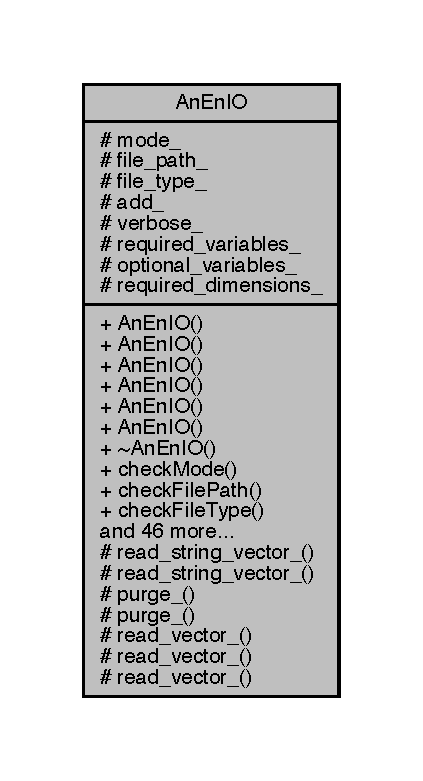
\includegraphics[width=203pt]{class_an_en_i_o__coll__graph}
\end{center}
\end{figure}
\subsection*{Public Types}
\begin{DoxyCompactItemize}
\item 
enum \mbox{\hyperlink{class_an_en_i_o_aa56bc1ec6610b86db4349bce20f9ead0}{error\+Type}} \{ \newline
\mbox{\hyperlink{class_an_en_i_o_aa56bc1ec6610b86db4349bce20f9ead0afd4f6d99fa57b8fd2d3f2298b1781f6d}{S\+U\+C\+C\+E\+SS}} = 0, 
\mbox{\hyperlink{class_an_en_i_o_aa56bc1ec6610b86db4349bce20f9ead0a307923ca3c0962a4fe341eb2d7eb1eaa}{U\+N\+K\+N\+O\+W\+N\+\_\+\+E\+R\+R\+OR}} = -\/1, 
\mbox{\hyperlink{class_an_en_i_o_aa56bc1ec6610b86db4349bce20f9ead0af27777283529d32c426e957fd4eba291}{U\+N\+K\+O\+W\+N\+\_\+\+F\+I\+L\+E\+\_\+\+T\+Y\+PE}} = -\/2, 
\mbox{\hyperlink{class_an_en_i_o_aa56bc1ec6610b86db4349bce20f9ead0a12593564dc1e16d72a57ba6016b1324f}{F\+I\+L\+E\+\_\+\+N\+O\+T\+\_\+\+F\+O\+U\+ND}} = -\/10, 
\newline
\mbox{\hyperlink{class_an_en_i_o_aa56bc1ec6610b86db4349bce20f9ead0a77597f2d2fa33ef922bd74ea4580d8b4}{R\+E\+Q\+U\+I\+R\+E\+D\+\_\+\+V\+A\+R\+I\+A\+B\+L\+E\+\_\+\+M\+I\+S\+S\+I\+NG}} = -\/11, 
\mbox{\hyperlink{class_an_en_i_o_aa56bc1ec6610b86db4349bce20f9ead0a0523be11226bd2aa810f5a30c124ab19}{O\+P\+T\+I\+O\+N\+A\+L\+\_\+\+V\+A\+R\+I\+A\+B\+L\+E\+\_\+\+M\+I\+S\+S\+I\+NG}} = -\/12, 
\mbox{\hyperlink{class_an_en_i_o_aa56bc1ec6610b86db4349bce20f9ead0ae1f7e1357e3be9b3312477eba02c07e0}{D\+I\+M\+E\+N\+S\+I\+O\+N\+\_\+\+M\+I\+S\+S\+I\+NG}} = -\/13, 
\mbox{\hyperlink{class_an_en_i_o_aa56bc1ec6610b86db4349bce20f9ead0a83d4d08faaa4e794e6b7fbb9a89f203e}{W\+R\+O\+N\+G\+\_\+\+V\+A\+R\+I\+A\+B\+L\+E\+\_\+\+S\+H\+A\+PE}} = -\/14, 
\newline
\mbox{\hyperlink{class_an_en_i_o_aa56bc1ec6610b86db4349bce20f9ead0ad8e12998f526437cb6b2450f16f46d51}{W\+R\+O\+N\+G\+\_\+\+V\+A\+R\+I\+A\+B\+L\+E\+\_\+\+T\+Y\+PE}} = -\/15, 
\mbox{\hyperlink{class_an_en_i_o_aa56bc1ec6610b86db4349bce20f9ead0a288f494fc6e909e8ee0b8a7f9c7ef9ca}{E\+L\+E\+M\+E\+N\+T\+\_\+\+N\+O\+T\+\_\+\+U\+N\+I\+Q\+UE}} = -\/16, 
\mbox{\hyperlink{class_an_en_i_o_aa56bc1ec6610b86db4349bce20f9ead0af58b3b49fb1d75cbafd2d8859e4c3a55}{E\+R\+R\+O\+R\+\_\+\+S\+E\+T\+T\+I\+N\+G\+\_\+\+V\+A\+L\+U\+ES}} = -\/50, 
\mbox{\hyperlink{class_an_en_i_o_aa56bc1ec6610b86db4349bce20f9ead0a0d5615cd010b41d905091ddea91f74b7}{I\+N\+S\+U\+F\+F\+I\+C\+I\+E\+N\+T\+\_\+\+M\+E\+M\+O\+RY}} = -\/100
 \}
\end{DoxyCompactItemize}
\subsection*{Public Member Functions}
\begin{DoxyCompactItemize}
\item 
\mbox{\hyperlink{class_an_en_i_o_a199f4cd2569599820126ae27ec25a647}{An\+En\+IO}} ()=delete
\item 
\mbox{\hyperlink{class_an_en_i_o_ab3dc8be2a5d7034cccd35ed72ee41275}{An\+En\+IO}} (const \mbox{\hyperlink{class_an_en_i_o}{An\+En\+IO}} \&orig)=delete
\item 
\mbox{\hyperlink{class_an_en_i_o_ad4b50b97a671e5063e08aa463e393a23}{An\+En\+IO}} (std\+::string file\+\_\+path)
\item 
\mbox{\hyperlink{class_an_en_i_o_af19d6df2100a5922affa88b37a825caf}{An\+En\+IO}} (std\+::string file\+\_\+path, std\+::string file\+\_\+type)
\item 
\mbox{\hyperlink{class_an_en_i_o_a6e33a9ad4a80aabf6c78aae3bcbbf8dd}{An\+En\+IO}} (std\+::string file\+\_\+path, std\+::string file\+\_\+type, int verbose)
\item 
\mbox{\hyperlink{class_an_en_i_o_a054dfff57b8d02d333020d9efb54f14a}{An\+En\+IO}} (std\+::string file\+\_\+path, std\+::string file\+\_\+type, int verbose, std\+::vector$<$ std\+::string $>$ required\+\_\+variables, std\+::vector$<$ std\+::string $>$ optional\+\_\+variables)
\item 
virtual \mbox{\hyperlink{class_an_en_i_o_a1e7aef95fd2a0c6aaef55998f48368f4}{$\sim$\+An\+En\+IO}} ()
\item 
\mbox{\hyperlink{class_an_en_i_o_aa56bc1ec6610b86db4349bce20f9ead0}{error\+Type}} \mbox{\hyperlink{class_an_en_i_o_adf0b96d441687159e1d884273847d68e}{check\+File}} () const
\item 
\mbox{\hyperlink{class_an_en_i_o_aa56bc1ec6610b86db4349bce20f9ead0}{error\+Type}} \mbox{\hyperlink{class_an_en_i_o_aa9b4700db58d0ef09af429d5d31ff55f}{check\+File\+Type}} () const
\item 
\mbox{\hyperlink{class_an_en_i_o_aa56bc1ec6610b86db4349bce20f9ead0}{error\+Type}} \mbox{\hyperlink{class_an_en_i_o_ab7f3ba245b7acb11184e0a5b3490a84b}{check\+Variable}} (std\+::string var\+\_\+name, bool optional) const
\item 
\mbox{\hyperlink{class_an_en_i_o_aa56bc1ec6610b86db4349bce20f9ead0}{error\+Type}} \mbox{\hyperlink{class_an_en_i_o_ab99f9aebd7b145de00fe15b8d4869ac2}{check\+Dim}} (string dim\+\_\+name) const
\item 
\mbox{\hyperlink{class_an_en_i_o_aa56bc1ec6610b86db4349bce20f9ead0}{error\+Type}} \mbox{\hyperlink{class_an_en_i_o_a44347f497bdf775fcf214ec75d8b6470}{check\+Variables}} () const
\item 
\mbox{\hyperlink{class_an_en_i_o_aa56bc1ec6610b86db4349bce20f9ead0}{error\+Type}} \mbox{\hyperlink{class_an_en_i_o_ab6cd06f6402655924002fec4f83195eb}{check\+Dimensions}} () const
\item 
\mbox{\hyperlink{class_an_en_i_o_aa56bc1ec6610b86db4349bce20f9ead0}{error\+Type}} \mbox{\hyperlink{class_an_en_i_o_a84b3e8dcfd3176b4ba20c5ff1b17ee85}{read\+Data}} (\mbox{\hyperlink{class_observations}{Observations}} \&observations)
\item 
\mbox{\hyperlink{class_an_en_i_o_aa56bc1ec6610b86db4349bce20f9ead0}{error\+Type}} \mbox{\hyperlink{class_an_en_i_o_aa00d954aadc03593981748c572010ffd}{read\+Data}} (\mbox{\hyperlink{class_forecasts}{Forecasts}} \&forecasts)
\item 
\mbox{\hyperlink{class_an_en_i_o_aa56bc1ec6610b86db4349bce20f9ead0}{error\+Type}} \mbox{\hyperlink{class_an_en_i_o_a7fdb924e4990c113e2e897310f9ce57c}{read\+F\+L\+Ts}} (\mbox{\hyperlink{class_f_l_ts}{F\+L\+Ts}} \&flts)
\item 
\mbox{\hyperlink{class_an_en_i_o_aa56bc1ec6610b86db4349bce20f9ead0}{error\+Type}} \mbox{\hyperlink{class_an_en_i_o_a909adad6126ab91d304d8bcc46bd5783}{read\+Parameters}} (\mbox{\hyperlink{class_parameters}{Parameters}} \&parameters)
\item 
\mbox{\hyperlink{class_an_en_i_o_aa56bc1ec6610b86db4349bce20f9ead0}{error\+Type}} \mbox{\hyperlink{class_an_en_i_o_a39c40b1ffcd5b12fc8991a0c47346f00}{read\+Stations}} (\mbox{\hyperlink{class_stations}{Stations}} \&stations)
\item 
\mbox{\hyperlink{class_an_en_i_o_aa56bc1ec6610b86db4349bce20f9ead0}{error\+Type}} \mbox{\hyperlink{class_an_en_i_o_a5c513a7a23000ea12419dc7687285612}{read\+Times}} (\mbox{\hyperlink{class_times}{Times}} \&times)
\item 
\mbox{\hyperlink{class_an_en_i_o_aa56bc1ec6610b86db4349bce20f9ead0}{error\+Type}} \mbox{\hyperlink{class_an_en_i_o_a5ca1c7df3da9720967d7ed06f2dfe09b}{read\+Dim\+Length}} (std\+::string dim\+\_\+name, std\+::size\+\_\+t \&len)
\item 
void \mbox{\hyperlink{class_an_en_i_o_a92276aeba9c0b5bd1cd3d285271d505f}{handle\+Error}} (const \mbox{\hyperlink{class_an_en_i_o_aa56bc1ec6610b86db4349bce20f9ead0}{error\+Type}} \&indicator) const
\item 
std\+::string \mbox{\hyperlink{class_an_en_i_o_aae00624f6127c7946496443f5322ec8e}{get\+File\+Path}} () const
\item 
std\+::string \mbox{\hyperlink{class_an_en_i_o_a6f51b190d64895a4ad907abcf4a10b75}{get\+File\+Type}} () const
\item 
std\+::vector$<$ std\+::string $>$ \mbox{\hyperlink{class_an_en_i_o_a50997e1baef5b8bb18d833c8c875a7bc}{get\+Optional\+Variables}} () const
\item 
std\+::vector$<$ std\+::string $>$ \mbox{\hyperlink{class_an_en_i_o_abd3cbf0e384dd9d610f985fb4131df9b}{get\+Required\+Variables}} () const
\item 
std\+::vector$<$ std\+::string $>$ \mbox{\hyperlink{class_an_en_i_o_ace777827f2548b3f06ce13f3ce4f4b6b}{get\+Required\+Dimensions}} () const
\item 
int \mbox{\hyperlink{class_an_en_i_o_a0bf0dab5e393c5597f97ab38c910e24d}{get\+Verbose}} () const
\item 
void \mbox{\hyperlink{class_an_en_i_o_a38bdc2d686737eba3812b3b41e073006}{set\+File\+Path}} (std\+::string \mbox{\hyperlink{class_an_en_i_o_ab892e06ca18be5e0c442c9e882e4475f}{file\+\_\+path\+\_\+}})
\item 
void \mbox{\hyperlink{class_an_en_i_o_ac1a951fd63d9b109e4574143e077f9b2}{set\+File\+Type}} (std\+::string file\+Type\+\_\+)
\item 
void \mbox{\hyperlink{class_an_en_i_o_abc499df15eac5fa3f203267723f5edfa}{set\+Optional\+Variables}} (std\+::vector$<$ std\+::string $>$ optional\+\_\+variables)
\item 
void \mbox{\hyperlink{class_an_en_i_o_a643c51c346118d8416fa2c2e0da8042a}{set\+Required\+Variables}} (std\+::vector$<$ std\+::string $>$ required\+\_\+variables)
\item 
void \mbox{\hyperlink{class_an_en_i_o_a239ea94b3648006920bcdcded4040ad3}{set\+Required\+Dimensions}} (std\+::vector$<$ std\+::string $>$ required\+\_\+dimensions)
\item 
void \mbox{\hyperlink{class_an_en_i_o_a696dff7bb250fc45b597e5f82e33e23e}{set\+Verbose}} (int \mbox{\hyperlink{class_an_en_i_o_a4f6abd007730e4a8f54d57cc3572bd9e}{verbose\+\_\+}})
\item 
void \mbox{\hyperlink{class_an_en_i_o_acd5682e81361d75ff5566ae1df5fa023}{dump\+Variable}} (std\+::string var\+\_\+name, std\+::size\+\_\+t start=0, std\+::size\+\_\+t count=0) const
\end{DoxyCompactItemize}
\subsection*{Protected Member Functions}
\begin{DoxyCompactItemize}
\item 
\mbox{\hyperlink{class_an_en_i_o_aa56bc1ec6610b86db4349bce20f9ead0}{error\+Type}} \mbox{\hyperlink{class_an_en_i_o_a17e7a4c520675c23b01cbd65c7ffe1d5}{read\+\_\+string\+\_\+vector\+\_\+}} (std\+::string var\+\_\+name, std\+::vector$<$ std\+::string $>$ \&vectors) const
\item 
{\footnotesize template$<$typename T $>$ }\\\mbox{\hyperlink{class_an_en_i_o_aa56bc1ec6610b86db4349bce20f9ead0}{error\+Type}} \mbox{\hyperlink{class_an_en_i_o_a3c3a3f86f90ea7610e086d371414d54f}{read\+\_\+vector\+\_\+}} (std\+::string var\+\_\+name, std\+::vector$<$ T $>$ \&vector) const
\end{DoxyCompactItemize}
\subsection*{Protected Attributes}
\begin{DoxyCompactItemize}
\item 
std\+::string \mbox{\hyperlink{class_an_en_i_o_ab892e06ca18be5e0c442c9e882e4475f}{file\+\_\+path\+\_\+}}
\item 
std\+::string \mbox{\hyperlink{class_an_en_i_o_addbfb455f641a394c14907163874d8fe}{file\+\_\+type\+\_\+}}
\item 
int \mbox{\hyperlink{class_an_en_i_o_a4f6abd007730e4a8f54d57cc3572bd9e}{verbose\+\_\+}} = 2
\item 
std\+::vector$<$ std\+::string $>$ \mbox{\hyperlink{class_an_en_i_o_a119dcb81d3811547f0e37d6c3752f0a7}{required\+\_\+variables\+\_\+}}
\item 
std\+::vector$<$ std\+::string $>$ \mbox{\hyperlink{class_an_en_i_o_a43f82ffbafbbda7ab8c9471d0bce70df}{optional\+\_\+variables\+\_\+}}
\item 
std\+::vector$<$ std\+::string $>$ \mbox{\hyperlink{class_an_en_i_o_adf42061631c78508bde00de7d22a65b4}{required\+\_\+dimensions\+\_\+}}
\end{DoxyCompactItemize}


\subsection{Member Enumeration Documentation}
\mbox{\Hypertarget{class_an_en_i_o_aa56bc1ec6610b86db4349bce20f9ead0}\label{class_an_en_i_o_aa56bc1ec6610b86db4349bce20f9ead0}} 
\index{An\+En\+IO@{An\+En\+IO}!error\+Type@{error\+Type}}
\index{error\+Type@{error\+Type}!An\+En\+IO@{An\+En\+IO}}
\subsubsection{\texorpdfstring{error\+Type}{errorType}}
{\footnotesize\ttfamily enum \mbox{\hyperlink{class_an_en_i_o_aa56bc1ec6610b86db4349bce20f9ead0}{An\+En\+I\+O\+::error\+Type}}}

Specifies the return error type of a function. Use \mbox{\hyperlink{class_an_en_i_o_a92276aeba9c0b5bd1cd3d285271d505f}{An\+En\+I\+O\+::handle\+Error}} to handle the returned error\+Type variable. \begin{DoxyEnumFields}{Enumerator}
\raisebox{\heightof{T}}[0pt][0pt]{\index{S\+U\+C\+C\+E\+SS@{S\+U\+C\+C\+E\+SS}!An\+En\+IO@{An\+En\+IO}}\index{An\+En\+IO@{An\+En\+IO}!S\+U\+C\+C\+E\+SS@{S\+U\+C\+C\+E\+SS}}}\mbox{\Hypertarget{class_an_en_i_o_aa56bc1ec6610b86db4349bce20f9ead0afd4f6d99fa57b8fd2d3f2298b1781f6d}\label{class_an_en_i_o_aa56bc1ec6610b86db4349bce20f9ead0afd4f6d99fa57b8fd2d3f2298b1781f6d}} 
S\+U\+C\+C\+E\+SS&\\
\hline

\raisebox{\heightof{T}}[0pt][0pt]{\index{U\+N\+K\+N\+O\+W\+N\+\_\+\+E\+R\+R\+OR@{U\+N\+K\+N\+O\+W\+N\+\_\+\+E\+R\+R\+OR}!An\+En\+IO@{An\+En\+IO}}\index{An\+En\+IO@{An\+En\+IO}!U\+N\+K\+N\+O\+W\+N\+\_\+\+E\+R\+R\+OR@{U\+N\+K\+N\+O\+W\+N\+\_\+\+E\+R\+R\+OR}}}\mbox{\Hypertarget{class_an_en_i_o_aa56bc1ec6610b86db4349bce20f9ead0a307923ca3c0962a4fe341eb2d7eb1eaa}\label{class_an_en_i_o_aa56bc1ec6610b86db4349bce20f9ead0a307923ca3c0962a4fe341eb2d7eb1eaa}} 
U\+N\+K\+N\+O\+W\+N\+\_\+\+E\+R\+R\+OR&\\
\hline

\raisebox{\heightof{T}}[0pt][0pt]{\index{U\+N\+K\+O\+W\+N\+\_\+\+F\+I\+L\+E\+\_\+\+T\+Y\+PE@{U\+N\+K\+O\+W\+N\+\_\+\+F\+I\+L\+E\+\_\+\+T\+Y\+PE}!An\+En\+IO@{An\+En\+IO}}\index{An\+En\+IO@{An\+En\+IO}!U\+N\+K\+O\+W\+N\+\_\+\+F\+I\+L\+E\+\_\+\+T\+Y\+PE@{U\+N\+K\+O\+W\+N\+\_\+\+F\+I\+L\+E\+\_\+\+T\+Y\+PE}}}\mbox{\Hypertarget{class_an_en_i_o_aa56bc1ec6610b86db4349bce20f9ead0af27777283529d32c426e957fd4eba291}\label{class_an_en_i_o_aa56bc1ec6610b86db4349bce20f9ead0af27777283529d32c426e957fd4eba291}} 
U\+N\+K\+O\+W\+N\+\_\+\+F\+I\+L\+E\+\_\+\+T\+Y\+PE&\\
\hline

\raisebox{\heightof{T}}[0pt][0pt]{\index{F\+I\+L\+E\+\_\+\+N\+O\+T\+\_\+\+F\+O\+U\+ND@{F\+I\+L\+E\+\_\+\+N\+O\+T\+\_\+\+F\+O\+U\+ND}!An\+En\+IO@{An\+En\+IO}}\index{An\+En\+IO@{An\+En\+IO}!F\+I\+L\+E\+\_\+\+N\+O\+T\+\_\+\+F\+O\+U\+ND@{F\+I\+L\+E\+\_\+\+N\+O\+T\+\_\+\+F\+O\+U\+ND}}}\mbox{\Hypertarget{class_an_en_i_o_aa56bc1ec6610b86db4349bce20f9ead0a12593564dc1e16d72a57ba6016b1324f}\label{class_an_en_i_o_aa56bc1ec6610b86db4349bce20f9ead0a12593564dc1e16d72a57ba6016b1324f}} 
F\+I\+L\+E\+\_\+\+N\+O\+T\+\_\+\+F\+O\+U\+ND&\\
\hline

\raisebox{\heightof{T}}[0pt][0pt]{\index{R\+E\+Q\+U\+I\+R\+E\+D\+\_\+\+V\+A\+R\+I\+A\+B\+L\+E\+\_\+\+M\+I\+S\+S\+I\+NG@{R\+E\+Q\+U\+I\+R\+E\+D\+\_\+\+V\+A\+R\+I\+A\+B\+L\+E\+\_\+\+M\+I\+S\+S\+I\+NG}!An\+En\+IO@{An\+En\+IO}}\index{An\+En\+IO@{An\+En\+IO}!R\+E\+Q\+U\+I\+R\+E\+D\+\_\+\+V\+A\+R\+I\+A\+B\+L\+E\+\_\+\+M\+I\+S\+S\+I\+NG@{R\+E\+Q\+U\+I\+R\+E\+D\+\_\+\+V\+A\+R\+I\+A\+B\+L\+E\+\_\+\+M\+I\+S\+S\+I\+NG}}}\mbox{\Hypertarget{class_an_en_i_o_aa56bc1ec6610b86db4349bce20f9ead0a77597f2d2fa33ef922bd74ea4580d8b4}\label{class_an_en_i_o_aa56bc1ec6610b86db4349bce20f9ead0a77597f2d2fa33ef922bd74ea4580d8b4}} 
R\+E\+Q\+U\+I\+R\+E\+D\+\_\+\+V\+A\+R\+I\+A\+B\+L\+E\+\_\+\+M\+I\+S\+S\+I\+NG&\\
\hline

\raisebox{\heightof{T}}[0pt][0pt]{\index{O\+P\+T\+I\+O\+N\+A\+L\+\_\+\+V\+A\+R\+I\+A\+B\+L\+E\+\_\+\+M\+I\+S\+S\+I\+NG@{O\+P\+T\+I\+O\+N\+A\+L\+\_\+\+V\+A\+R\+I\+A\+B\+L\+E\+\_\+\+M\+I\+S\+S\+I\+NG}!An\+En\+IO@{An\+En\+IO}}\index{An\+En\+IO@{An\+En\+IO}!O\+P\+T\+I\+O\+N\+A\+L\+\_\+\+V\+A\+R\+I\+A\+B\+L\+E\+\_\+\+M\+I\+S\+S\+I\+NG@{O\+P\+T\+I\+O\+N\+A\+L\+\_\+\+V\+A\+R\+I\+A\+B\+L\+E\+\_\+\+M\+I\+S\+S\+I\+NG}}}\mbox{\Hypertarget{class_an_en_i_o_aa56bc1ec6610b86db4349bce20f9ead0a0523be11226bd2aa810f5a30c124ab19}\label{class_an_en_i_o_aa56bc1ec6610b86db4349bce20f9ead0a0523be11226bd2aa810f5a30c124ab19}} 
O\+P\+T\+I\+O\+N\+A\+L\+\_\+\+V\+A\+R\+I\+A\+B\+L\+E\+\_\+\+M\+I\+S\+S\+I\+NG&\\
\hline

\raisebox{\heightof{T}}[0pt][0pt]{\index{D\+I\+M\+E\+N\+S\+I\+O\+N\+\_\+\+M\+I\+S\+S\+I\+NG@{D\+I\+M\+E\+N\+S\+I\+O\+N\+\_\+\+M\+I\+S\+S\+I\+NG}!An\+En\+IO@{An\+En\+IO}}\index{An\+En\+IO@{An\+En\+IO}!D\+I\+M\+E\+N\+S\+I\+O\+N\+\_\+\+M\+I\+S\+S\+I\+NG@{D\+I\+M\+E\+N\+S\+I\+O\+N\+\_\+\+M\+I\+S\+S\+I\+NG}}}\mbox{\Hypertarget{class_an_en_i_o_aa56bc1ec6610b86db4349bce20f9ead0ae1f7e1357e3be9b3312477eba02c07e0}\label{class_an_en_i_o_aa56bc1ec6610b86db4349bce20f9ead0ae1f7e1357e3be9b3312477eba02c07e0}} 
D\+I\+M\+E\+N\+S\+I\+O\+N\+\_\+\+M\+I\+S\+S\+I\+NG&\\
\hline

\raisebox{\heightof{T}}[0pt][0pt]{\index{W\+R\+O\+N\+G\+\_\+\+V\+A\+R\+I\+A\+B\+L\+E\+\_\+\+S\+H\+A\+PE@{W\+R\+O\+N\+G\+\_\+\+V\+A\+R\+I\+A\+B\+L\+E\+\_\+\+S\+H\+A\+PE}!An\+En\+IO@{An\+En\+IO}}\index{An\+En\+IO@{An\+En\+IO}!W\+R\+O\+N\+G\+\_\+\+V\+A\+R\+I\+A\+B\+L\+E\+\_\+\+S\+H\+A\+PE@{W\+R\+O\+N\+G\+\_\+\+V\+A\+R\+I\+A\+B\+L\+E\+\_\+\+S\+H\+A\+PE}}}\mbox{\Hypertarget{class_an_en_i_o_aa56bc1ec6610b86db4349bce20f9ead0a83d4d08faaa4e794e6b7fbb9a89f203e}\label{class_an_en_i_o_aa56bc1ec6610b86db4349bce20f9ead0a83d4d08faaa4e794e6b7fbb9a89f203e}} 
W\+R\+O\+N\+G\+\_\+\+V\+A\+R\+I\+A\+B\+L\+E\+\_\+\+S\+H\+A\+PE&\\
\hline

\raisebox{\heightof{T}}[0pt][0pt]{\index{W\+R\+O\+N\+G\+\_\+\+V\+A\+R\+I\+A\+B\+L\+E\+\_\+\+T\+Y\+PE@{W\+R\+O\+N\+G\+\_\+\+V\+A\+R\+I\+A\+B\+L\+E\+\_\+\+T\+Y\+PE}!An\+En\+IO@{An\+En\+IO}}\index{An\+En\+IO@{An\+En\+IO}!W\+R\+O\+N\+G\+\_\+\+V\+A\+R\+I\+A\+B\+L\+E\+\_\+\+T\+Y\+PE@{W\+R\+O\+N\+G\+\_\+\+V\+A\+R\+I\+A\+B\+L\+E\+\_\+\+T\+Y\+PE}}}\mbox{\Hypertarget{class_an_en_i_o_aa56bc1ec6610b86db4349bce20f9ead0ad8e12998f526437cb6b2450f16f46d51}\label{class_an_en_i_o_aa56bc1ec6610b86db4349bce20f9ead0ad8e12998f526437cb6b2450f16f46d51}} 
W\+R\+O\+N\+G\+\_\+\+V\+A\+R\+I\+A\+B\+L\+E\+\_\+\+T\+Y\+PE&\\
\hline

\raisebox{\heightof{T}}[0pt][0pt]{\index{E\+L\+E\+M\+E\+N\+T\+\_\+\+N\+O\+T\+\_\+\+U\+N\+I\+Q\+UE@{E\+L\+E\+M\+E\+N\+T\+\_\+\+N\+O\+T\+\_\+\+U\+N\+I\+Q\+UE}!An\+En\+IO@{An\+En\+IO}}\index{An\+En\+IO@{An\+En\+IO}!E\+L\+E\+M\+E\+N\+T\+\_\+\+N\+O\+T\+\_\+\+U\+N\+I\+Q\+UE@{E\+L\+E\+M\+E\+N\+T\+\_\+\+N\+O\+T\+\_\+\+U\+N\+I\+Q\+UE}}}\mbox{\Hypertarget{class_an_en_i_o_aa56bc1ec6610b86db4349bce20f9ead0a288f494fc6e909e8ee0b8a7f9c7ef9ca}\label{class_an_en_i_o_aa56bc1ec6610b86db4349bce20f9ead0a288f494fc6e909e8ee0b8a7f9c7ef9ca}} 
E\+L\+E\+M\+E\+N\+T\+\_\+\+N\+O\+T\+\_\+\+U\+N\+I\+Q\+UE&\\
\hline

\raisebox{\heightof{T}}[0pt][0pt]{\index{E\+R\+R\+O\+R\+\_\+\+S\+E\+T\+T\+I\+N\+G\+\_\+\+V\+A\+L\+U\+ES@{E\+R\+R\+O\+R\+\_\+\+S\+E\+T\+T\+I\+N\+G\+\_\+\+V\+A\+L\+U\+ES}!An\+En\+IO@{An\+En\+IO}}\index{An\+En\+IO@{An\+En\+IO}!E\+R\+R\+O\+R\+\_\+\+S\+E\+T\+T\+I\+N\+G\+\_\+\+V\+A\+L\+U\+ES@{E\+R\+R\+O\+R\+\_\+\+S\+E\+T\+T\+I\+N\+G\+\_\+\+V\+A\+L\+U\+ES}}}\mbox{\Hypertarget{class_an_en_i_o_aa56bc1ec6610b86db4349bce20f9ead0af58b3b49fb1d75cbafd2d8859e4c3a55}\label{class_an_en_i_o_aa56bc1ec6610b86db4349bce20f9ead0af58b3b49fb1d75cbafd2d8859e4c3a55}} 
E\+R\+R\+O\+R\+\_\+\+S\+E\+T\+T\+I\+N\+G\+\_\+\+V\+A\+L\+U\+ES&\\
\hline

\raisebox{\heightof{T}}[0pt][0pt]{\index{I\+N\+S\+U\+F\+F\+I\+C\+I\+E\+N\+T\+\_\+\+M\+E\+M\+O\+RY@{I\+N\+S\+U\+F\+F\+I\+C\+I\+E\+N\+T\+\_\+\+M\+E\+M\+O\+RY}!An\+En\+IO@{An\+En\+IO}}\index{An\+En\+IO@{An\+En\+IO}!I\+N\+S\+U\+F\+F\+I\+C\+I\+E\+N\+T\+\_\+\+M\+E\+M\+O\+RY@{I\+N\+S\+U\+F\+F\+I\+C\+I\+E\+N\+T\+\_\+\+M\+E\+M\+O\+RY}}}\mbox{\Hypertarget{class_an_en_i_o_aa56bc1ec6610b86db4349bce20f9ead0a0d5615cd010b41d905091ddea91f74b7}\label{class_an_en_i_o_aa56bc1ec6610b86db4349bce20f9ead0a0d5615cd010b41d905091ddea91f74b7}} 
I\+N\+S\+U\+F\+F\+I\+C\+I\+E\+N\+T\+\_\+\+M\+E\+M\+O\+RY&\\
\hline

\end{DoxyEnumFields}


\subsection{Constructor \& Destructor Documentation}
\mbox{\Hypertarget{class_an_en_i_o_a199f4cd2569599820126ae27ec25a647}\label{class_an_en_i_o_a199f4cd2569599820126ae27ec25a647}} 
\index{An\+En\+IO@{An\+En\+IO}!An\+En\+IO@{An\+En\+IO}}
\index{An\+En\+IO@{An\+En\+IO}!An\+En\+IO@{An\+En\+IO}}
\subsubsection{\texorpdfstring{An\+En\+I\+O()}{AnEnIO()}\hspace{0.1cm}{\footnotesize\ttfamily [1/6]}}
{\footnotesize\ttfamily An\+En\+I\+O\+::\+An\+En\+IO (\begin{DoxyParamCaption}{ }\end{DoxyParamCaption})\hspace{0.3cm}{\ttfamily [delete]}}

\mbox{\Hypertarget{class_an_en_i_o_ab3dc8be2a5d7034cccd35ed72ee41275}\label{class_an_en_i_o_ab3dc8be2a5d7034cccd35ed72ee41275}} 
\index{An\+En\+IO@{An\+En\+IO}!An\+En\+IO@{An\+En\+IO}}
\index{An\+En\+IO@{An\+En\+IO}!An\+En\+IO@{An\+En\+IO}}
\subsubsection{\texorpdfstring{An\+En\+I\+O()}{AnEnIO()}\hspace{0.1cm}{\footnotesize\ttfamily [2/6]}}
{\footnotesize\ttfamily An\+En\+I\+O\+::\+An\+En\+IO (\begin{DoxyParamCaption}\item[{const \mbox{\hyperlink{class_an_en_i_o}{An\+En\+IO}} \&}]{orig }\end{DoxyParamCaption})\hspace{0.3cm}{\ttfamily [delete]}}

\mbox{\Hypertarget{class_an_en_i_o_ad4b50b97a671e5063e08aa463e393a23}\label{class_an_en_i_o_ad4b50b97a671e5063e08aa463e393a23}} 
\index{An\+En\+IO@{An\+En\+IO}!An\+En\+IO@{An\+En\+IO}}
\index{An\+En\+IO@{An\+En\+IO}!An\+En\+IO@{An\+En\+IO}}
\subsubsection{\texorpdfstring{An\+En\+I\+O()}{AnEnIO()}\hspace{0.1cm}{\footnotesize\ttfamily [3/6]}}
{\footnotesize\ttfamily An\+En\+I\+O\+::\+An\+En\+IO (\begin{DoxyParamCaption}\item[{std\+::string}]{file\+\_\+path }\end{DoxyParamCaption})}

\mbox{\Hypertarget{class_an_en_i_o_af19d6df2100a5922affa88b37a825caf}\label{class_an_en_i_o_af19d6df2100a5922affa88b37a825caf}} 
\index{An\+En\+IO@{An\+En\+IO}!An\+En\+IO@{An\+En\+IO}}
\index{An\+En\+IO@{An\+En\+IO}!An\+En\+IO@{An\+En\+IO}}
\subsubsection{\texorpdfstring{An\+En\+I\+O()}{AnEnIO()}\hspace{0.1cm}{\footnotesize\ttfamily [4/6]}}
{\footnotesize\ttfamily An\+En\+I\+O\+::\+An\+En\+IO (\begin{DoxyParamCaption}\item[{std\+::string}]{file\+\_\+path,  }\item[{std\+::string}]{file\+\_\+type }\end{DoxyParamCaption})}

\mbox{\Hypertarget{class_an_en_i_o_a6e33a9ad4a80aabf6c78aae3bcbbf8dd}\label{class_an_en_i_o_a6e33a9ad4a80aabf6c78aae3bcbbf8dd}} 
\index{An\+En\+IO@{An\+En\+IO}!An\+En\+IO@{An\+En\+IO}}
\index{An\+En\+IO@{An\+En\+IO}!An\+En\+IO@{An\+En\+IO}}
\subsubsection{\texorpdfstring{An\+En\+I\+O()}{AnEnIO()}\hspace{0.1cm}{\footnotesize\ttfamily [5/6]}}
{\footnotesize\ttfamily An\+En\+I\+O\+::\+An\+En\+IO (\begin{DoxyParamCaption}\item[{std\+::string}]{file\+\_\+path,  }\item[{std\+::string}]{file\+\_\+type,  }\item[{int}]{verbose }\end{DoxyParamCaption})}

\mbox{\Hypertarget{class_an_en_i_o_a054dfff57b8d02d333020d9efb54f14a}\label{class_an_en_i_o_a054dfff57b8d02d333020d9efb54f14a}} 
\index{An\+En\+IO@{An\+En\+IO}!An\+En\+IO@{An\+En\+IO}}
\index{An\+En\+IO@{An\+En\+IO}!An\+En\+IO@{An\+En\+IO}}
\subsubsection{\texorpdfstring{An\+En\+I\+O()}{AnEnIO()}\hspace{0.1cm}{\footnotesize\ttfamily [6/6]}}
{\footnotesize\ttfamily An\+En\+I\+O\+::\+An\+En\+IO (\begin{DoxyParamCaption}\item[{std\+::string}]{file\+\_\+path,  }\item[{std\+::string}]{file\+\_\+type,  }\item[{int}]{verbose,  }\item[{std\+::vector$<$ std\+::string $>$}]{required\+\_\+variables,  }\item[{std\+::vector$<$ std\+::string $>$}]{optional\+\_\+variables }\end{DoxyParamCaption})}

\mbox{\Hypertarget{class_an_en_i_o_a1e7aef95fd2a0c6aaef55998f48368f4}\label{class_an_en_i_o_a1e7aef95fd2a0c6aaef55998f48368f4}} 
\index{An\+En\+IO@{An\+En\+IO}!````~An\+En\+IO@{$\sim$\+An\+En\+IO}}
\index{````~An\+En\+IO@{$\sim$\+An\+En\+IO}!An\+En\+IO@{An\+En\+IO}}
\subsubsection{\texorpdfstring{$\sim$\+An\+En\+I\+O()}{~AnEnIO()}}
{\footnotesize\ttfamily An\+En\+I\+O\+::$\sim$\+An\+En\+IO (\begin{DoxyParamCaption}{ }\end{DoxyParamCaption})\hspace{0.3cm}{\ttfamily [virtual]}}



\subsection{Member Function Documentation}
\mbox{\Hypertarget{class_an_en_i_o_ab99f9aebd7b145de00fe15b8d4869ac2}\label{class_an_en_i_o_ab99f9aebd7b145de00fe15b8d4869ac2}} 
\index{An\+En\+IO@{An\+En\+IO}!check\+Dim@{check\+Dim}}
\index{check\+Dim@{check\+Dim}!An\+En\+IO@{An\+En\+IO}}
\subsubsection{\texorpdfstring{check\+Dim()}{checkDim()}}
{\footnotesize\ttfamily \mbox{\hyperlink{class_an_en_i_o_aa56bc1ec6610b86db4349bce20f9ead0}{error\+Type}} An\+En\+I\+O\+::check\+Dim (\begin{DoxyParamCaption}\item[{string}]{dim\+\_\+name }\end{DoxyParamCaption}) const}

Checks whether the dimension exists.


\begin{DoxyParams}{Parameters}
{\em dim\+\_\+name} & The dimension name. \\
\hline
\end{DoxyParams}
\begin{DoxyReturn}{Returns}
\mbox{\hyperlink{class_an_en_i_o_aa56bc1ec6610b86db4349bce20f9ead0}{An\+En\+I\+O\+::error\+Type}}. 
\end{DoxyReturn}
\mbox{\Hypertarget{class_an_en_i_o_ab6cd06f6402655924002fec4f83195eb}\label{class_an_en_i_o_ab6cd06f6402655924002fec4f83195eb}} 
\index{An\+En\+IO@{An\+En\+IO}!check\+Dimensions@{check\+Dimensions}}
\index{check\+Dimensions@{check\+Dimensions}!An\+En\+IO@{An\+En\+IO}}
\subsubsection{\texorpdfstring{check\+Dimensions()}{checkDimensions()}}
{\footnotesize\ttfamily \mbox{\hyperlink{class_an_en_i_o_aa56bc1ec6610b86db4349bce20f9ead0}{error\+Type}} An\+En\+I\+O\+::check\+Dimensions (\begin{DoxyParamCaption}{ }\end{DoxyParamCaption}) const}

Checks the required dimensions. \begin{DoxyReturn}{Returns}
\mbox{\hyperlink{class_an_en_i_o_aa56bc1ec6610b86db4349bce20f9ead0}{An\+En\+I\+O\+::error\+Type}}. 
\end{DoxyReturn}
\mbox{\Hypertarget{class_an_en_i_o_adf0b96d441687159e1d884273847d68e}\label{class_an_en_i_o_adf0b96d441687159e1d884273847d68e}} 
\index{An\+En\+IO@{An\+En\+IO}!check\+File@{check\+File}}
\index{check\+File@{check\+File}!An\+En\+IO@{An\+En\+IO}}
\subsubsection{\texorpdfstring{check\+File()}{checkFile()}}
{\footnotesize\ttfamily \mbox{\hyperlink{class_an_en_i_o_aa56bc1ec6610b86db4349bce20f9ead0}{error\+Type}} An\+En\+I\+O\+::check\+File (\begin{DoxyParamCaption}{ }\end{DoxyParamCaption}) const}

Checks whether the Net\+C\+DF file exists.

\begin{DoxyReturn}{Returns}
\mbox{\hyperlink{class_an_en_i_o_aa56bc1ec6610b86db4349bce20f9ead0}{An\+En\+I\+O\+::error\+Type}}. 
\end{DoxyReturn}
\mbox{\Hypertarget{class_an_en_i_o_aa9b4700db58d0ef09af429d5d31ff55f}\label{class_an_en_i_o_aa9b4700db58d0ef09af429d5d31ff55f}} 
\index{An\+En\+IO@{An\+En\+IO}!check\+File\+Type@{check\+File\+Type}}
\index{check\+File\+Type@{check\+File\+Type}!An\+En\+IO@{An\+En\+IO}}
\subsubsection{\texorpdfstring{check\+File\+Type()}{checkFileType()}}
{\footnotesize\ttfamily \mbox{\hyperlink{class_an_en_i_o_aa56bc1ec6610b86db4349bce20f9ead0}{error\+Type}} An\+En\+I\+O\+::check\+File\+Type (\begin{DoxyParamCaption}{ }\end{DoxyParamCaption}) const}

Checks whether the Net\+C\+DF file conforms with the file type.

\begin{DoxyReturn}{Returns}
\mbox{\hyperlink{class_an_en_i_o_aa56bc1ec6610b86db4349bce20f9ead0}{An\+En\+I\+O\+::error\+Type}}. 
\end{DoxyReturn}
\mbox{\Hypertarget{class_an_en_i_o_ab7f3ba245b7acb11184e0a5b3490a84b}\label{class_an_en_i_o_ab7f3ba245b7acb11184e0a5b3490a84b}} 
\index{An\+En\+IO@{An\+En\+IO}!check\+Variable@{check\+Variable}}
\index{check\+Variable@{check\+Variable}!An\+En\+IO@{An\+En\+IO}}
\subsubsection{\texorpdfstring{check\+Variable()}{checkVariable()}}
{\footnotesize\ttfamily \mbox{\hyperlink{class_an_en_i_o_aa56bc1ec6610b86db4349bce20f9ead0}{error\+Type}} An\+En\+I\+O\+::check\+Variable (\begin{DoxyParamCaption}\item[{std\+::string}]{var\+\_\+name,  }\item[{bool}]{optional }\end{DoxyParamCaption}) const}

Checks whether the variable exists. 
\begin{DoxyParams}{Parameters}
{\em var\+\_\+name} & The variable name. \\
\hline
{\em optional} & Whether the variable is optional. \\
\hline
\end{DoxyParams}
\begin{DoxyReturn}{Returns}
\mbox{\hyperlink{class_an_en_i_o_aa56bc1ec6610b86db4349bce20f9ead0}{An\+En\+I\+O\+::error\+Type}}. 
\end{DoxyReturn}
\mbox{\Hypertarget{class_an_en_i_o_a44347f497bdf775fcf214ec75d8b6470}\label{class_an_en_i_o_a44347f497bdf775fcf214ec75d8b6470}} 
\index{An\+En\+IO@{An\+En\+IO}!check\+Variables@{check\+Variables}}
\index{check\+Variables@{check\+Variables}!An\+En\+IO@{An\+En\+IO}}
\subsubsection{\texorpdfstring{check\+Variables()}{checkVariables()}}
{\footnotesize\ttfamily \mbox{\hyperlink{class_an_en_i_o_aa56bc1ec6610b86db4349bce20f9ead0}{error\+Type}} An\+En\+I\+O\+::check\+Variables (\begin{DoxyParamCaption}{ }\end{DoxyParamCaption}) const}

Checks the required and optional variables. \begin{DoxyReturn}{Returns}
\mbox{\hyperlink{class_an_en_i_o_aa56bc1ec6610b86db4349bce20f9ead0}{An\+En\+I\+O\+::error\+Type}}. 
\end{DoxyReturn}
\mbox{\Hypertarget{class_an_en_i_o_acd5682e81361d75ff5566ae1df5fa023}\label{class_an_en_i_o_acd5682e81361d75ff5566ae1df5fa023}} 
\index{An\+En\+IO@{An\+En\+IO}!dump\+Variable@{dump\+Variable}}
\index{dump\+Variable@{dump\+Variable}!An\+En\+IO@{An\+En\+IO}}
\subsubsection{\texorpdfstring{dump\+Variable()}{dumpVariable()}}
{\footnotesize\ttfamily void An\+En\+I\+O\+::dump\+Variable (\begin{DoxyParamCaption}\item[{std\+::string}]{var\+\_\+name,  }\item[{std\+::size\+\_\+t}]{start = {\ttfamily 0},  }\item[{std\+::size\+\_\+t}]{count = {\ttfamily 0} }\end{DoxyParamCaption}) const}

\mbox{\Hypertarget{class_an_en_i_o_aae00624f6127c7946496443f5322ec8e}\label{class_an_en_i_o_aae00624f6127c7946496443f5322ec8e}} 
\index{An\+En\+IO@{An\+En\+IO}!get\+File\+Path@{get\+File\+Path}}
\index{get\+File\+Path@{get\+File\+Path}!An\+En\+IO@{An\+En\+IO}}
\subsubsection{\texorpdfstring{get\+File\+Path()}{getFilePath()}}
{\footnotesize\ttfamily string An\+En\+I\+O\+::get\+File\+Path (\begin{DoxyParamCaption}{ }\end{DoxyParamCaption}) const}

\mbox{\Hypertarget{class_an_en_i_o_a6f51b190d64895a4ad907abcf4a10b75}\label{class_an_en_i_o_a6f51b190d64895a4ad907abcf4a10b75}} 
\index{An\+En\+IO@{An\+En\+IO}!get\+File\+Type@{get\+File\+Type}}
\index{get\+File\+Type@{get\+File\+Type}!An\+En\+IO@{An\+En\+IO}}
\subsubsection{\texorpdfstring{get\+File\+Type()}{getFileType()}}
{\footnotesize\ttfamily string An\+En\+I\+O\+::get\+File\+Type (\begin{DoxyParamCaption}{ }\end{DoxyParamCaption}) const}

\mbox{\Hypertarget{class_an_en_i_o_a50997e1baef5b8bb18d833c8c875a7bc}\label{class_an_en_i_o_a50997e1baef5b8bb18d833c8c875a7bc}} 
\index{An\+En\+IO@{An\+En\+IO}!get\+Optional\+Variables@{get\+Optional\+Variables}}
\index{get\+Optional\+Variables@{get\+Optional\+Variables}!An\+En\+IO@{An\+En\+IO}}
\subsubsection{\texorpdfstring{get\+Optional\+Variables()}{getOptionalVariables()}}
{\footnotesize\ttfamily vector$<$ string $>$ An\+En\+I\+O\+::get\+Optional\+Variables (\begin{DoxyParamCaption}{ }\end{DoxyParamCaption}) const}

\mbox{\Hypertarget{class_an_en_i_o_ace777827f2548b3f06ce13f3ce4f4b6b}\label{class_an_en_i_o_ace777827f2548b3f06ce13f3ce4f4b6b}} 
\index{An\+En\+IO@{An\+En\+IO}!get\+Required\+Dimensions@{get\+Required\+Dimensions}}
\index{get\+Required\+Dimensions@{get\+Required\+Dimensions}!An\+En\+IO@{An\+En\+IO}}
\subsubsection{\texorpdfstring{get\+Required\+Dimensions()}{getRequiredDimensions()}}
{\footnotesize\ttfamily vector$<$ std\+::string $>$ An\+En\+I\+O\+::get\+Required\+Dimensions (\begin{DoxyParamCaption}{ }\end{DoxyParamCaption}) const}

\mbox{\Hypertarget{class_an_en_i_o_abd3cbf0e384dd9d610f985fb4131df9b}\label{class_an_en_i_o_abd3cbf0e384dd9d610f985fb4131df9b}} 
\index{An\+En\+IO@{An\+En\+IO}!get\+Required\+Variables@{get\+Required\+Variables}}
\index{get\+Required\+Variables@{get\+Required\+Variables}!An\+En\+IO@{An\+En\+IO}}
\subsubsection{\texorpdfstring{get\+Required\+Variables()}{getRequiredVariables()}}
{\footnotesize\ttfamily vector$<$ string $>$ An\+En\+I\+O\+::get\+Required\+Variables (\begin{DoxyParamCaption}{ }\end{DoxyParamCaption}) const}

\mbox{\Hypertarget{class_an_en_i_o_a0bf0dab5e393c5597f97ab38c910e24d}\label{class_an_en_i_o_a0bf0dab5e393c5597f97ab38c910e24d}} 
\index{An\+En\+IO@{An\+En\+IO}!get\+Verbose@{get\+Verbose}}
\index{get\+Verbose@{get\+Verbose}!An\+En\+IO@{An\+En\+IO}}
\subsubsection{\texorpdfstring{get\+Verbose()}{getVerbose()}}
{\footnotesize\ttfamily int An\+En\+I\+O\+::get\+Verbose (\begin{DoxyParamCaption}{ }\end{DoxyParamCaption}) const}

\mbox{\Hypertarget{class_an_en_i_o_a92276aeba9c0b5bd1cd3d285271d505f}\label{class_an_en_i_o_a92276aeba9c0b5bd1cd3d285271d505f}} 
\index{An\+En\+IO@{An\+En\+IO}!handle\+Error@{handle\+Error}}
\index{handle\+Error@{handle\+Error}!An\+En\+IO@{An\+En\+IO}}
\subsubsection{\texorpdfstring{handle\+Error()}{handleError()}}
{\footnotesize\ttfamily void An\+En\+I\+O\+::handle\+Error (\begin{DoxyParamCaption}\item[{const \mbox{\hyperlink{class_an_en_i_o_aa56bc1ec6610b86db4349bce20f9ead0}{error\+Type}} \&}]{indicator }\end{DoxyParamCaption}) const}

Handles the error\+Type variable.


\begin{DoxyParams}{Parameters}
{\em indicator} & An error\+Type item. \\
\hline
\end{DoxyParams}
\mbox{\Hypertarget{class_an_en_i_o_a17e7a4c520675c23b01cbd65c7ffe1d5}\label{class_an_en_i_o_a17e7a4c520675c23b01cbd65c7ffe1d5}} 
\index{An\+En\+IO@{An\+En\+IO}!read\+\_\+string\+\_\+vector\+\_\+@{read\+\_\+string\+\_\+vector\+\_\+}}
\index{read\+\_\+string\+\_\+vector\+\_\+@{read\+\_\+string\+\_\+vector\+\_\+}!An\+En\+IO@{An\+En\+IO}}
\subsubsection{\texorpdfstring{read\+\_\+string\+\_\+vector\+\_\+()}{read\_string\_vector\_()}}
{\footnotesize\ttfamily \mbox{\hyperlink{class_an_en_i_o_aa56bc1ec6610b86db4349bce20f9ead0}{error\+Type}} An\+En\+I\+O\+::read\+\_\+string\+\_\+vector\+\_\+ (\begin{DoxyParamCaption}\item[{std\+::string}]{var\+\_\+name,  }\item[{std\+::vector$<$ std\+::string $>$ \&}]{vectors }\end{DoxyParamCaption}) const\hspace{0.3cm}{\ttfamily [protected]}}

Reads variables as a string vector. The variable should has two dimensions and be the type of nc\+\_\+\+C\+H\+AR.


\begin{DoxyParams}{Parameters}
{\em var\+\_\+name} & The variable name. \\
\hline
{\em vectors} & A string container. \\
\hline
\end{DoxyParams}
\begin{DoxyReturn}{Returns}
\mbox{\hyperlink{class_an_en_i_o_aa56bc1ec6610b86db4349bce20f9ead0}{An\+En\+I\+O\+::error\+Type}}. 
\end{DoxyReturn}
\mbox{\Hypertarget{class_an_en_i_o_a3c3a3f86f90ea7610e086d371414d54f}\label{class_an_en_i_o_a3c3a3f86f90ea7610e086d371414d54f}} 
\index{An\+En\+IO@{An\+En\+IO}!read\+\_\+vector\+\_\+@{read\+\_\+vector\+\_\+}}
\index{read\+\_\+vector\+\_\+@{read\+\_\+vector\+\_\+}!An\+En\+IO@{An\+En\+IO}}
\subsubsection{\texorpdfstring{read\+\_\+vector\+\_\+()}{read\_vector\_()}}
{\footnotesize\ttfamily template$<$typename T $>$ \\
\mbox{\hyperlink{class_an_en_i_o_aa56bc1ec6610b86db4349bce20f9ead0}{error\+Type}} An\+En\+I\+O\+::read\+\_\+vector\+\_\+ (\begin{DoxyParamCaption}\item[{std\+::string}]{var\+\_\+name,  }\item[{std\+::vector$<$ T $>$ \&}]{vector }\end{DoxyParamCaption}) const\hspace{0.3cm}{\ttfamily [inline]}, {\ttfamily [protected]}}

Reads variables as a atomic vector.


\begin{DoxyParams}{Parameters}
{\em var\+\_\+name} & The variable name. \\
\hline
{\em vector} & An atmoic container. \\
\hline
\end{DoxyParams}
\begin{DoxyReturn}{Returns}
\mbox{\hyperlink{class_an_en_i_o_aa56bc1ec6610b86db4349bce20f9ead0}{An\+En\+I\+O\+::error\+Type}}. 
\end{DoxyReturn}
\mbox{\Hypertarget{class_an_en_i_o_a84b3e8dcfd3176b4ba20c5ff1b17ee85}\label{class_an_en_i_o_a84b3e8dcfd3176b4ba20c5ff1b17ee85}} 
\index{An\+En\+IO@{An\+En\+IO}!read\+Data@{read\+Data}}
\index{read\+Data@{read\+Data}!An\+En\+IO@{An\+En\+IO}}
\subsubsection{\texorpdfstring{read\+Data()}{readData()}\hspace{0.1cm}{\footnotesize\ttfamily [1/2]}}
{\footnotesize\ttfamily \mbox{\hyperlink{class_an_en_i_o_aa56bc1ec6610b86db4349bce20f9ead0}{error\+Type}} An\+En\+I\+O\+::read\+Data (\begin{DoxyParamCaption}\item[{\mbox{\hyperlink{class_observations}{Observations}} \&}]{observations }\end{DoxyParamCaption})}

\mbox{\Hypertarget{class_an_en_i_o_aa00d954aadc03593981748c572010ffd}\label{class_an_en_i_o_aa00d954aadc03593981748c572010ffd}} 
\index{An\+En\+IO@{An\+En\+IO}!read\+Data@{read\+Data}}
\index{read\+Data@{read\+Data}!An\+En\+IO@{An\+En\+IO}}
\subsubsection{\texorpdfstring{read\+Data()}{readData()}\hspace{0.1cm}{\footnotesize\ttfamily [2/2]}}
{\footnotesize\ttfamily \mbox{\hyperlink{class_an_en_i_o_aa56bc1ec6610b86db4349bce20f9ead0}{error\+Type}} An\+En\+I\+O\+::read\+Data (\begin{DoxyParamCaption}\item[{\mbox{\hyperlink{class_forecasts}{Forecasts}} \&}]{forecasts }\end{DoxyParamCaption})}

\mbox{\Hypertarget{class_an_en_i_o_a5ca1c7df3da9720967d7ed06f2dfe09b}\label{class_an_en_i_o_a5ca1c7df3da9720967d7ed06f2dfe09b}} 
\index{An\+En\+IO@{An\+En\+IO}!read\+Dim\+Length@{read\+Dim\+Length}}
\index{read\+Dim\+Length@{read\+Dim\+Length}!An\+En\+IO@{An\+En\+IO}}
\subsubsection{\texorpdfstring{read\+Dim\+Length()}{readDimLength()}}
{\footnotesize\ttfamily \mbox{\hyperlink{class_an_en_i_o_aa56bc1ec6610b86db4349bce20f9ead0}{error\+Type}} An\+En\+I\+O\+::read\+Dim\+Length (\begin{DoxyParamCaption}\item[{std\+::string}]{dim\+\_\+name,  }\item[{std\+::size\+\_\+t \&}]{len }\end{DoxyParamCaption})}

\mbox{\Hypertarget{class_an_en_i_o_a7fdb924e4990c113e2e897310f9ce57c}\label{class_an_en_i_o_a7fdb924e4990c113e2e897310f9ce57c}} 
\index{An\+En\+IO@{An\+En\+IO}!read\+F\+L\+Ts@{read\+F\+L\+Ts}}
\index{read\+F\+L\+Ts@{read\+F\+L\+Ts}!An\+En\+IO@{An\+En\+IO}}
\subsubsection{\texorpdfstring{read\+F\+L\+Ts()}{readFLTs()}}
{\footnotesize\ttfamily \mbox{\hyperlink{class_an_en_i_o_aa56bc1ec6610b86db4349bce20f9ead0}{error\+Type}} An\+En\+I\+O\+::read\+F\+L\+Ts (\begin{DoxyParamCaption}\item[{\mbox{\hyperlink{class_f_l_ts}{F\+L\+Ts}} \&}]{flts }\end{DoxyParamCaption})}

\mbox{\Hypertarget{class_an_en_i_o_a909adad6126ab91d304d8bcc46bd5783}\label{class_an_en_i_o_a909adad6126ab91d304d8bcc46bd5783}} 
\index{An\+En\+IO@{An\+En\+IO}!read\+Parameters@{read\+Parameters}}
\index{read\+Parameters@{read\+Parameters}!An\+En\+IO@{An\+En\+IO}}
\subsubsection{\texorpdfstring{read\+Parameters()}{readParameters()}}
{\footnotesize\ttfamily \mbox{\hyperlink{class_an_en_i_o_aa56bc1ec6610b86db4349bce20f9ead0}{error\+Type}} An\+En\+I\+O\+::read\+Parameters (\begin{DoxyParamCaption}\item[{\mbox{\hyperlink{class_parameters}{Parameters}} \&}]{parameters }\end{DoxyParamCaption})}

\mbox{\Hypertarget{class_an_en_i_o_a39c40b1ffcd5b12fc8991a0c47346f00}\label{class_an_en_i_o_a39c40b1ffcd5b12fc8991a0c47346f00}} 
\index{An\+En\+IO@{An\+En\+IO}!read\+Stations@{read\+Stations}}
\index{read\+Stations@{read\+Stations}!An\+En\+IO@{An\+En\+IO}}
\subsubsection{\texorpdfstring{read\+Stations()}{readStations()}}
{\footnotesize\ttfamily \mbox{\hyperlink{class_an_en_i_o_aa56bc1ec6610b86db4349bce20f9ead0}{error\+Type}} An\+En\+I\+O\+::read\+Stations (\begin{DoxyParamCaption}\item[{\mbox{\hyperlink{class_stations}{Stations}} \&}]{stations }\end{DoxyParamCaption})}

\mbox{\Hypertarget{class_an_en_i_o_a5c513a7a23000ea12419dc7687285612}\label{class_an_en_i_o_a5c513a7a23000ea12419dc7687285612}} 
\index{An\+En\+IO@{An\+En\+IO}!read\+Times@{read\+Times}}
\index{read\+Times@{read\+Times}!An\+En\+IO@{An\+En\+IO}}
\subsubsection{\texorpdfstring{read\+Times()}{readTimes()}}
{\footnotesize\ttfamily \mbox{\hyperlink{class_an_en_i_o_aa56bc1ec6610b86db4349bce20f9ead0}{error\+Type}} An\+En\+I\+O\+::read\+Times (\begin{DoxyParamCaption}\item[{\mbox{\hyperlink{class_times}{Times}} \&}]{times }\end{DoxyParamCaption})}

\mbox{\Hypertarget{class_an_en_i_o_a38bdc2d686737eba3812b3b41e073006}\label{class_an_en_i_o_a38bdc2d686737eba3812b3b41e073006}} 
\index{An\+En\+IO@{An\+En\+IO}!set\+File\+Path@{set\+File\+Path}}
\index{set\+File\+Path@{set\+File\+Path}!An\+En\+IO@{An\+En\+IO}}
\subsubsection{\texorpdfstring{set\+File\+Path()}{setFilePath()}}
{\footnotesize\ttfamily void An\+En\+I\+O\+::set\+File\+Path (\begin{DoxyParamCaption}\item[{std\+::string}]{file\+\_\+path\+\_\+ }\end{DoxyParamCaption})}

\mbox{\Hypertarget{class_an_en_i_o_ac1a951fd63d9b109e4574143e077f9b2}\label{class_an_en_i_o_ac1a951fd63d9b109e4574143e077f9b2}} 
\index{An\+En\+IO@{An\+En\+IO}!set\+File\+Type@{set\+File\+Type}}
\index{set\+File\+Type@{set\+File\+Type}!An\+En\+IO@{An\+En\+IO}}
\subsubsection{\texorpdfstring{set\+File\+Type()}{setFileType()}}
{\footnotesize\ttfamily void An\+En\+I\+O\+::set\+File\+Type (\begin{DoxyParamCaption}\item[{std\+::string}]{file\+Type\+\_\+ }\end{DoxyParamCaption})}

\mbox{\Hypertarget{class_an_en_i_o_abc499df15eac5fa3f203267723f5edfa}\label{class_an_en_i_o_abc499df15eac5fa3f203267723f5edfa}} 
\index{An\+En\+IO@{An\+En\+IO}!set\+Optional\+Variables@{set\+Optional\+Variables}}
\index{set\+Optional\+Variables@{set\+Optional\+Variables}!An\+En\+IO@{An\+En\+IO}}
\subsubsection{\texorpdfstring{set\+Optional\+Variables()}{setOptionalVariables()}}
{\footnotesize\ttfamily void An\+En\+I\+O\+::set\+Optional\+Variables (\begin{DoxyParamCaption}\item[{std\+::vector$<$ std\+::string $>$}]{optional\+\_\+variables }\end{DoxyParamCaption})}

\mbox{\Hypertarget{class_an_en_i_o_a239ea94b3648006920bcdcded4040ad3}\label{class_an_en_i_o_a239ea94b3648006920bcdcded4040ad3}} 
\index{An\+En\+IO@{An\+En\+IO}!set\+Required\+Dimensions@{set\+Required\+Dimensions}}
\index{set\+Required\+Dimensions@{set\+Required\+Dimensions}!An\+En\+IO@{An\+En\+IO}}
\subsubsection{\texorpdfstring{set\+Required\+Dimensions()}{setRequiredDimensions()}}
{\footnotesize\ttfamily void An\+En\+I\+O\+::set\+Required\+Dimensions (\begin{DoxyParamCaption}\item[{std\+::vector$<$ std\+::string $>$}]{required\+\_\+dimensions }\end{DoxyParamCaption})}

\mbox{\Hypertarget{class_an_en_i_o_a643c51c346118d8416fa2c2e0da8042a}\label{class_an_en_i_o_a643c51c346118d8416fa2c2e0da8042a}} 
\index{An\+En\+IO@{An\+En\+IO}!set\+Required\+Variables@{set\+Required\+Variables}}
\index{set\+Required\+Variables@{set\+Required\+Variables}!An\+En\+IO@{An\+En\+IO}}
\subsubsection{\texorpdfstring{set\+Required\+Variables()}{setRequiredVariables()}}
{\footnotesize\ttfamily void An\+En\+I\+O\+::set\+Required\+Variables (\begin{DoxyParamCaption}\item[{std\+::vector$<$ std\+::string $>$}]{required\+\_\+variables }\end{DoxyParamCaption})}

\mbox{\Hypertarget{class_an_en_i_o_a696dff7bb250fc45b597e5f82e33e23e}\label{class_an_en_i_o_a696dff7bb250fc45b597e5f82e33e23e}} 
\index{An\+En\+IO@{An\+En\+IO}!set\+Verbose@{set\+Verbose}}
\index{set\+Verbose@{set\+Verbose}!An\+En\+IO@{An\+En\+IO}}
\subsubsection{\texorpdfstring{set\+Verbose()}{setVerbose()}}
{\footnotesize\ttfamily void An\+En\+I\+O\+::set\+Verbose (\begin{DoxyParamCaption}\item[{int}]{verbose\+\_\+ }\end{DoxyParamCaption})}



\subsection{Member Data Documentation}
\mbox{\Hypertarget{class_an_en_i_o_ab892e06ca18be5e0c442c9e882e4475f}\label{class_an_en_i_o_ab892e06ca18be5e0c442c9e882e4475f}} 
\index{An\+En\+IO@{An\+En\+IO}!file\+\_\+path\+\_\+@{file\+\_\+path\+\_\+}}
\index{file\+\_\+path\+\_\+@{file\+\_\+path\+\_\+}!An\+En\+IO@{An\+En\+IO}}
\subsubsection{\texorpdfstring{file\+\_\+path\+\_\+}{file\_path\_}}
{\footnotesize\ttfamily std\+::string An\+En\+I\+O\+::file\+\_\+path\+\_\+\hspace{0.3cm}{\ttfamily [protected]}}

Specifies the full path to the file. \mbox{\Hypertarget{class_an_en_i_o_addbfb455f641a394c14907163874d8fe}\label{class_an_en_i_o_addbfb455f641a394c14907163874d8fe}} 
\index{An\+En\+IO@{An\+En\+IO}!file\+\_\+type\+\_\+@{file\+\_\+type\+\_\+}}
\index{file\+\_\+type\+\_\+@{file\+\_\+type\+\_\+}!An\+En\+IO@{An\+En\+IO}}
\subsubsection{\texorpdfstring{file\+\_\+type\+\_\+}{file\_type\_}}
{\footnotesize\ttfamily std\+::string An\+En\+I\+O\+::file\+\_\+type\+\_\+\hspace{0.3cm}{\ttfamily [protected]}}

Specifies the type of the file. The Value comes from An\+En\+I\+O\+::file\+Type. \mbox{\Hypertarget{class_an_en_i_o_a43f82ffbafbbda7ab8c9471d0bce70df}\label{class_an_en_i_o_a43f82ffbafbbda7ab8c9471d0bce70df}} 
\index{An\+En\+IO@{An\+En\+IO}!optional\+\_\+variables\+\_\+@{optional\+\_\+variables\+\_\+}}
\index{optional\+\_\+variables\+\_\+@{optional\+\_\+variables\+\_\+}!An\+En\+IO@{An\+En\+IO}}
\subsubsection{\texorpdfstring{optional\+\_\+variables\+\_\+}{optional\_variables\_}}
{\footnotesize\ttfamily std\+::vector$<$std\+::string$>$ An\+En\+I\+O\+::optional\+\_\+variables\+\_\+\hspace{0.3cm}{\ttfamily [protected]}}

Specifies the optional variable names in the file. \mbox{\Hypertarget{class_an_en_i_o_adf42061631c78508bde00de7d22a65b4}\label{class_an_en_i_o_adf42061631c78508bde00de7d22a65b4}} 
\index{An\+En\+IO@{An\+En\+IO}!required\+\_\+dimensions\+\_\+@{required\+\_\+dimensions\+\_\+}}
\index{required\+\_\+dimensions\+\_\+@{required\+\_\+dimensions\+\_\+}!An\+En\+IO@{An\+En\+IO}}
\subsubsection{\texorpdfstring{required\+\_\+dimensions\+\_\+}{required\_dimensions\_}}
{\footnotesize\ttfamily std\+::vector$<$std\+::string$>$ An\+En\+I\+O\+::required\+\_\+dimensions\+\_\+\hspace{0.3cm}{\ttfamily [protected]}}

Specifies the required dimension names in the file. \mbox{\Hypertarget{class_an_en_i_o_a119dcb81d3811547f0e37d6c3752f0a7}\label{class_an_en_i_o_a119dcb81d3811547f0e37d6c3752f0a7}} 
\index{An\+En\+IO@{An\+En\+IO}!required\+\_\+variables\+\_\+@{required\+\_\+variables\+\_\+}}
\index{required\+\_\+variables\+\_\+@{required\+\_\+variables\+\_\+}!An\+En\+IO@{An\+En\+IO}}
\subsubsection{\texorpdfstring{required\+\_\+variables\+\_\+}{required\_variables\_}}
{\footnotesize\ttfamily std\+::vector$<$std\+::string$>$ An\+En\+I\+O\+::required\+\_\+variables\+\_\+\hspace{0.3cm}{\ttfamily [protected]}}

Specifies the required variable names in the file. \mbox{\Hypertarget{class_an_en_i_o_a4f6abd007730e4a8f54d57cc3572bd9e}\label{class_an_en_i_o_a4f6abd007730e4a8f54d57cc3572bd9e}} 
\index{An\+En\+IO@{An\+En\+IO}!verbose\+\_\+@{verbose\+\_\+}}
\index{verbose\+\_\+@{verbose\+\_\+}!An\+En\+IO@{An\+En\+IO}}
\subsubsection{\texorpdfstring{verbose\+\_\+}{verbose\_}}
{\footnotesize\ttfamily int An\+En\+I\+O\+::verbose\+\_\+ = 2\hspace{0.3cm}{\ttfamily [protected]}}

Specifies the verbose level.
\begin{DoxyItemize}
\item 0\+: No standard output.
\item 1\+: Errors.
\item 2\+: The above plus Warnings.
\item 3\+: The above plus program progress information.
\item 4\+: The above plus session information. 
\end{DoxyItemize}

The documentation for this class was generated from the following files\+:\begin{DoxyCompactItemize}
\item 
\mbox{\hyperlink{_an_en_i_o_8h}{An\+En\+I\+O.\+h}}\item 
\mbox{\hyperlink{_an_en_i_o_8cpp}{An\+En\+I\+O.\+cpp}}\end{DoxyCompactItemize}

\hypertarget{class_array4_d}{}\section{Array4D Class Reference}
\label{class_array4_d}\index{Array4D@{Array4D}}


{\ttfamily \#include $<$Array4\+D.\+h$>$}



Inheritance diagram for Array4D\+:\nopagebreak
\begin{figure}[H]
\begin{center}
\leavevmode
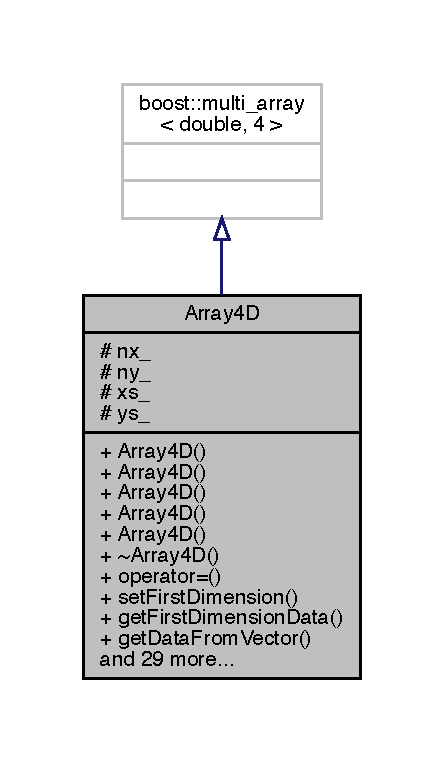
\includegraphics[width=213pt]{class_array4_d__inherit__graph}
\end{center}
\end{figure}


Collaboration diagram for Array4D\+:\nopagebreak
\begin{figure}[H]
\begin{center}
\leavevmode
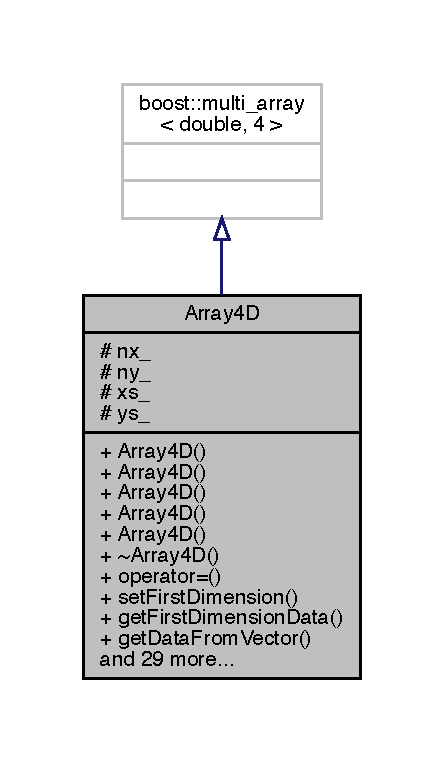
\includegraphics[width=213pt]{class_array4_d__coll__graph}
\end{center}
\end{figure}
\subsection*{Public Member Functions}
\begin{DoxyCompactItemize}
\item 
\mbox{\hyperlink{class_array4_d_a1bc84c0dcc22ed0e218040b01f56b816}{Array4D}} ()
\item 
\mbox{\hyperlink{class_array4_d_a7395b077e949df98c4cfe0c0aa93f2a8}{Array4D}} (const \mbox{\hyperlink{class_array4_d}{Array4D}} \&)
\item 
\mbox{\hyperlink{class_array4_d_a2b0e0536b5e40fec5694fdcaebdcff6a}{Array4D}} (size\+\_\+t d1, size\+\_\+t d2, size\+\_\+t d3, size\+\_\+t d4)
\item 
\mbox{\hyperlink{class_array4_d_a8ee78d0fd3a893d067386b1afd9a742e}{Array4D}} (std\+::vector$<$ double $>$ const \&, size\+\_\+t M, size\+\_\+t N, size\+\_\+t O, size\+\_\+t P)
\item 
\mbox{\hyperlink{class_array4_d_a5c5b3aa5f576edefc2e9a61afa87e451}{Array4D}} (Array4\+D\+::array\+\_\+view$<$ 4 $>$\+::type \&)
\item 
virtual \mbox{\hyperlink{class_array4_d_ae82ddfe43f803f16e7904dc839b63eab}{$\sim$\+Array4D}} ()
\item 
\mbox{\hyperlink{class_array4_d}{Array4D}} \& \mbox{\hyperlink{class_array4_d_aa56a432098cf289a2cc340dfc5635634}{operator=}} (const \mbox{\hyperlink{class_array4_d}{Array4D}} \&rhs)
\item 
void \mbox{\hyperlink{class_array4_d_a27a7b3dc2759941c5849a3843d9ad5d1}{set\+First\+Dimension}} (std\+::vector$<$ double $>$ const \&data, size\+\_\+t pos)
\item 
void \mbox{\hyperlink{class_array4_d_ac4d55dadfae71139e8d860fe171146c7}{get\+First\+Dimension\+Data}} (std\+::vector$<$ double $>$ \&data, size\+\_\+t pos)
\item 
void \mbox{\hyperlink{class_array4_d_af6879e11496cc7a736b813bbdeccd5d5}{set\+Data\+From\+Vector}} (std\+::vector$<$ double $>$ const \&data, size\+\_\+t M, size\+\_\+t N, size\+\_\+t O, size\+\_\+t P)
\item 
bool \mbox{\hyperlink{class_array4_d_abbcf6caa1305cd5709e6f194e961614d}{is\+Circular}} (size\+\_\+t pos) const
\item 
void \mbox{\hyperlink{class_array4_d_ab4574e45a22610a3e9768542afe76797}{set\+Circular}} (size\+\_\+t pos)
\item 
void \mbox{\hyperlink{class_array4_d_ac6d1282e0d765748c192a72d60274853}{unset\+Circular}} (size\+\_\+t pos)
\item 
bool \mbox{\hyperlink{class_array4_d_a8715e92d0a11f73a16ac3d67b7527f86}{set\+Names}} (const std\+::vector$<$ std\+::string $>$ \&new\+Names)
\item 
bool \mbox{\hyperlink{class_array4_d_a921401f1e3a471b6b5665d718c636daf}{set\+Name}} (size\+\_\+t pos, const std\+::string \&new\+Name)
\item 
std\+::string \mbox{\hyperlink{class_array4_d_a21932242976a122108f7cdf845f7aeca}{get\+Name}} (size\+\_\+t pos)
\item 
size\+\_\+t \mbox{\hyperlink{class_array4_d_afc2d361e388a5faba62caef697033911}{get\+Size\+Dim0}} () const
\item 
size\+\_\+t \mbox{\hyperlink{class_array4_d_a32f89196e8a5384f8a207812376f716d}{get\+Size\+Dim1}} () const
\item 
size\+\_\+t \mbox{\hyperlink{class_array4_d_abc321f73fd2665ac1c58afaf3ebe60e6}{get\+Size\+Dim2}} () const
\item 
size\+\_\+t \mbox{\hyperlink{class_array4_d_af767db0beba39cd815b903a8076d2695}{get\+Size\+Dim3}} () const
\item 
bool \mbox{\hyperlink{class_array4_d_ae829ad7badd47b721a9ecea2324f3168}{myresize}} (index, index, index, index)
\item 
void \mbox{\hyperlink{class_array4_d_a15626fe44d3792ccc2822afb30bcbd98}{randomize}} ()
\item 
void \mbox{\hyperlink{class_array4_d_ad4bf624213ab880802c14204a54bb1b4}{print}} (std\+::ostream \&) const
\item 
void \mbox{\hyperlink{class_array4_d_a838161eccbcb59c67d8ec5167e710cb2}{print\+\_\+size}} (std\+::ostream \&) const
\item 
size\+\_\+t \mbox{\hyperlink{class_array4_d_a2f9f3a7f699f705ebbc3067adf923922}{get\+\_\+nx}} ()
\item 
size\+\_\+t \mbox{\hyperlink{class_array4_d_a6f75a07d72213eff83aabbfd8442d1d3}{get\+\_\+ny}} ()
\item 
bool \mbox{\hyperlink{class_array4_d_a4071001d8fd5248bcaf89c54556a6fe2}{set\+\_\+nx\+\_\+ny}} (size\+\_\+t nx, size\+\_\+t ny)
\item 
const std\+::vector$<$ double $>$ \& \mbox{\hyperlink{class_array4_d_a5b72fa60e0feacd807d4d2e7bd1bf5fd}{get\+\_\+xs}} () const
\item 
const std\+::vector$<$ double $>$ \& \mbox{\hyperlink{class_array4_d_a3f6fa1fc8bc07a3aa51cbdada40e25e7}{get\+\_\+ys}} () const
\item 
bool \mbox{\hyperlink{class_array4_d_a66b2635ff1ce8ef57e9c55bba8e2bbda}{empty\+\_\+xs}} () const
\item 
bool \mbox{\hyperlink{class_array4_d_a40d87667978c6824f536367dcffbac39}{empty\+\_\+ys}} () const
\item 
size\+\_\+t \mbox{\hyperlink{class_array4_d_a440c545fcf694923767581f590d808df}{xs\+\_\+size}} () const
\item 
size\+\_\+t \mbox{\hyperlink{class_array4_d_a7c08ac86562c729d9fa24165cba55a97}{ys\+\_\+size}} () const
\item 
bool \mbox{\hyperlink{class_array4_d_a92afa660eb005779a0c2cf602aa4c6fe}{set\+\_\+xs}} (std\+::vector$<$ double $>$ input)
\item 
bool \mbox{\hyperlink{class_array4_d_a03ed88518d6991a55f3e48ad7de15d73}{set\+\_\+ys}} (std\+::vector$<$ double $>$ input)
\item 
double \mbox{\hyperlink{class_array4_d_a4668c9767181db6bd228e054a3f81696}{xs\+\_\+max}} () const
\item 
double \mbox{\hyperlink{class_array4_d_a642efdce56ea7ffaf7e24ed1d63b3151}{xs\+\_\+min}} () const
\item 
double \mbox{\hyperlink{class_array4_d_a1e142285afbb8b00662d8f77f0b92b80}{ys\+\_\+max}} () const
\item 
double \mbox{\hyperlink{class_array4_d_af27f181faf93d0ca96e65b1e5bdab82d}{ys\+\_\+min}} () const
\end{DoxyCompactItemize}
\subsection*{Protected Attributes}
\begin{DoxyCompactItemize}
\item 
size\+\_\+t \mbox{\hyperlink{class_array4_d_a5fa707d43fe236f8890dae010de99bf1}{nx\+\_\+}} = 0
\item 
size\+\_\+t \mbox{\hyperlink{class_array4_d_a0c3053b1362730bb52d2d6e9c4402099}{ny\+\_\+}} = 0
\item 
std\+::vector$<$ double $>$ \mbox{\hyperlink{class_array4_d_a6fdbbc14cbe18e25f68ec9773df18783}{xs\+\_\+}}
\item 
std\+::vector$<$ double $>$ \mbox{\hyperlink{class_array4_d_aa9277734c8de6f2a02e6b06ccccbdaad}{ys\+\_\+}}
\end{DoxyCompactItemize}
\subsection*{Friends}
\begin{DoxyCompactItemize}
\item 
std\+::ostream \& \mbox{\hyperlink{class_array4_d_af0c2770deee0bf3f3fc90fc3ea22147c}{operator$<$$<$}} (std\+::ostream \&, \mbox{\hyperlink{class_array4_d}{Array4D}} const \&)
\end{DoxyCompactItemize}


\subsection{Detailed Description}
GC\+: This is the basic data structure that is used to store the forecasts and the observations. Normally the data is stored in the following format\+:

\mbox{[}\mbox{\hyperlink{class_parameter}{Parameter}}\mbox{]}\mbox{[}\mbox{\hyperlink{class_station}{Station}}\mbox{]}\mbox{[}Days\mbox{]}\mbox{[}Forecast Lead Time\mbox{]}

It is assumed that all the data is stored as double. It has not been templated for optimization purposes, but it should be rather trivial to make this class work with different data types.

The class extends the functionality of the boost multidimensional array structure, which is used as the underlying container for the data. Although defining a built 4D array could lead to an increase in speed, it is not possible to use standard S\+TL paradigm and algorithms. The boost library allows for a transparent integration with S\+TL, and provides an optimized data structure bug free. The library is currently maintained and used worldwide. 

\subsection{Constructor \& Destructor Documentation}
\mbox{\Hypertarget{class_array4_d_a1bc84c0dcc22ed0e218040b01f56b816}\label{class_array4_d_a1bc84c0dcc22ed0e218040b01f56b816}} 
\index{Array4D@{Array4D}!Array4D@{Array4D}}
\index{Array4D@{Array4D}!Array4D@{Array4D}}
\subsubsection{\texorpdfstring{Array4\+D()}{Array4D()}\hspace{0.1cm}{\footnotesize\ttfamily [1/5]}}
{\footnotesize\ttfamily Array4\+D\+::\+Array4D (\begin{DoxyParamCaption}{ }\end{DoxyParamCaption})}

\mbox{\Hypertarget{class_array4_d_a7395b077e949df98c4cfe0c0aa93f2a8}\label{class_array4_d_a7395b077e949df98c4cfe0c0aa93f2a8}} 
\index{Array4D@{Array4D}!Array4D@{Array4D}}
\index{Array4D@{Array4D}!Array4D@{Array4D}}
\subsubsection{\texorpdfstring{Array4\+D()}{Array4D()}\hspace{0.1cm}{\footnotesize\ttfamily [2/5]}}
{\footnotesize\ttfamily Array4\+D\+::\+Array4D (\begin{DoxyParamCaption}\item[{const \mbox{\hyperlink{class_array4_d}{Array4D}} \&}]{rhs }\end{DoxyParamCaption})}

\mbox{\Hypertarget{class_array4_d_a2b0e0536b5e40fec5694fdcaebdcff6a}\label{class_array4_d_a2b0e0536b5e40fec5694fdcaebdcff6a}} 
\index{Array4D@{Array4D}!Array4D@{Array4D}}
\index{Array4D@{Array4D}!Array4D@{Array4D}}
\subsubsection{\texorpdfstring{Array4\+D()}{Array4D()}\hspace{0.1cm}{\footnotesize\ttfamily [3/5]}}
{\footnotesize\ttfamily Array4\+D\+::\+Array4D (\begin{DoxyParamCaption}\item[{size\+\_\+t}]{d1,  }\item[{size\+\_\+t}]{d2,  }\item[{size\+\_\+t}]{d3,  }\item[{size\+\_\+t}]{d4 }\end{DoxyParamCaption})}

\mbox{\Hypertarget{class_array4_d_a8ee78d0fd3a893d067386b1afd9a742e}\label{class_array4_d_a8ee78d0fd3a893d067386b1afd9a742e}} 
\index{Array4D@{Array4D}!Array4D@{Array4D}}
\index{Array4D@{Array4D}!Array4D@{Array4D}}
\subsubsection{\texorpdfstring{Array4\+D()}{Array4D()}\hspace{0.1cm}{\footnotesize\ttfamily [4/5]}}
{\footnotesize\ttfamily Array4\+D\+::\+Array4D (\begin{DoxyParamCaption}\item[{std\+::vector$<$ double $>$ const \&}]{,  }\item[{size\+\_\+t}]{M,  }\item[{size\+\_\+t}]{N,  }\item[{size\+\_\+t}]{O,  }\item[{size\+\_\+t}]{P }\end{DoxyParamCaption})}

\mbox{\Hypertarget{class_array4_d_a5c5b3aa5f576edefc2e9a61afa87e451}\label{class_array4_d_a5c5b3aa5f576edefc2e9a61afa87e451}} 
\index{Array4D@{Array4D}!Array4D@{Array4D}}
\index{Array4D@{Array4D}!Array4D@{Array4D}}
\subsubsection{\texorpdfstring{Array4\+D()}{Array4D()}\hspace{0.1cm}{\footnotesize\ttfamily [5/5]}}
{\footnotesize\ttfamily Array4\+D\+::\+Array4D (\begin{DoxyParamCaption}\item[{Array4\+D\+::array\+\_\+view$<$ 4 $>$\+::type \&}]{view }\end{DoxyParamCaption})}

\mbox{\Hypertarget{class_array4_d_ae82ddfe43f803f16e7904dc839b63eab}\label{class_array4_d_ae82ddfe43f803f16e7904dc839b63eab}} 
\index{Array4D@{Array4D}!````~Array4D@{$\sim$\+Array4D}}
\index{````~Array4D@{$\sim$\+Array4D}!Array4D@{Array4D}}
\subsubsection{\texorpdfstring{$\sim$\+Array4\+D()}{~Array4D()}}
{\footnotesize\ttfamily Array4\+D\+::$\sim$\+Array4D (\begin{DoxyParamCaption}{ }\end{DoxyParamCaption})\hspace{0.3cm}{\ttfamily [virtual]}}



\subsection{Member Function Documentation}
\mbox{\Hypertarget{class_array4_d_a66b2635ff1ce8ef57e9c55bba8e2bbda}\label{class_array4_d_a66b2635ff1ce8ef57e9c55bba8e2bbda}} 
\index{Array4D@{Array4D}!empty\+\_\+xs@{empty\+\_\+xs}}
\index{empty\+\_\+xs@{empty\+\_\+xs}!Array4D@{Array4D}}
\subsubsection{\texorpdfstring{empty\+\_\+xs()}{empty\_xs()}}
{\footnotesize\ttfamily bool Array4\+D\+::empty\+\_\+xs (\begin{DoxyParamCaption}{ }\end{DoxyParamCaption}) const}

\mbox{\Hypertarget{class_array4_d_a40d87667978c6824f536367dcffbac39}\label{class_array4_d_a40d87667978c6824f536367dcffbac39}} 
\index{Array4D@{Array4D}!empty\+\_\+ys@{empty\+\_\+ys}}
\index{empty\+\_\+ys@{empty\+\_\+ys}!Array4D@{Array4D}}
\subsubsection{\texorpdfstring{empty\+\_\+ys()}{empty\_ys()}}
{\footnotesize\ttfamily bool Array4\+D\+::empty\+\_\+ys (\begin{DoxyParamCaption}{ }\end{DoxyParamCaption}) const}

\mbox{\Hypertarget{class_array4_d_a2f9f3a7f699f705ebbc3067adf923922}\label{class_array4_d_a2f9f3a7f699f705ebbc3067adf923922}} 
\index{Array4D@{Array4D}!get\+\_\+nx@{get\+\_\+nx}}
\index{get\+\_\+nx@{get\+\_\+nx}!Array4D@{Array4D}}
\subsubsection{\texorpdfstring{get\+\_\+nx()}{get\_nx()}}
{\footnotesize\ttfamily size\+\_\+t Array4\+D\+::get\+\_\+nx (\begin{DoxyParamCaption}{ }\end{DoxyParamCaption})}

\mbox{\Hypertarget{class_array4_d_a6f75a07d72213eff83aabbfd8442d1d3}\label{class_array4_d_a6f75a07d72213eff83aabbfd8442d1d3}} 
\index{Array4D@{Array4D}!get\+\_\+ny@{get\+\_\+ny}}
\index{get\+\_\+ny@{get\+\_\+ny}!Array4D@{Array4D}}
\subsubsection{\texorpdfstring{get\+\_\+ny()}{get\_ny()}}
{\footnotesize\ttfamily size\+\_\+t Array4\+D\+::get\+\_\+ny (\begin{DoxyParamCaption}{ }\end{DoxyParamCaption})}

\mbox{\Hypertarget{class_array4_d_a5b72fa60e0feacd807d4d2e7bd1bf5fd}\label{class_array4_d_a5b72fa60e0feacd807d4d2e7bd1bf5fd}} 
\index{Array4D@{Array4D}!get\+\_\+xs@{get\+\_\+xs}}
\index{get\+\_\+xs@{get\+\_\+xs}!Array4D@{Array4D}}
\subsubsection{\texorpdfstring{get\+\_\+xs()}{get\_xs()}}
{\footnotesize\ttfamily const vector$<$ double $>$ \& Array4\+D\+::get\+\_\+xs (\begin{DoxyParamCaption}{ }\end{DoxyParamCaption}) const}

\mbox{\Hypertarget{class_array4_d_a3f6fa1fc8bc07a3aa51cbdada40e25e7}\label{class_array4_d_a3f6fa1fc8bc07a3aa51cbdada40e25e7}} 
\index{Array4D@{Array4D}!get\+\_\+ys@{get\+\_\+ys}}
\index{get\+\_\+ys@{get\+\_\+ys}!Array4D@{Array4D}}
\subsubsection{\texorpdfstring{get\+\_\+ys()}{get\_ys()}}
{\footnotesize\ttfamily const vector$<$ double $>$ \& Array4\+D\+::get\+\_\+ys (\begin{DoxyParamCaption}{ }\end{DoxyParamCaption}) const}

\mbox{\Hypertarget{class_array4_d_ac4d55dadfae71139e8d860fe171146c7}\label{class_array4_d_ac4d55dadfae71139e8d860fe171146c7}} 
\index{Array4D@{Array4D}!get\+First\+Dimension\+Data@{get\+First\+Dimension\+Data}}
\index{get\+First\+Dimension\+Data@{get\+First\+Dimension\+Data}!Array4D@{Array4D}}
\subsubsection{\texorpdfstring{get\+First\+Dimension\+Data()}{getFirstDimensionData()}}
{\footnotesize\ttfamily void Array4\+D\+::get\+First\+Dimension\+Data (\begin{DoxyParamCaption}\item[{std\+::vector$<$ double $>$ \&}]{data,  }\item[{size\+\_\+t}]{pos }\end{DoxyParamCaption})}

\mbox{\Hypertarget{class_array4_d_a21932242976a122108f7cdf845f7aeca}\label{class_array4_d_a21932242976a122108f7cdf845f7aeca}} 
\index{Array4D@{Array4D}!get\+Name@{get\+Name}}
\index{get\+Name@{get\+Name}!Array4D@{Array4D}}
\subsubsection{\texorpdfstring{get\+Name()}{getName()}}
{\footnotesize\ttfamily std\+::string Array4\+D\+::get\+Name (\begin{DoxyParamCaption}\item[{size\+\_\+t}]{pos }\end{DoxyParamCaption})}

\mbox{\Hypertarget{class_array4_d_afc2d361e388a5faba62caef697033911}\label{class_array4_d_afc2d361e388a5faba62caef697033911}} 
\index{Array4D@{Array4D}!get\+Size\+Dim0@{get\+Size\+Dim0}}
\index{get\+Size\+Dim0@{get\+Size\+Dim0}!Array4D@{Array4D}}
\subsubsection{\texorpdfstring{get\+Size\+Dim0()}{getSizeDim0()}}
{\footnotesize\ttfamily size\+\_\+t Array4\+D\+::get\+Size\+Dim0 (\begin{DoxyParamCaption}{ }\end{DoxyParamCaption}) const}

\mbox{\Hypertarget{class_array4_d_a32f89196e8a5384f8a207812376f716d}\label{class_array4_d_a32f89196e8a5384f8a207812376f716d}} 
\index{Array4D@{Array4D}!get\+Size\+Dim1@{get\+Size\+Dim1}}
\index{get\+Size\+Dim1@{get\+Size\+Dim1}!Array4D@{Array4D}}
\subsubsection{\texorpdfstring{get\+Size\+Dim1()}{getSizeDim1()}}
{\footnotesize\ttfamily size\+\_\+t Array4\+D\+::get\+Size\+Dim1 (\begin{DoxyParamCaption}{ }\end{DoxyParamCaption}) const}

\mbox{\Hypertarget{class_array4_d_abc321f73fd2665ac1c58afaf3ebe60e6}\label{class_array4_d_abc321f73fd2665ac1c58afaf3ebe60e6}} 
\index{Array4D@{Array4D}!get\+Size\+Dim2@{get\+Size\+Dim2}}
\index{get\+Size\+Dim2@{get\+Size\+Dim2}!Array4D@{Array4D}}
\subsubsection{\texorpdfstring{get\+Size\+Dim2()}{getSizeDim2()}}
{\footnotesize\ttfamily size\+\_\+t Array4\+D\+::get\+Size\+Dim2 (\begin{DoxyParamCaption}{ }\end{DoxyParamCaption}) const}

\mbox{\Hypertarget{class_array4_d_af767db0beba39cd815b903a8076d2695}\label{class_array4_d_af767db0beba39cd815b903a8076d2695}} 
\index{Array4D@{Array4D}!get\+Size\+Dim3@{get\+Size\+Dim3}}
\index{get\+Size\+Dim3@{get\+Size\+Dim3}!Array4D@{Array4D}}
\subsubsection{\texorpdfstring{get\+Size\+Dim3()}{getSizeDim3()}}
{\footnotesize\ttfamily size\+\_\+t Array4\+D\+::get\+Size\+Dim3 (\begin{DoxyParamCaption}{ }\end{DoxyParamCaption}) const}

\mbox{\Hypertarget{class_array4_d_abbcf6caa1305cd5709e6f194e961614d}\label{class_array4_d_abbcf6caa1305cd5709e6f194e961614d}} 
\index{Array4D@{Array4D}!is\+Circular@{is\+Circular}}
\index{is\+Circular@{is\+Circular}!Array4D@{Array4D}}
\subsubsection{\texorpdfstring{is\+Circular()}{isCircular()}}
{\footnotesize\ttfamily bool Array4\+D\+::is\+Circular (\begin{DoxyParamCaption}\item[{size\+\_\+t}]{pos }\end{DoxyParamCaption}) const}

\mbox{\Hypertarget{class_array4_d_ae829ad7badd47b721a9ecea2324f3168}\label{class_array4_d_ae829ad7badd47b721a9ecea2324f3168}} 
\index{Array4D@{Array4D}!myresize@{myresize}}
\index{myresize@{myresize}!Array4D@{Array4D}}
\subsubsection{\texorpdfstring{myresize()}{myresize()}}
{\footnotesize\ttfamily bool Array4\+D\+::myresize (\begin{DoxyParamCaption}\item[{index}]{d1,  }\item[{index}]{d2,  }\item[{index}]{d3,  }\item[{index}]{d4 }\end{DoxyParamCaption})}

\mbox{\Hypertarget{class_array4_d_aa56a432098cf289a2cc340dfc5635634}\label{class_array4_d_aa56a432098cf289a2cc340dfc5635634}} 
\index{Array4D@{Array4D}!operator=@{operator=}}
\index{operator=@{operator=}!Array4D@{Array4D}}
\subsubsection{\texorpdfstring{operator=()}{operator=()}}
{\footnotesize\ttfamily \mbox{\hyperlink{class_array4_d}{Array4D}} \& Array4\+D\+::operator= (\begin{DoxyParamCaption}\item[{const \mbox{\hyperlink{class_array4_d}{Array4D}} \&}]{rhs }\end{DoxyParamCaption})}

\mbox{\Hypertarget{class_array4_d_ad4bf624213ab880802c14204a54bb1b4}\label{class_array4_d_ad4bf624213ab880802c14204a54bb1b4}} 
\index{Array4D@{Array4D}!print@{print}}
\index{print@{print}!Array4D@{Array4D}}
\subsubsection{\texorpdfstring{print()}{print()}}
{\footnotesize\ttfamily void Array4\+D\+::print (\begin{DoxyParamCaption}\item[{std\+::ostream \&}]{ }\end{DoxyParamCaption}) const}

\mbox{\Hypertarget{class_array4_d_a838161eccbcb59c67d8ec5167e710cb2}\label{class_array4_d_a838161eccbcb59c67d8ec5167e710cb2}} 
\index{Array4D@{Array4D}!print\+\_\+size@{print\+\_\+size}}
\index{print\+\_\+size@{print\+\_\+size}!Array4D@{Array4D}}
\subsubsection{\texorpdfstring{print\+\_\+size()}{print\_size()}}
{\footnotesize\ttfamily void Array4\+D\+::print\+\_\+size (\begin{DoxyParamCaption}\item[{std\+::ostream \&}]{ }\end{DoxyParamCaption}) const}

\mbox{\Hypertarget{class_array4_d_a15626fe44d3792ccc2822afb30bcbd98}\label{class_array4_d_a15626fe44d3792ccc2822afb30bcbd98}} 
\index{Array4D@{Array4D}!randomize@{randomize}}
\index{randomize@{randomize}!Array4D@{Array4D}}
\subsubsection{\texorpdfstring{randomize()}{randomize()}}
{\footnotesize\ttfamily void Array4\+D\+::randomize (\begin{DoxyParamCaption}{ }\end{DoxyParamCaption})}

\mbox{\Hypertarget{class_array4_d_a4071001d8fd5248bcaf89c54556a6fe2}\label{class_array4_d_a4071001d8fd5248bcaf89c54556a6fe2}} 
\index{Array4D@{Array4D}!set\+\_\+nx\+\_\+ny@{set\+\_\+nx\+\_\+ny}}
\index{set\+\_\+nx\+\_\+ny@{set\+\_\+nx\+\_\+ny}!Array4D@{Array4D}}
\subsubsection{\texorpdfstring{set\+\_\+nx\+\_\+ny()}{set\_nx\_ny()}}
{\footnotesize\ttfamily bool Array4\+D\+::set\+\_\+nx\+\_\+ny (\begin{DoxyParamCaption}\item[{size\+\_\+t}]{nx,  }\item[{size\+\_\+t}]{ny }\end{DoxyParamCaption})}

The function sets the protected variables nx\+\_\+ and ny\+\_\+. These two variables are set when the stations lies on a perfect grid structure. They both must be set together because the function makes sure that the values to be set are in consistency with the number of stations in the data.


\begin{DoxyParams}{Parameters}
{\em nx} & an size\+\_\+t variable for the number of stations along x; \\
\hline
{\em ny} & an size\+\_\+t variable for the number of stations along y; \\
\hline
\end{DoxyParams}
\begin{DoxyReturn}{Returns}
a boolean; 
\end{DoxyReturn}
\mbox{\Hypertarget{class_array4_d_a92afa660eb005779a0c2cf602aa4c6fe}\label{class_array4_d_a92afa660eb005779a0c2cf602aa4c6fe}} 
\index{Array4D@{Array4D}!set\+\_\+xs@{set\+\_\+xs}}
\index{set\+\_\+xs@{set\+\_\+xs}!Array4D@{Array4D}}
\subsubsection{\texorpdfstring{set\+\_\+xs()}{set\_xs()}}
{\footnotesize\ttfamily bool Array4\+D\+::set\+\_\+xs (\begin{DoxyParamCaption}\item[{std\+::vector$<$ double $>$}]{input }\end{DoxyParamCaption})}

\mbox{\Hypertarget{class_array4_d_a03ed88518d6991a55f3e48ad7de15d73}\label{class_array4_d_a03ed88518d6991a55f3e48ad7de15d73}} 
\index{Array4D@{Array4D}!set\+\_\+ys@{set\+\_\+ys}}
\index{set\+\_\+ys@{set\+\_\+ys}!Array4D@{Array4D}}
\subsubsection{\texorpdfstring{set\+\_\+ys()}{set\_ys()}}
{\footnotesize\ttfamily bool Array4\+D\+::set\+\_\+ys (\begin{DoxyParamCaption}\item[{std\+::vector$<$ double $>$}]{input }\end{DoxyParamCaption})}

\mbox{\Hypertarget{class_array4_d_ab4574e45a22610a3e9768542afe76797}\label{class_array4_d_ab4574e45a22610a3e9768542afe76797}} 
\index{Array4D@{Array4D}!set\+Circular@{set\+Circular}}
\index{set\+Circular@{set\+Circular}!Array4D@{Array4D}}
\subsubsection{\texorpdfstring{set\+Circular()}{setCircular()}}
{\footnotesize\ttfamily void Array4\+D\+::set\+Circular (\begin{DoxyParamCaption}\item[{size\+\_\+t}]{pos }\end{DoxyParamCaption})}

\mbox{\Hypertarget{class_array4_d_af6879e11496cc7a736b813bbdeccd5d5}\label{class_array4_d_af6879e11496cc7a736b813bbdeccd5d5}} 
\index{Array4D@{Array4D}!set\+Data\+From\+Vector@{set\+Data\+From\+Vector}}
\index{set\+Data\+From\+Vector@{set\+Data\+From\+Vector}!Array4D@{Array4D}}
\subsubsection{\texorpdfstring{set\+Data\+From\+Vector()}{setDataFromVector()}}
{\footnotesize\ttfamily void Array4\+D\+::set\+Data\+From\+Vector (\begin{DoxyParamCaption}\item[{std\+::vector$<$ double $>$ const \&}]{data,  }\item[{size\+\_\+t}]{M,  }\item[{size\+\_\+t}]{N,  }\item[{size\+\_\+t}]{O,  }\item[{size\+\_\+t}]{P }\end{DoxyParamCaption})}

\mbox{\Hypertarget{class_array4_d_a27a7b3dc2759941c5849a3843d9ad5d1}\label{class_array4_d_a27a7b3dc2759941c5849a3843d9ad5d1}} 
\index{Array4D@{Array4D}!set\+First\+Dimension@{set\+First\+Dimension}}
\index{set\+First\+Dimension@{set\+First\+Dimension}!Array4D@{Array4D}}
\subsubsection{\texorpdfstring{set\+First\+Dimension()}{setFirstDimension()}}
{\footnotesize\ttfamily void Array4\+D\+::set\+First\+Dimension (\begin{DoxyParamCaption}\item[{std\+::vector$<$ double $>$ const \&}]{data,  }\item[{size\+\_\+t}]{pos }\end{DoxyParamCaption})}

GC\+: Used to set the data from a file when read one parameter at a time \mbox{\Hypertarget{class_array4_d_a921401f1e3a471b6b5665d718c636daf}\label{class_array4_d_a921401f1e3a471b6b5665d718c636daf}} 
\index{Array4D@{Array4D}!set\+Name@{set\+Name}}
\index{set\+Name@{set\+Name}!Array4D@{Array4D}}
\subsubsection{\texorpdfstring{set\+Name()}{setName()}}
{\footnotesize\ttfamily bool Array4\+D\+::set\+Name (\begin{DoxyParamCaption}\item[{size\+\_\+t}]{pos,  }\item[{const std\+::string \&}]{new\+Name }\end{DoxyParamCaption})}

\mbox{\Hypertarget{class_array4_d_a8715e92d0a11f73a16ac3d67b7527f86}\label{class_array4_d_a8715e92d0a11f73a16ac3d67b7527f86}} 
\index{Array4D@{Array4D}!set\+Names@{set\+Names}}
\index{set\+Names@{set\+Names}!Array4D@{Array4D}}
\subsubsection{\texorpdfstring{set\+Names()}{setNames()}}
{\footnotesize\ttfamily bool Array4\+D\+::set\+Names (\begin{DoxyParamCaption}\item[{const std\+::vector$<$ std\+::string $>$ \&}]{new\+Names }\end{DoxyParamCaption})}

\mbox{\Hypertarget{class_array4_d_ac6d1282e0d765748c192a72d60274853}\label{class_array4_d_ac6d1282e0d765748c192a72d60274853}} 
\index{Array4D@{Array4D}!unset\+Circular@{unset\+Circular}}
\index{unset\+Circular@{unset\+Circular}!Array4D@{Array4D}}
\subsubsection{\texorpdfstring{unset\+Circular()}{unsetCircular()}}
{\footnotesize\ttfamily void Array4\+D\+::unset\+Circular (\begin{DoxyParamCaption}\item[{size\+\_\+t}]{pos }\end{DoxyParamCaption})}

\mbox{\Hypertarget{class_array4_d_a4668c9767181db6bd228e054a3f81696}\label{class_array4_d_a4668c9767181db6bd228e054a3f81696}} 
\index{Array4D@{Array4D}!xs\+\_\+max@{xs\+\_\+max}}
\index{xs\+\_\+max@{xs\+\_\+max}!Array4D@{Array4D}}
\subsubsection{\texorpdfstring{xs\+\_\+max()}{xs\_max()}}
{\footnotesize\ttfamily double Array4\+D\+::xs\+\_\+max (\begin{DoxyParamCaption}{ }\end{DoxyParamCaption}) const}

\mbox{\Hypertarget{class_array4_d_a642efdce56ea7ffaf7e24ed1d63b3151}\label{class_array4_d_a642efdce56ea7ffaf7e24ed1d63b3151}} 
\index{Array4D@{Array4D}!xs\+\_\+min@{xs\+\_\+min}}
\index{xs\+\_\+min@{xs\+\_\+min}!Array4D@{Array4D}}
\subsubsection{\texorpdfstring{xs\+\_\+min()}{xs\_min()}}
{\footnotesize\ttfamily double Array4\+D\+::xs\+\_\+min (\begin{DoxyParamCaption}{ }\end{DoxyParamCaption}) const}

\mbox{\Hypertarget{class_array4_d_a440c545fcf694923767581f590d808df}\label{class_array4_d_a440c545fcf694923767581f590d808df}} 
\index{Array4D@{Array4D}!xs\+\_\+size@{xs\+\_\+size}}
\index{xs\+\_\+size@{xs\+\_\+size}!Array4D@{Array4D}}
\subsubsection{\texorpdfstring{xs\+\_\+size()}{xs\_size()}}
{\footnotesize\ttfamily size\+\_\+t Array4\+D\+::xs\+\_\+size (\begin{DoxyParamCaption}{ }\end{DoxyParamCaption}) const}

\mbox{\Hypertarget{class_array4_d_a1e142285afbb8b00662d8f77f0b92b80}\label{class_array4_d_a1e142285afbb8b00662d8f77f0b92b80}} 
\index{Array4D@{Array4D}!ys\+\_\+max@{ys\+\_\+max}}
\index{ys\+\_\+max@{ys\+\_\+max}!Array4D@{Array4D}}
\subsubsection{\texorpdfstring{ys\+\_\+max()}{ys\_max()}}
{\footnotesize\ttfamily double Array4\+D\+::ys\+\_\+max (\begin{DoxyParamCaption}{ }\end{DoxyParamCaption}) const}

\mbox{\Hypertarget{class_array4_d_af27f181faf93d0ca96e65b1e5bdab82d}\label{class_array4_d_af27f181faf93d0ca96e65b1e5bdab82d}} 
\index{Array4D@{Array4D}!ys\+\_\+min@{ys\+\_\+min}}
\index{ys\+\_\+min@{ys\+\_\+min}!Array4D@{Array4D}}
\subsubsection{\texorpdfstring{ys\+\_\+min()}{ys\_min()}}
{\footnotesize\ttfamily double Array4\+D\+::ys\+\_\+min (\begin{DoxyParamCaption}{ }\end{DoxyParamCaption}) const}

\mbox{\Hypertarget{class_array4_d_a7c08ac86562c729d9fa24165cba55a97}\label{class_array4_d_a7c08ac86562c729d9fa24165cba55a97}} 
\index{Array4D@{Array4D}!ys\+\_\+size@{ys\+\_\+size}}
\index{ys\+\_\+size@{ys\+\_\+size}!Array4D@{Array4D}}
\subsubsection{\texorpdfstring{ys\+\_\+size()}{ys\_size()}}
{\footnotesize\ttfamily size\+\_\+t Array4\+D\+::ys\+\_\+size (\begin{DoxyParamCaption}{ }\end{DoxyParamCaption}) const}



\subsection{Friends And Related Function Documentation}
\mbox{\Hypertarget{class_array4_d_af0c2770deee0bf3f3fc90fc3ea22147c}\label{class_array4_d_af0c2770deee0bf3f3fc90fc3ea22147c}} 
\index{Array4D@{Array4D}!operator$<$$<$@{operator$<$$<$}}
\index{operator$<$$<$@{operator$<$$<$}!Array4D@{Array4D}}
\subsubsection{\texorpdfstring{operator$<$$<$}{operator<<}}
{\footnotesize\ttfamily std\+::ostream\& operator$<$$<$ (\begin{DoxyParamCaption}\item[{std\+::ostream \&}]{,  }\item[{\mbox{\hyperlink{class_array4_d}{Array4D}} const \&}]{ }\end{DoxyParamCaption})\hspace{0.3cm}{\ttfamily [friend]}}



\subsection{Member Data Documentation}
\mbox{\Hypertarget{class_array4_d_a5fa707d43fe236f8890dae010de99bf1}\label{class_array4_d_a5fa707d43fe236f8890dae010de99bf1}} 
\index{Array4D@{Array4D}!nx\+\_\+@{nx\+\_\+}}
\index{nx\+\_\+@{nx\+\_\+}!Array4D@{Array4D}}
\subsubsection{\texorpdfstring{nx\+\_\+}{nx\_}}
{\footnotesize\ttfamily size\+\_\+t Array4\+D\+::nx\+\_\+ = 0\hspace{0.3cm}{\ttfamily [protected]}}

\mbox{\Hypertarget{class_array4_d_a0c3053b1362730bb52d2d6e9c4402099}\label{class_array4_d_a0c3053b1362730bb52d2d6e9c4402099}} 
\index{Array4D@{Array4D}!ny\+\_\+@{ny\+\_\+}}
\index{ny\+\_\+@{ny\+\_\+}!Array4D@{Array4D}}
\subsubsection{\texorpdfstring{ny\+\_\+}{ny\_}}
{\footnotesize\ttfamily size\+\_\+t Array4\+D\+::ny\+\_\+ = 0\hspace{0.3cm}{\ttfamily [protected]}}

\mbox{\Hypertarget{class_array4_d_a6fdbbc14cbe18e25f68ec9773df18783}\label{class_array4_d_a6fdbbc14cbe18e25f68ec9773df18783}} 
\index{Array4D@{Array4D}!xs\+\_\+@{xs\+\_\+}}
\index{xs\+\_\+@{xs\+\_\+}!Array4D@{Array4D}}
\subsubsection{\texorpdfstring{xs\+\_\+}{xs\_}}
{\footnotesize\ttfamily std\+::vector$<$double$>$ Array4\+D\+::xs\+\_\+\hspace{0.3cm}{\ttfamily [protected]}}

\mbox{\Hypertarget{class_array4_d_aa9277734c8de6f2a02e6b06ccccbdaad}\label{class_array4_d_aa9277734c8de6f2a02e6b06ccccbdaad}} 
\index{Array4D@{Array4D}!ys\+\_\+@{ys\+\_\+}}
\index{ys\+\_\+@{ys\+\_\+}!Array4D@{Array4D}}
\subsubsection{\texorpdfstring{ys\+\_\+}{ys\_}}
{\footnotesize\ttfamily std\+::vector$<$double$>$ Array4\+D\+::ys\+\_\+\hspace{0.3cm}{\ttfamily [protected]}}



The documentation for this class was generated from the following files\+:\begin{DoxyCompactItemize}
\item 
\mbox{\hyperlink{_array4_d_8h}{Array4\+D.\+h}}\item 
\mbox{\hyperlink{_array4_d_8cpp}{Array4\+D.\+cpp}}\end{DoxyCompactItemize}

\hypertarget{class_f_l_ts}{}\section{F\+L\+Ts Class Reference}
\label{class_f_l_ts}\index{F\+L\+Ts@{F\+L\+Ts}}


{\ttfamily \#include $<$Times.\+h$>$}



Inheritance diagram for F\+L\+Ts\+:
\nopagebreak
\begin{figure}[H]
\begin{center}
\leavevmode
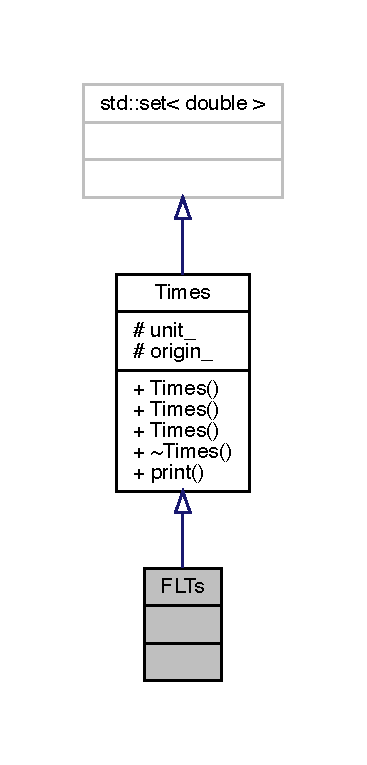
\includegraphics[width=179pt]{class_f_l_ts__inherit__graph}
\end{center}
\end{figure}


Collaboration diagram for F\+L\+Ts\+:
\nopagebreak
\begin{figure}[H]
\begin{center}
\leavevmode
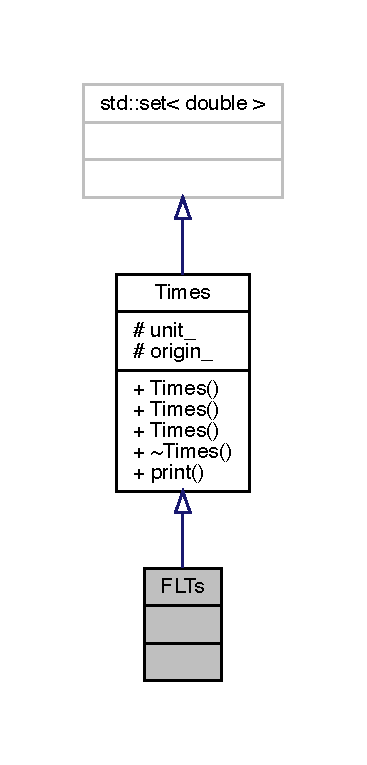
\includegraphics[width=179pt]{class_f_l_ts__coll__graph}
\end{center}
\end{figure}
\subsection*{Friends}
\begin{DoxyCompactItemize}
\item 
std\+::ostream \& \mbox{\hyperlink{class_f_l_ts_ae6eedde5f18b77e7a2922bc9a3f6b8bf}{operator$<$$<$}} (std\+::ostream \&os, \mbox{\hyperlink{class_f_l_ts}{F\+L\+Ts}} const \&obj)
\end{DoxyCompactItemize}
\subsection*{Additional Inherited Members}


\subsection{Friends And Related Function Documentation}
\mbox{\Hypertarget{class_f_l_ts_ae6eedde5f18b77e7a2922bc9a3f6b8bf}\label{class_f_l_ts_ae6eedde5f18b77e7a2922bc9a3f6b8bf}} 
\index{F\+L\+Ts@{F\+L\+Ts}!operator$<$$<$@{operator$<$$<$}}
\index{operator$<$$<$@{operator$<$$<$}!F\+L\+Ts@{F\+L\+Ts}}
\subsubsection{\texorpdfstring{operator$<$$<$}{operator<<}}
{\footnotesize\ttfamily std\+::ostream\& operator$<$$<$ (\begin{DoxyParamCaption}\item[{std\+::ostream \&}]{os,  }\item[{\mbox{\hyperlink{class_f_l_ts}{F\+L\+Ts}} const \&}]{obj }\end{DoxyParamCaption})\hspace{0.3cm}{\ttfamily [friend]}}



The documentation for this class was generated from the following files\+:\begin{DoxyCompactItemize}
\item 
\mbox{\hyperlink{_times_8h}{Times.\+h}}\item 
\mbox{\hyperlink{_times_8cpp}{Times.\+cpp}}\end{DoxyCompactItemize}

\hypertarget{class_forecasts}{}\section{Forecasts Class Reference}
\label{class_forecasts}\index{Forecasts@{Forecasts}}


{\ttfamily \#include $<$Forecasts.\+h$>$}



Inheritance diagram for Forecasts\+:
\nopagebreak
\begin{figure}[H]
\begin{center}
\leavevmode
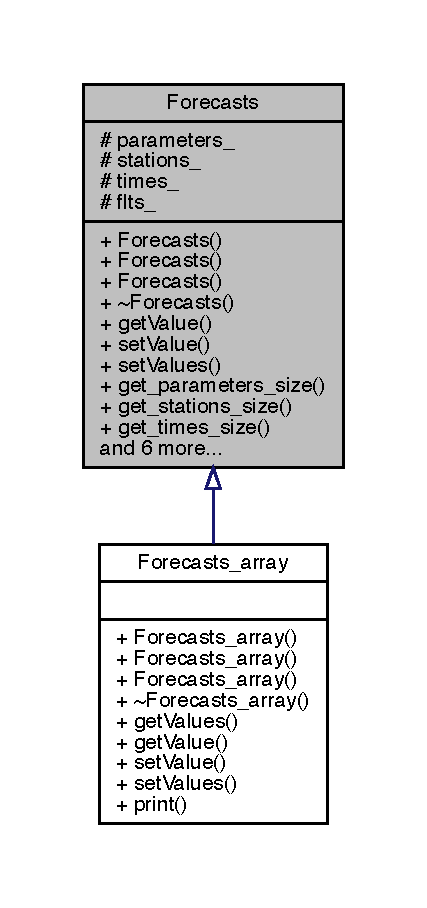
\includegraphics[width=205pt]{class_forecasts__inherit__graph}
\end{center}
\end{figure}


Collaboration diagram for Forecasts\+:
\nopagebreak
\begin{figure}[H]
\begin{center}
\leavevmode
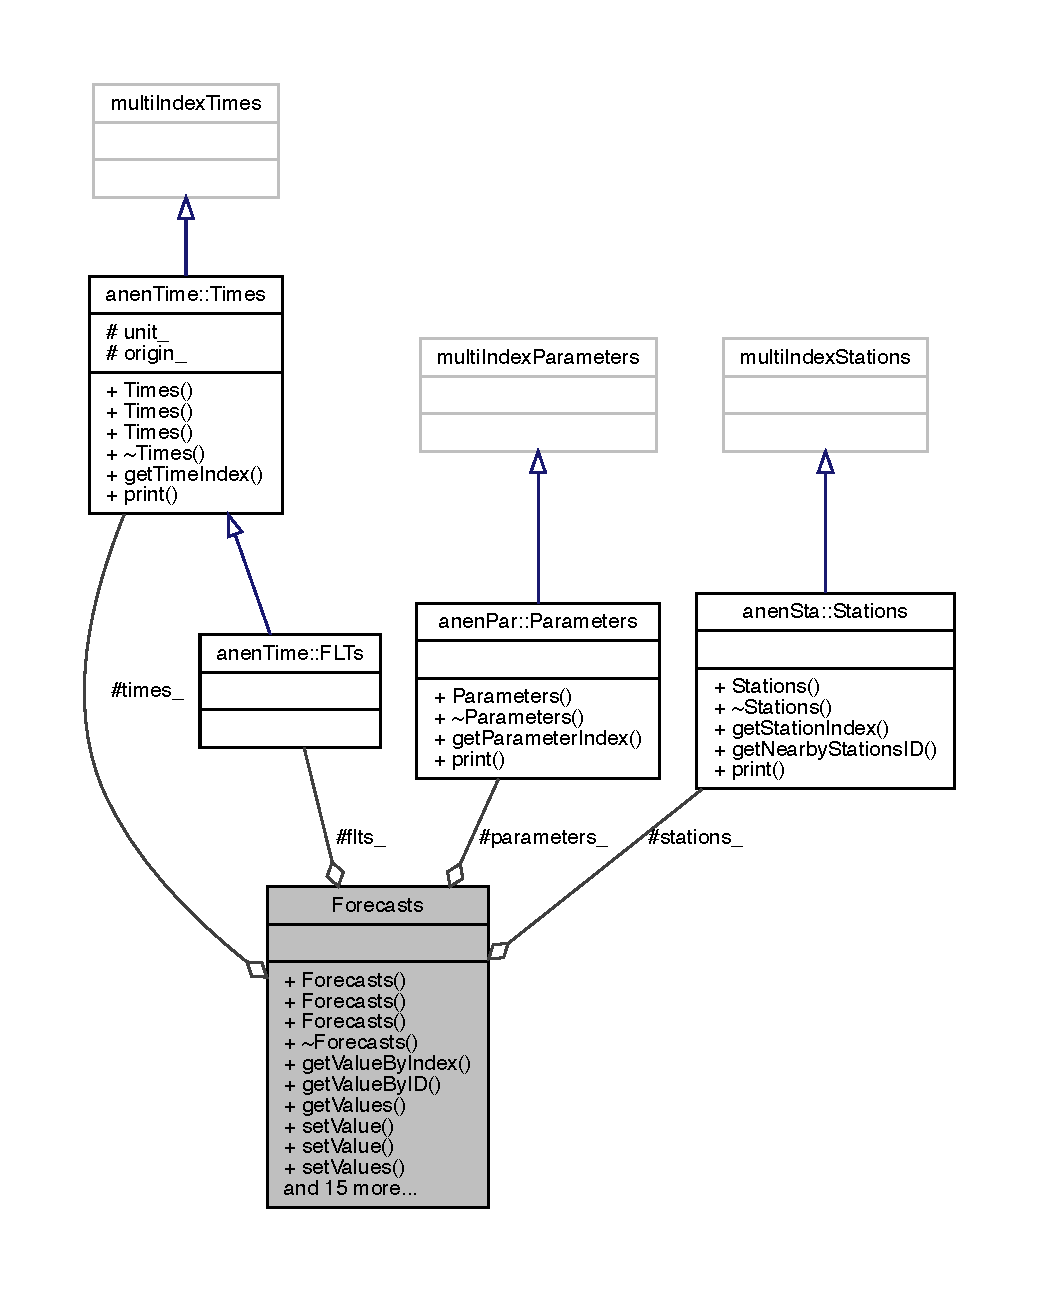
\includegraphics[width=350pt]{class_forecasts__coll__graph}
\end{center}
\end{figure}
\subsection*{Public Member Functions}
\begin{DoxyCompactItemize}
\item 
\mbox{\hyperlink{class_forecasts_a0e602a4bb37b4d6092f475da8c20ed27}{Forecasts}} ()=delete
\item 
\mbox{\hyperlink{class_forecasts_a6f47e34b9ae9bb9496149208e3246d65}{Forecasts}} (\mbox{\hyperlink{class_forecasts}{Forecasts}} const \&)=delete
\item 
\mbox{\hyperlink{class_forecasts_a9a7ee86b148267a59aec821e44d5f7d9}{Forecasts}} (\mbox{\hyperlink{class_parameters}{Parameters}}, \mbox{\hyperlink{class_stations}{Stations}}, \mbox{\hyperlink{class_times}{Times}}, \mbox{\hyperlink{class_f_l_ts}{F\+L\+Ts}})
\item 
virtual \mbox{\hyperlink{class_forecasts_a340fd19812d62efc334fe4d23ff8dcd2}{$\sim$\+Forecasts}} ()
\item 
virtual double \mbox{\hyperlink{class_forecasts_a07a51e97b54a5c42d197fb4804ee43bc}{get\+Value}} (std\+::size\+\_\+t parameter\+\_\+\+ID, std\+::size\+\_\+t station\+\_\+\+ID, double timestamp, double flt) const =0
\item 
virtual bool \mbox{\hyperlink{class_forecasts_ac3ba966466c340deaecf83fa239bef6d}{set\+Value}} (double, std\+::size\+\_\+t parameter\+\_\+\+ID, std\+::size\+\_\+t station\+\_\+\+ID, double timestamp, double flt)=0
\item 
virtual bool \mbox{\hyperlink{class_forecasts_a2f249a4ec8571dcf2cfc23f06b942ad9}{set\+Values}} (const std\+::vector$<$ double $>$ \&vals)=0
\item 
std\+::size\+\_\+t \mbox{\hyperlink{class_forecasts_a445efc69dce930a1c308d17289466e68}{get\+\_\+parameters\+\_\+size}} () const
\item 
std\+::size\+\_\+t \mbox{\hyperlink{class_forecasts_abec05f11da96ef797e741178b2a7335c}{get\+\_\+stations\+\_\+size}} () const
\item 
std\+::size\+\_\+t \mbox{\hyperlink{class_forecasts_a267f33699ada17b57e2c05a25a01d1c3}{get\+\_\+times\+\_\+size}} () const
\item 
std\+::size\+\_\+t \mbox{\hyperlink{class_forecasts_a5cea0e9e7f39a95a26878fefc0c29b7b}{get\+\_\+flts\+\_\+size}} () const
\item 
\mbox{\hyperlink{class_parameters}{Parameters}} const  \& \mbox{\hyperlink{class_forecasts_a3f3bfa7ff06856f8e965fd440fa2f4ae}{get\+Parameters}} () const
\item 
\mbox{\hyperlink{class_stations}{Stations}} const  \& \mbox{\hyperlink{class_forecasts_a3db4c9546c88683586b606500a5e3c22}{get\+Stations}} () const
\item 
\mbox{\hyperlink{class_times}{Times}} const  \& \mbox{\hyperlink{class_forecasts_a269d0121cfb01a9f3299df572c7f83be}{get\+Times}} () const
\item 
\mbox{\hyperlink{class_f_l_ts}{F\+L\+Ts}} const  \& \mbox{\hyperlink{class_forecasts_aa791d0794da8090a572764665d43180f}{get\+F\+L\+Ts}} () const
\item 
virtual void \mbox{\hyperlink{class_forecasts_addb1f75f0dc6833c466453c51256812c}{print}} (std\+::ostream \&) const
\end{DoxyCompactItemize}
\subsection*{Protected Attributes}
\begin{DoxyCompactItemize}
\item 
\mbox{\hyperlink{class_parameters}{Parameters}} \mbox{\hyperlink{class_forecasts_a3705673d34a2f6468659955fb3d28abb}{parameters\+\_\+}}
\item 
\mbox{\hyperlink{class_stations}{Stations}} \mbox{\hyperlink{class_forecasts_a5557d3b6c0700d6da88d2610f95287ab}{stations\+\_\+}}
\item 
\mbox{\hyperlink{class_times}{Times}} \mbox{\hyperlink{class_forecasts_abe5747fb6460d05937ab95ff3b7f8b3f}{times\+\_\+}}
\item 
\mbox{\hyperlink{class_f_l_ts}{F\+L\+Ts}} \mbox{\hyperlink{class_forecasts_a5bbcb6eb5d291718f8f91e576827518b}{flts\+\_\+}}
\end{DoxyCompactItemize}
\subsection*{Friends}
\begin{DoxyCompactItemize}
\item 
std\+::ostream \& \mbox{\hyperlink{class_forecasts_a42c14120042eae287169092654f5b6c8}{operator$<$$<$}} (std\+::ostream \&, \mbox{\hyperlink{class_forecasts}{Forecasts}} const \&)
\end{DoxyCompactItemize}


\subsection{Constructor \& Destructor Documentation}
\mbox{\Hypertarget{class_forecasts_a0e602a4bb37b4d6092f475da8c20ed27}\label{class_forecasts_a0e602a4bb37b4d6092f475da8c20ed27}} 
\index{Forecasts@{Forecasts}!Forecasts@{Forecasts}}
\index{Forecasts@{Forecasts}!Forecasts@{Forecasts}}
\subsubsection{\texorpdfstring{Forecasts()}{Forecasts()}\hspace{0.1cm}{\footnotesize\ttfamily [1/3]}}
{\footnotesize\ttfamily Forecasts\+::\+Forecasts (\begin{DoxyParamCaption}{ }\end{DoxyParamCaption})\hspace{0.3cm}{\ttfamily [delete]}}

\mbox{\Hypertarget{class_forecasts_a6f47e34b9ae9bb9496149208e3246d65}\label{class_forecasts_a6f47e34b9ae9bb9496149208e3246d65}} 
\index{Forecasts@{Forecasts}!Forecasts@{Forecasts}}
\index{Forecasts@{Forecasts}!Forecasts@{Forecasts}}
\subsubsection{\texorpdfstring{Forecasts()}{Forecasts()}\hspace{0.1cm}{\footnotesize\ttfamily [2/3]}}
{\footnotesize\ttfamily Forecasts\+::\+Forecasts (\begin{DoxyParamCaption}\item[{\mbox{\hyperlink{class_forecasts}{Forecasts}} const \&}]{ }\end{DoxyParamCaption})\hspace{0.3cm}{\ttfamily [delete]}}

\mbox{\Hypertarget{class_forecasts_a9a7ee86b148267a59aec821e44d5f7d9}\label{class_forecasts_a9a7ee86b148267a59aec821e44d5f7d9}} 
\index{Forecasts@{Forecasts}!Forecasts@{Forecasts}}
\index{Forecasts@{Forecasts}!Forecasts@{Forecasts}}
\subsubsection{\texorpdfstring{Forecasts()}{Forecasts()}\hspace{0.1cm}{\footnotesize\ttfamily [3/3]}}
{\footnotesize\ttfamily Forecasts\+::\+Forecasts (\begin{DoxyParamCaption}\item[{\mbox{\hyperlink{class_parameters}{Parameters}}}]{parameters,  }\item[{\mbox{\hyperlink{class_stations}{Stations}}}]{stations,  }\item[{\mbox{\hyperlink{class_times}{Times}}}]{time,  }\item[{\mbox{\hyperlink{class_f_l_ts}{F\+L\+Ts}}}]{flt }\end{DoxyParamCaption})}

\mbox{\Hypertarget{class_forecasts_a340fd19812d62efc334fe4d23ff8dcd2}\label{class_forecasts_a340fd19812d62efc334fe4d23ff8dcd2}} 
\index{Forecasts@{Forecasts}!````~Forecasts@{$\sim$\+Forecasts}}
\index{````~Forecasts@{$\sim$\+Forecasts}!Forecasts@{Forecasts}}
\subsubsection{\texorpdfstring{$\sim$\+Forecasts()}{~Forecasts()}}
{\footnotesize\ttfamily Forecasts\+::$\sim$\+Forecasts (\begin{DoxyParamCaption}{ }\end{DoxyParamCaption})\hspace{0.3cm}{\ttfamily [virtual]}}



\subsection{Member Function Documentation}
\mbox{\Hypertarget{class_forecasts_a5cea0e9e7f39a95a26878fefc0c29b7b}\label{class_forecasts_a5cea0e9e7f39a95a26878fefc0c29b7b}} 
\index{Forecasts@{Forecasts}!get\+\_\+flts\+\_\+size@{get\+\_\+flts\+\_\+size}}
\index{get\+\_\+flts\+\_\+size@{get\+\_\+flts\+\_\+size}!Forecasts@{Forecasts}}
\subsubsection{\texorpdfstring{get\+\_\+flts\+\_\+size()}{get\_flts\_size()}}
{\footnotesize\ttfamily size\+\_\+t Forecasts\+::get\+\_\+flts\+\_\+size (\begin{DoxyParamCaption}{ }\end{DoxyParamCaption}) const}

\mbox{\Hypertarget{class_forecasts_a445efc69dce930a1c308d17289466e68}\label{class_forecasts_a445efc69dce930a1c308d17289466e68}} 
\index{Forecasts@{Forecasts}!get\+\_\+parameters\+\_\+size@{get\+\_\+parameters\+\_\+size}}
\index{get\+\_\+parameters\+\_\+size@{get\+\_\+parameters\+\_\+size}!Forecasts@{Forecasts}}
\subsubsection{\texorpdfstring{get\+\_\+parameters\+\_\+size()}{get\_parameters\_size()}}
{\footnotesize\ttfamily size\+\_\+t Forecasts\+::get\+\_\+parameters\+\_\+size (\begin{DoxyParamCaption}{ }\end{DoxyParamCaption}) const}

\mbox{\Hypertarget{class_forecasts_abec05f11da96ef797e741178b2a7335c}\label{class_forecasts_abec05f11da96ef797e741178b2a7335c}} 
\index{Forecasts@{Forecasts}!get\+\_\+stations\+\_\+size@{get\+\_\+stations\+\_\+size}}
\index{get\+\_\+stations\+\_\+size@{get\+\_\+stations\+\_\+size}!Forecasts@{Forecasts}}
\subsubsection{\texorpdfstring{get\+\_\+stations\+\_\+size()}{get\_stations\_size()}}
{\footnotesize\ttfamily size\+\_\+t Forecasts\+::get\+\_\+stations\+\_\+size (\begin{DoxyParamCaption}{ }\end{DoxyParamCaption}) const}

\mbox{\Hypertarget{class_forecasts_a267f33699ada17b57e2c05a25a01d1c3}\label{class_forecasts_a267f33699ada17b57e2c05a25a01d1c3}} 
\index{Forecasts@{Forecasts}!get\+\_\+times\+\_\+size@{get\+\_\+times\+\_\+size}}
\index{get\+\_\+times\+\_\+size@{get\+\_\+times\+\_\+size}!Forecasts@{Forecasts}}
\subsubsection{\texorpdfstring{get\+\_\+times\+\_\+size()}{get\_times\_size()}}
{\footnotesize\ttfamily size\+\_\+t Forecasts\+::get\+\_\+times\+\_\+size (\begin{DoxyParamCaption}{ }\end{DoxyParamCaption}) const}

\mbox{\Hypertarget{class_forecasts_aa791d0794da8090a572764665d43180f}\label{class_forecasts_aa791d0794da8090a572764665d43180f}} 
\index{Forecasts@{Forecasts}!get\+F\+L\+Ts@{get\+F\+L\+Ts}}
\index{get\+F\+L\+Ts@{get\+F\+L\+Ts}!Forecasts@{Forecasts}}
\subsubsection{\texorpdfstring{get\+F\+L\+Ts()}{getFLTs()}}
{\footnotesize\ttfamily \mbox{\hyperlink{class_f_l_ts}{F\+L\+Ts}} const  \& Forecasts\+::get\+F\+L\+Ts (\begin{DoxyParamCaption}{ }\end{DoxyParamCaption}) const}

\mbox{\Hypertarget{class_forecasts_a3f3bfa7ff06856f8e965fd440fa2f4ae}\label{class_forecasts_a3f3bfa7ff06856f8e965fd440fa2f4ae}} 
\index{Forecasts@{Forecasts}!get\+Parameters@{get\+Parameters}}
\index{get\+Parameters@{get\+Parameters}!Forecasts@{Forecasts}}
\subsubsection{\texorpdfstring{get\+Parameters()}{getParameters()}}
{\footnotesize\ttfamily \mbox{\hyperlink{class_parameters}{Parameters}} const  \& Forecasts\+::get\+Parameters (\begin{DoxyParamCaption}{ }\end{DoxyParamCaption}) const}

\mbox{\Hypertarget{class_forecasts_a3db4c9546c88683586b606500a5e3c22}\label{class_forecasts_a3db4c9546c88683586b606500a5e3c22}} 
\index{Forecasts@{Forecasts}!get\+Stations@{get\+Stations}}
\index{get\+Stations@{get\+Stations}!Forecasts@{Forecasts}}
\subsubsection{\texorpdfstring{get\+Stations()}{getStations()}}
{\footnotesize\ttfamily \mbox{\hyperlink{class_stations}{Stations}} const  \& Forecasts\+::get\+Stations (\begin{DoxyParamCaption}{ }\end{DoxyParamCaption}) const}

\mbox{\Hypertarget{class_forecasts_a269d0121cfb01a9f3299df572c7f83be}\label{class_forecasts_a269d0121cfb01a9f3299df572c7f83be}} 
\index{Forecasts@{Forecasts}!get\+Times@{get\+Times}}
\index{get\+Times@{get\+Times}!Forecasts@{Forecasts}}
\subsubsection{\texorpdfstring{get\+Times()}{getTimes()}}
{\footnotesize\ttfamily \mbox{\hyperlink{class_times}{Times}} const  \& Forecasts\+::get\+Times (\begin{DoxyParamCaption}{ }\end{DoxyParamCaption}) const}

\mbox{\Hypertarget{class_forecasts_a07a51e97b54a5c42d197fb4804ee43bc}\label{class_forecasts_a07a51e97b54a5c42d197fb4804ee43bc}} 
\index{Forecasts@{Forecasts}!get\+Value@{get\+Value}}
\index{get\+Value@{get\+Value}!Forecasts@{Forecasts}}
\subsubsection{\texorpdfstring{get\+Value()}{getValue()}}
{\footnotesize\ttfamily virtual double Forecasts\+::get\+Value (\begin{DoxyParamCaption}\item[{std\+::size\+\_\+t}]{parameter\+\_\+\+ID,  }\item[{std\+::size\+\_\+t}]{station\+\_\+\+ID,  }\item[{double}]{timestamp,  }\item[{double}]{flt }\end{DoxyParamCaption}) const\hspace{0.3cm}{\ttfamily [pure virtual]}}



Implemented in \mbox{\hyperlink{class_forecasts__array_a38f7b890af0947e0d2022ce5bc5bb514}{Forecasts\+\_\+array}}.

\mbox{\Hypertarget{class_forecasts_addb1f75f0dc6833c466453c51256812c}\label{class_forecasts_addb1f75f0dc6833c466453c51256812c}} 
\index{Forecasts@{Forecasts}!print@{print}}
\index{print@{print}!Forecasts@{Forecasts}}
\subsubsection{\texorpdfstring{print()}{print()}}
{\footnotesize\ttfamily void Forecasts\+::print (\begin{DoxyParamCaption}\item[{std\+::ostream \&}]{ }\end{DoxyParamCaption}) const\hspace{0.3cm}{\ttfamily [virtual]}}



Reimplemented in \mbox{\hyperlink{class_forecasts__array_a56985347f516340034b29dc4cdda87b1}{Forecasts\+\_\+array}}.

\mbox{\Hypertarget{class_forecasts_ac3ba966466c340deaecf83fa239bef6d}\label{class_forecasts_ac3ba966466c340deaecf83fa239bef6d}} 
\index{Forecasts@{Forecasts}!set\+Value@{set\+Value}}
\index{set\+Value@{set\+Value}!Forecasts@{Forecasts}}
\subsubsection{\texorpdfstring{set\+Value()}{setValue()}}
{\footnotesize\ttfamily virtual bool Forecasts\+::set\+Value (\begin{DoxyParamCaption}\item[{double}]{,  }\item[{std\+::size\+\_\+t}]{parameter\+\_\+\+ID,  }\item[{std\+::size\+\_\+t}]{station\+\_\+\+ID,  }\item[{double}]{timestamp,  }\item[{double}]{flt }\end{DoxyParamCaption})\hspace{0.3cm}{\ttfamily [pure virtual]}}



Implemented in \mbox{\hyperlink{class_forecasts__array_a3b5557b58352d846c4fddc095f87589d}{Forecasts\+\_\+array}}.

\mbox{\Hypertarget{class_forecasts_a2f249a4ec8571dcf2cfc23f06b942ad9}\label{class_forecasts_a2f249a4ec8571dcf2cfc23f06b942ad9}} 
\index{Forecasts@{Forecasts}!set\+Values@{set\+Values}}
\index{set\+Values@{set\+Values}!Forecasts@{Forecasts}}
\subsubsection{\texorpdfstring{set\+Values()}{setValues()}}
{\footnotesize\ttfamily virtual bool Forecasts\+::set\+Values (\begin{DoxyParamCaption}\item[{const std\+::vector$<$ double $>$ \&}]{vals }\end{DoxyParamCaption})\hspace{0.3cm}{\ttfamily [pure virtual]}}

Sets data values from a vector.


\begin{DoxyParams}{Parameters}
{\em vals} & An std\+::vector$<$double$>$ object \\
\hline
\end{DoxyParams}
\begin{DoxyReturn}{Returns}
Returns true if succeed setting values. 
\end{DoxyReturn}


Implemented in \mbox{\hyperlink{class_forecasts__array_aba3f3632244ddb18c0b8a3fa0ee86981}{Forecasts\+\_\+array}}.



\subsection{Friends And Related Function Documentation}
\mbox{\Hypertarget{class_forecasts_a42c14120042eae287169092654f5b6c8}\label{class_forecasts_a42c14120042eae287169092654f5b6c8}} 
\index{Forecasts@{Forecasts}!operator$<$$<$@{operator$<$$<$}}
\index{operator$<$$<$@{operator$<$$<$}!Forecasts@{Forecasts}}
\subsubsection{\texorpdfstring{operator$<$$<$}{operator<<}}
{\footnotesize\ttfamily std\+::ostream\& operator$<$$<$ (\begin{DoxyParamCaption}\item[{std\+::ostream \&}]{,  }\item[{\mbox{\hyperlink{class_forecasts}{Forecasts}} const \&}]{ }\end{DoxyParamCaption})\hspace{0.3cm}{\ttfamily [friend]}}



\subsection{Member Data Documentation}
\mbox{\Hypertarget{class_forecasts_a5bbcb6eb5d291718f8f91e576827518b}\label{class_forecasts_a5bbcb6eb5d291718f8f91e576827518b}} 
\index{Forecasts@{Forecasts}!flts\+\_\+@{flts\+\_\+}}
\index{flts\+\_\+@{flts\+\_\+}!Forecasts@{Forecasts}}
\subsubsection{\texorpdfstring{flts\+\_\+}{flts\_}}
{\footnotesize\ttfamily \mbox{\hyperlink{class_f_l_ts}{F\+L\+Ts}} Forecasts\+::flts\+\_\+\hspace{0.3cm}{\ttfamily [protected]}}

\mbox{\Hypertarget{class_forecasts_a3705673d34a2f6468659955fb3d28abb}\label{class_forecasts_a3705673d34a2f6468659955fb3d28abb}} 
\index{Forecasts@{Forecasts}!parameters\+\_\+@{parameters\+\_\+}}
\index{parameters\+\_\+@{parameters\+\_\+}!Forecasts@{Forecasts}}
\subsubsection{\texorpdfstring{parameters\+\_\+}{parameters\_}}
{\footnotesize\ttfamily \mbox{\hyperlink{class_parameters}{Parameters}} Forecasts\+::parameters\+\_\+\hspace{0.3cm}{\ttfamily [protected]}}

\mbox{\Hypertarget{class_forecasts_a5557d3b6c0700d6da88d2610f95287ab}\label{class_forecasts_a5557d3b6c0700d6da88d2610f95287ab}} 
\index{Forecasts@{Forecasts}!stations\+\_\+@{stations\+\_\+}}
\index{stations\+\_\+@{stations\+\_\+}!Forecasts@{Forecasts}}
\subsubsection{\texorpdfstring{stations\+\_\+}{stations\_}}
{\footnotesize\ttfamily \mbox{\hyperlink{class_stations}{Stations}} Forecasts\+::stations\+\_\+\hspace{0.3cm}{\ttfamily [protected]}}

\mbox{\Hypertarget{class_forecasts_abe5747fb6460d05937ab95ff3b7f8b3f}\label{class_forecasts_abe5747fb6460d05937ab95ff3b7f8b3f}} 
\index{Forecasts@{Forecasts}!times\+\_\+@{times\+\_\+}}
\index{times\+\_\+@{times\+\_\+}!Forecasts@{Forecasts}}
\subsubsection{\texorpdfstring{times\+\_\+}{times\_}}
{\footnotesize\ttfamily \mbox{\hyperlink{class_times}{Times}} Forecasts\+::times\+\_\+\hspace{0.3cm}{\ttfamily [protected]}}



The documentation for this class was generated from the following files\+:\begin{DoxyCompactItemize}
\item 
\mbox{\hyperlink{_forecasts_8h}{Forecasts.\+h}}\item 
\mbox{\hyperlink{_forecasts_8cpp}{Forecasts.\+cpp}}\end{DoxyCompactItemize}

\hypertarget{class_forecasts__array}{}\section{Forecasts\+\_\+array Class Reference}
\label{class_forecasts__array}\index{Forecasts\+\_\+array@{Forecasts\+\_\+array}}


{\ttfamily \#include $<$Forecasts.\+h$>$}



Inheritance diagram for Forecasts\+\_\+array\+:
\nopagebreak
\begin{figure}[H]
\begin{center}
\leavevmode
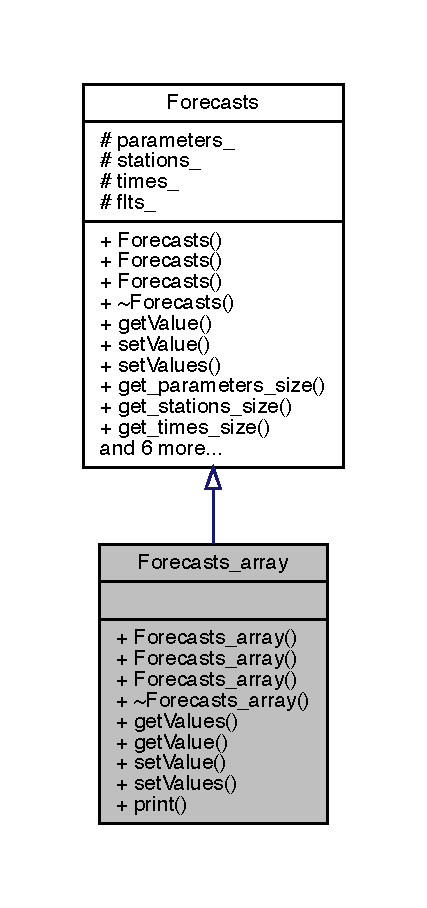
\includegraphics[width=205pt]{class_forecasts__array__inherit__graph}
\end{center}
\end{figure}


Collaboration diagram for Forecasts\+\_\+array\+:
\nopagebreak
\begin{figure}[H]
\begin{center}
\leavevmode
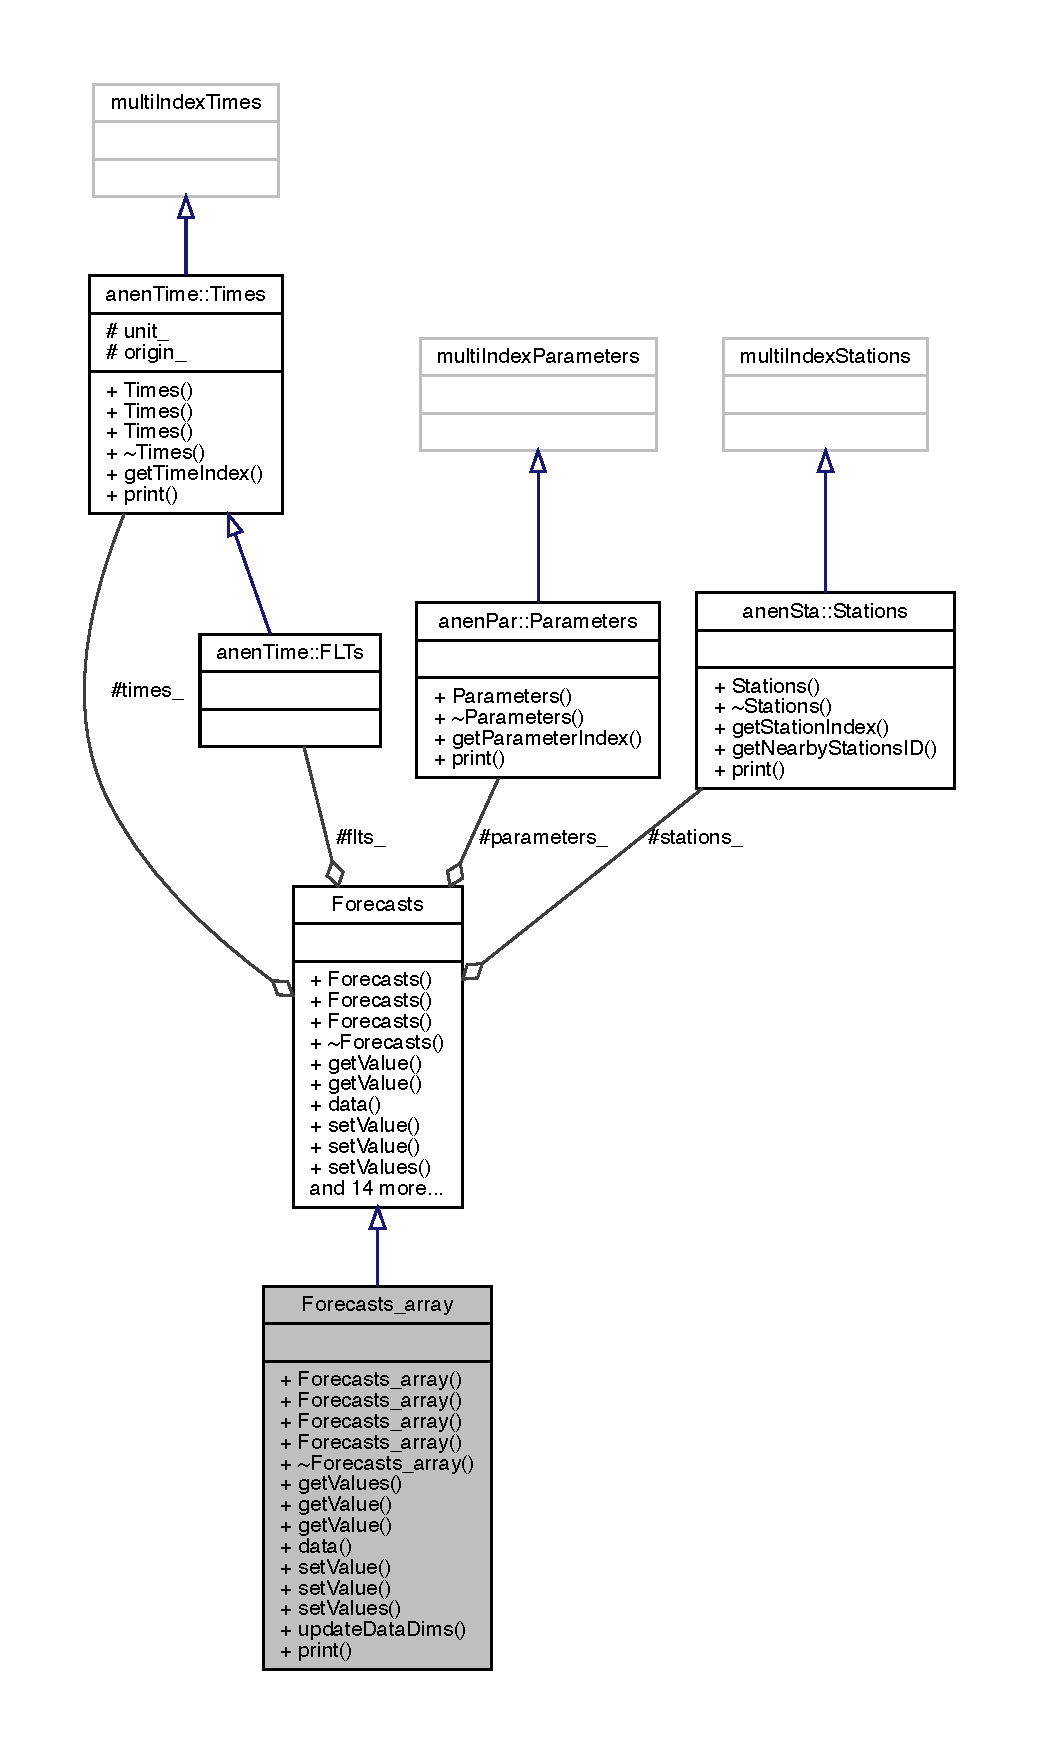
\includegraphics[height=550pt]{class_forecasts__array__coll__graph}
\end{center}
\end{figure}
\subsection*{Public Member Functions}
\begin{DoxyCompactItemize}
\item 
\mbox{\hyperlink{class_forecasts__array_a0158e2c3e0b874c81131cd61d6184ee6}{Forecasts\+\_\+array}} ()=delete
\item 
\mbox{\hyperlink{class_forecasts__array_a46a39594c6bc4f9b08ef3ff752147695}{Forecasts\+\_\+array}} (const \mbox{\hyperlink{class_forecasts__array}{Forecasts\+\_\+array}} \&rhs)=delete
\item 
\mbox{\hyperlink{class_forecasts__array_a248f861bf586b980c61b25cfce16a3c4}{Forecasts\+\_\+array}} (\mbox{\hyperlink{class_parameters}{Parameters}}, \mbox{\hyperlink{class_stations}{Stations}}, \mbox{\hyperlink{class_times}{Times}}, \mbox{\hyperlink{class_f_l_ts}{F\+L\+Ts}})
\item 
virtual \mbox{\hyperlink{class_forecasts__array_a7e13cb82b1ab76a45946cff992c7fff4}{$\sim$\+Forecasts\+\_\+array}} ()
\item 
\mbox{\hyperlink{class_array4_d}{Array4D}} const  \& \mbox{\hyperlink{class_forecasts__array_afd9f8bb1e1736bf3665073d95ae5ef8c}{get\+Values}} () const
\item 
double \mbox{\hyperlink{class_forecasts__array_a38f7b890af0947e0d2022ce5bc5bb514}{get\+Value}} (std\+::size\+\_\+t parameter\+\_\+\+ID, std\+::size\+\_\+t station\+\_\+\+ID, double timestamp, double flt) const override
\item 
bool \mbox{\hyperlink{class_forecasts__array_a3b5557b58352d846c4fddc095f87589d}{set\+Value}} (double, std\+::size\+\_\+t parameter\+\_\+\+ID, std\+::size\+\_\+t station\+\_\+\+ID, double timestamp, double flt) override
\item 
bool \mbox{\hyperlink{class_forecasts__array_aba3f3632244ddb18c0b8a3fa0ee86981}{set\+Values}} (const std\+::vector$<$ double $>$ \&vals) override
\item 
void \mbox{\hyperlink{class_forecasts__array_a56985347f516340034b29dc4cdda87b1}{print}} (std\+::ostream \&) const override
\end{DoxyCompactItemize}
\subsection*{Friends}
\begin{DoxyCompactItemize}
\item 
std\+::ostream \& \mbox{\hyperlink{class_forecasts__array_a6bde933a6e00ad1328f834e4f5d98606}{operator$<$$<$}} (std\+::ostream \&, const \mbox{\hyperlink{class_forecasts__array}{Forecasts\+\_\+array}} \&)
\end{DoxyCompactItemize}
\subsection*{Additional Inherited Members}


\subsection{Constructor \& Destructor Documentation}
\mbox{\Hypertarget{class_forecasts__array_a0158e2c3e0b874c81131cd61d6184ee6}\label{class_forecasts__array_a0158e2c3e0b874c81131cd61d6184ee6}} 
\index{Forecasts\+\_\+array@{Forecasts\+\_\+array}!Forecasts\+\_\+array@{Forecasts\+\_\+array}}
\index{Forecasts\+\_\+array@{Forecasts\+\_\+array}!Forecasts\+\_\+array@{Forecasts\+\_\+array}}
\subsubsection{\texorpdfstring{Forecasts\+\_\+array()}{Forecasts\_array()}\hspace{0.1cm}{\footnotesize\ttfamily [1/3]}}
{\footnotesize\ttfamily Forecasts\+\_\+array\+::\+Forecasts\+\_\+array (\begin{DoxyParamCaption}{ }\end{DoxyParamCaption})\hspace{0.3cm}{\ttfamily [delete]}}

\mbox{\Hypertarget{class_forecasts__array_a46a39594c6bc4f9b08ef3ff752147695}\label{class_forecasts__array_a46a39594c6bc4f9b08ef3ff752147695}} 
\index{Forecasts\+\_\+array@{Forecasts\+\_\+array}!Forecasts\+\_\+array@{Forecasts\+\_\+array}}
\index{Forecasts\+\_\+array@{Forecasts\+\_\+array}!Forecasts\+\_\+array@{Forecasts\+\_\+array}}
\subsubsection{\texorpdfstring{Forecasts\+\_\+array()}{Forecasts\_array()}\hspace{0.1cm}{\footnotesize\ttfamily [2/3]}}
{\footnotesize\ttfamily Forecasts\+\_\+array\+::\+Forecasts\+\_\+array (\begin{DoxyParamCaption}\item[{const \mbox{\hyperlink{class_forecasts__array}{Forecasts\+\_\+array}} \&}]{rhs }\end{DoxyParamCaption})\hspace{0.3cm}{\ttfamily [delete]}}

\mbox{\Hypertarget{class_forecasts__array_a248f861bf586b980c61b25cfce16a3c4}\label{class_forecasts__array_a248f861bf586b980c61b25cfce16a3c4}} 
\index{Forecasts\+\_\+array@{Forecasts\+\_\+array}!Forecasts\+\_\+array@{Forecasts\+\_\+array}}
\index{Forecasts\+\_\+array@{Forecasts\+\_\+array}!Forecasts\+\_\+array@{Forecasts\+\_\+array}}
\subsubsection{\texorpdfstring{Forecasts\+\_\+array()}{Forecasts\_array()}\hspace{0.1cm}{\footnotesize\ttfamily [3/3]}}
{\footnotesize\ttfamily Forecasts\+\_\+array\+::\+Forecasts\+\_\+array (\begin{DoxyParamCaption}\item[{\mbox{\hyperlink{class_parameters}{Parameters}}}]{parameters,  }\item[{\mbox{\hyperlink{class_stations}{Stations}}}]{stations,  }\item[{\mbox{\hyperlink{class_times}{Times}}}]{time,  }\item[{\mbox{\hyperlink{class_f_l_ts}{F\+L\+Ts}}}]{flt }\end{DoxyParamCaption})}

\mbox{\Hypertarget{class_forecasts__array_a7e13cb82b1ab76a45946cff992c7fff4}\label{class_forecasts__array_a7e13cb82b1ab76a45946cff992c7fff4}} 
\index{Forecasts\+\_\+array@{Forecasts\+\_\+array}!````~Forecasts\+\_\+array@{$\sim$\+Forecasts\+\_\+array}}
\index{````~Forecasts\+\_\+array@{$\sim$\+Forecasts\+\_\+array}!Forecasts\+\_\+array@{Forecasts\+\_\+array}}
\subsubsection{\texorpdfstring{$\sim$\+Forecasts\+\_\+array()}{~Forecasts\_array()}}
{\footnotesize\ttfamily Forecasts\+\_\+array\+::$\sim$\+Forecasts\+\_\+array (\begin{DoxyParamCaption}{ }\end{DoxyParamCaption})\hspace{0.3cm}{\ttfamily [virtual]}}



\subsection{Member Function Documentation}
\mbox{\Hypertarget{class_forecasts__array_a38f7b890af0947e0d2022ce5bc5bb514}\label{class_forecasts__array_a38f7b890af0947e0d2022ce5bc5bb514}} 
\index{Forecasts\+\_\+array@{Forecasts\+\_\+array}!get\+Value@{get\+Value}}
\index{get\+Value@{get\+Value}!Forecasts\+\_\+array@{Forecasts\+\_\+array}}
\subsubsection{\texorpdfstring{get\+Value()}{getValue()}}
{\footnotesize\ttfamily double Forecasts\+\_\+array\+::get\+Value (\begin{DoxyParamCaption}\item[{std\+::size\+\_\+t}]{parameter\+\_\+\+ID,  }\item[{std\+::size\+\_\+t}]{station\+\_\+\+ID,  }\item[{double}]{timestamp,  }\item[{double}]{flt }\end{DoxyParamCaption}) const\hspace{0.3cm}{\ttfamily [override]}, {\ttfamily [virtual]}}



Implements \mbox{\hyperlink{class_forecasts_a07a51e97b54a5c42d197fb4804ee43bc}{Forecasts}}.

\mbox{\Hypertarget{class_forecasts__array_afd9f8bb1e1736bf3665073d95ae5ef8c}\label{class_forecasts__array_afd9f8bb1e1736bf3665073d95ae5ef8c}} 
\index{Forecasts\+\_\+array@{Forecasts\+\_\+array}!get\+Values@{get\+Values}}
\index{get\+Values@{get\+Values}!Forecasts\+\_\+array@{Forecasts\+\_\+array}}
\subsubsection{\texorpdfstring{get\+Values()}{getValues()}}
{\footnotesize\ttfamily \mbox{\hyperlink{class_array4_d}{Array4D}} const  \& Forecasts\+\_\+array\+::get\+Values (\begin{DoxyParamCaption}{ }\end{DoxyParamCaption}) const}

\mbox{\Hypertarget{class_forecasts__array_a56985347f516340034b29dc4cdda87b1}\label{class_forecasts__array_a56985347f516340034b29dc4cdda87b1}} 
\index{Forecasts\+\_\+array@{Forecasts\+\_\+array}!print@{print}}
\index{print@{print}!Forecasts\+\_\+array@{Forecasts\+\_\+array}}
\subsubsection{\texorpdfstring{print()}{print()}}
{\footnotesize\ttfamily void Forecasts\+\_\+array\+::print (\begin{DoxyParamCaption}\item[{std\+::ostream \&}]{ }\end{DoxyParamCaption}) const\hspace{0.3cm}{\ttfamily [override]}, {\ttfamily [virtual]}}



Reimplemented from \mbox{\hyperlink{class_forecasts_addb1f75f0dc6833c466453c51256812c}{Forecasts}}.

\mbox{\Hypertarget{class_forecasts__array_a3b5557b58352d846c4fddc095f87589d}\label{class_forecasts__array_a3b5557b58352d846c4fddc095f87589d}} 
\index{Forecasts\+\_\+array@{Forecasts\+\_\+array}!set\+Value@{set\+Value}}
\index{set\+Value@{set\+Value}!Forecasts\+\_\+array@{Forecasts\+\_\+array}}
\subsubsection{\texorpdfstring{set\+Value()}{setValue()}}
{\footnotesize\ttfamily bool Forecasts\+\_\+array\+::set\+Value (\begin{DoxyParamCaption}\item[{double}]{,  }\item[{std\+::size\+\_\+t}]{parameter\+\_\+\+ID,  }\item[{std\+::size\+\_\+t}]{station\+\_\+\+ID,  }\item[{double}]{timestamp,  }\item[{double}]{flt }\end{DoxyParamCaption})\hspace{0.3cm}{\ttfamily [override]}, {\ttfamily [virtual]}}



Implements \mbox{\hyperlink{class_forecasts_ac3ba966466c340deaecf83fa239bef6d}{Forecasts}}.

\mbox{\Hypertarget{class_forecasts__array_aba3f3632244ddb18c0b8a3fa0ee86981}\label{class_forecasts__array_aba3f3632244ddb18c0b8a3fa0ee86981}} 
\index{Forecasts\+\_\+array@{Forecasts\+\_\+array}!set\+Values@{set\+Values}}
\index{set\+Values@{set\+Values}!Forecasts\+\_\+array@{Forecasts\+\_\+array}}
\subsubsection{\texorpdfstring{set\+Values()}{setValues()}}
{\footnotesize\ttfamily bool Forecasts\+\_\+array\+::set\+Values (\begin{DoxyParamCaption}\item[{const std\+::vector$<$ double $>$ \&}]{vals }\end{DoxyParamCaption})\hspace{0.3cm}{\ttfamily [override]}, {\ttfamily [virtual]}}

Sets data values from a vector.


\begin{DoxyParams}{Parameters}
{\em vals} & An std\+::vector$<$double$>$ object \\
\hline
\end{DoxyParams}
\begin{DoxyReturn}{Returns}
Returns true if succeed setting values. 
\end{DoxyReturn}


Implements \mbox{\hyperlink{class_forecasts_a2f249a4ec8571dcf2cfc23f06b942ad9}{Forecasts}}.



\subsection{Friends And Related Function Documentation}
\mbox{\Hypertarget{class_forecasts__array_a6bde933a6e00ad1328f834e4f5d98606}\label{class_forecasts__array_a6bde933a6e00ad1328f834e4f5d98606}} 
\index{Forecasts\+\_\+array@{Forecasts\+\_\+array}!operator$<$$<$@{operator$<$$<$}}
\index{operator$<$$<$@{operator$<$$<$}!Forecasts\+\_\+array@{Forecasts\+\_\+array}}
\subsubsection{\texorpdfstring{operator$<$$<$}{operator<<}}
{\footnotesize\ttfamily std\+::ostream\& operator$<$$<$ (\begin{DoxyParamCaption}\item[{std\+::ostream \&}]{,  }\item[{const \mbox{\hyperlink{class_forecasts__array}{Forecasts\+\_\+array}} \&}]{ }\end{DoxyParamCaption})\hspace{0.3cm}{\ttfamily [friend]}}



The documentation for this class was generated from the following files\+:\begin{DoxyCompactItemize}
\item 
\mbox{\hyperlink{_forecasts_8h}{Forecasts.\+h}}\item 
\mbox{\hyperlink{_forecasts_8cpp}{Forecasts.\+cpp}}\end{DoxyCompactItemize}

\hypertarget{class_observations}{}\section{Observations Class Reference}
\label{class_observations}\index{Observations@{Observations}}


{\ttfamily \#include $<$Observations.\+h$>$}



Inheritance diagram for Observations\+:
\nopagebreak
\begin{figure}[H]
\begin{center}
\leavevmode
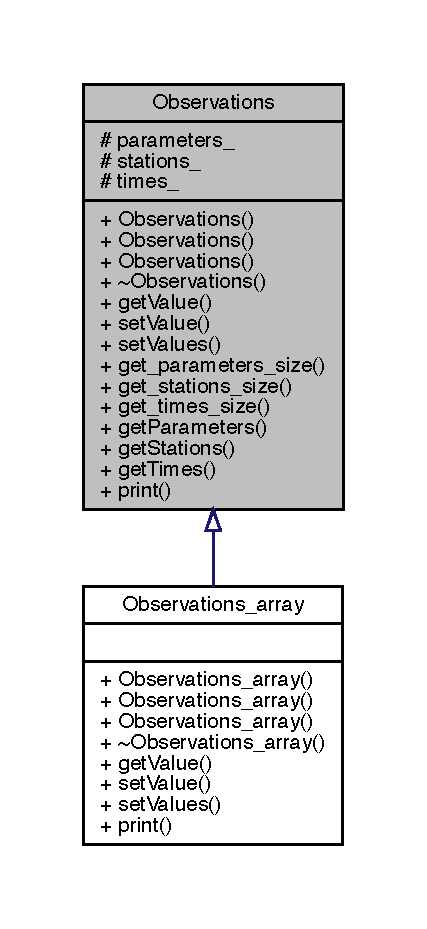
\includegraphics[width=205pt]{class_observations__inherit__graph}
\end{center}
\end{figure}


Collaboration diagram for Observations\+:
\nopagebreak
\begin{figure}[H]
\begin{center}
\leavevmode
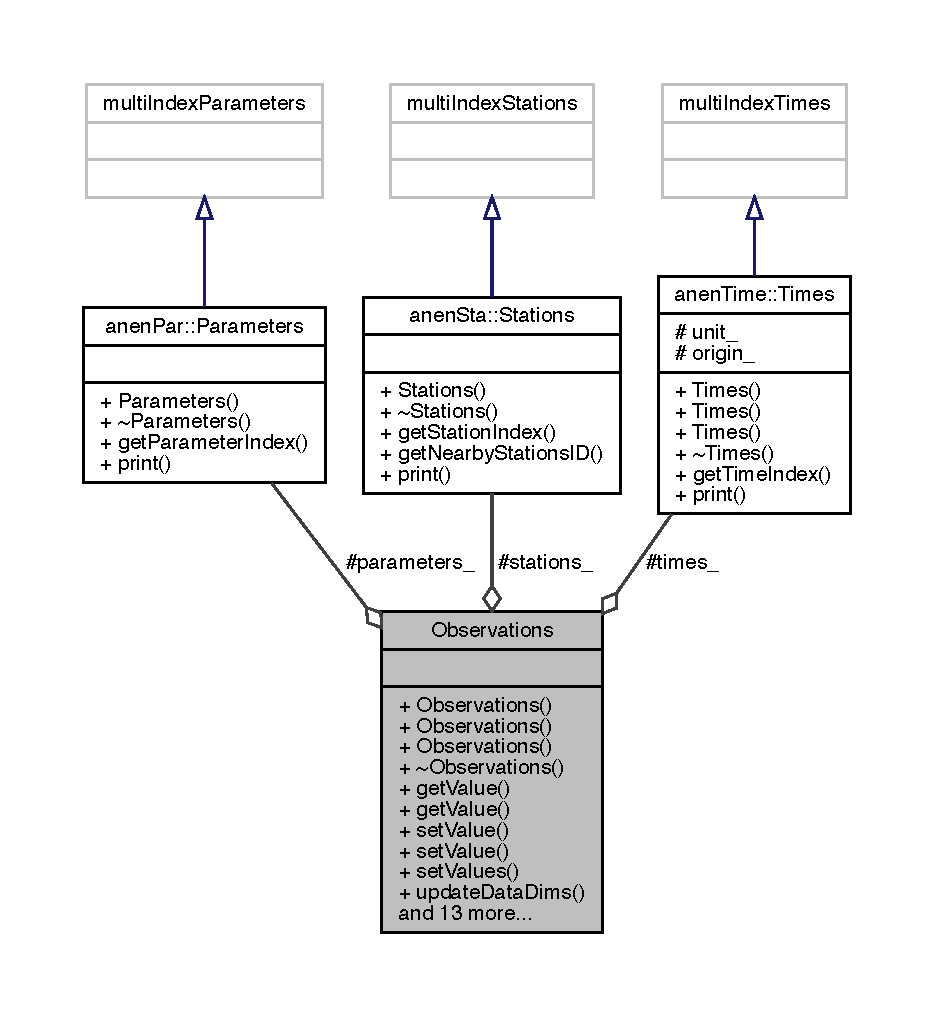
\includegraphics[width=350pt]{class_observations__coll__graph}
\end{center}
\end{figure}
\subsection*{Public Member Functions}
\begin{DoxyCompactItemize}
\item 
\mbox{\hyperlink{class_observations_ab5a998900064d3d0599e4548a6508d9f}{Observations}} ()=delete
\item 
\mbox{\hyperlink{class_observations_a579feccdac9c26226cf813ac8cf3521a}{Observations}} (const \mbox{\hyperlink{class_observations}{Observations}} \&orig)=delete
\item 
\mbox{\hyperlink{class_observations_a67aabf1b5bb51b8bcb9f6cf3df64f57d}{Observations}} (\mbox{\hyperlink{class_parameters}{Parameters}}, \mbox{\hyperlink{class_stations}{Stations}}, \mbox{\hyperlink{class_times}{Times}})
\item 
virtual \mbox{\hyperlink{class_observations_a8724b267cce796b0f77f8f2b9e4aaf1d}{$\sim$\+Observations}} ()
\item 
virtual double \mbox{\hyperlink{class_observations_ac5564bbf13e79d269407d1ecf567cd7f}{get\+Value}} (std\+::size\+\_\+t parameter\+\_\+\+ID, std\+::size\+\_\+t station\+\_\+\+ID, double timestamp) const =0
\item 
virtual bool \mbox{\hyperlink{class_observations_a359b5b8cd97cd43483444ca4fc188dff}{set\+Value}} (double, std\+::size\+\_\+t parameter\+\_\+\+ID, std\+::size\+\_\+t station\+\_\+\+ID, double timestamp)=0
\item 
virtual bool \mbox{\hyperlink{class_observations_a58e9bcf10981845ad5bf89b34cacdbd7}{set\+Values}} (const std\+::vector$<$ double $>$ \&vals)=0
\item 
std\+::size\+\_\+t \mbox{\hyperlink{class_observations_a4ae6818f6d01490eb14d63ce51a1d331}{get\+\_\+parameters\+\_\+size}} () const
\item 
std\+::size\+\_\+t \mbox{\hyperlink{class_observations_a30f67730e600545cf8cb9d7aed13bd33}{get\+\_\+stations\+\_\+size}} () const
\item 
std\+::size\+\_\+t \mbox{\hyperlink{class_observations_a352e34f7c278c86f54c69def24dabcd1}{get\+\_\+times\+\_\+size}} () const
\item 
\mbox{\hyperlink{class_parameters}{Parameters}} const  \& \mbox{\hyperlink{class_observations_a8401a31f796d79387603baeea5269b6b}{get\+Parameters}} () const
\item 
\mbox{\hyperlink{class_stations}{Stations}} const  \& \mbox{\hyperlink{class_observations_a3c9520bed358d0f2ce0a08b94c84b94c}{get\+Stations}} () const
\item 
\mbox{\hyperlink{class_times}{Times}} const  \& \mbox{\hyperlink{class_observations_a3d364631c280ad9c35238e781f63e75c}{get\+Times}} () const
\item 
virtual void \mbox{\hyperlink{class_observations_a523647c5ae644959f0ed583cd7b11aba}{print}} (std\+::ostream \&) const
\end{DoxyCompactItemize}
\subsection*{Protected Attributes}
\begin{DoxyCompactItemize}
\item 
\mbox{\hyperlink{class_parameters}{Parameters}} \mbox{\hyperlink{class_observations_ad86a168276ed510e2e56ac9a1e632848}{parameters\+\_\+}}
\item 
\mbox{\hyperlink{class_stations}{Stations}} \mbox{\hyperlink{class_observations_ad047997c0d421695f07be2edeef996ce}{stations\+\_\+}}
\item 
\mbox{\hyperlink{class_times}{Times}} \mbox{\hyperlink{class_observations_ab68b4495a78a2a30396cd42206d3e33c}{times\+\_\+}}
\end{DoxyCompactItemize}
\subsection*{Friends}
\begin{DoxyCompactItemize}
\item 
std\+::ostream \& \mbox{\hyperlink{class_observations_ad93ae2b52ac4bae27e3419d1545ee68f}{operator$<$$<$}} (std\+::ostream \&, const \mbox{\hyperlink{class_observations}{Observations}} \&)
\end{DoxyCompactItemize}


\subsection{Constructor \& Destructor Documentation}
\mbox{\Hypertarget{class_observations_ab5a998900064d3d0599e4548a6508d9f}\label{class_observations_ab5a998900064d3d0599e4548a6508d9f}} 
\index{Observations@{Observations}!Observations@{Observations}}
\index{Observations@{Observations}!Observations@{Observations}}
\subsubsection{\texorpdfstring{Observations()}{Observations()}\hspace{0.1cm}{\footnotesize\ttfamily [1/3]}}
{\footnotesize\ttfamily Observations\+::\+Observations (\begin{DoxyParamCaption}{ }\end{DoxyParamCaption})\hspace{0.3cm}{\ttfamily [delete]}}

\mbox{\Hypertarget{class_observations_a579feccdac9c26226cf813ac8cf3521a}\label{class_observations_a579feccdac9c26226cf813ac8cf3521a}} 
\index{Observations@{Observations}!Observations@{Observations}}
\index{Observations@{Observations}!Observations@{Observations}}
\subsubsection{\texorpdfstring{Observations()}{Observations()}\hspace{0.1cm}{\footnotesize\ttfamily [2/3]}}
{\footnotesize\ttfamily Observations\+::\+Observations (\begin{DoxyParamCaption}\item[{const \mbox{\hyperlink{class_observations}{Observations}} \&}]{orig }\end{DoxyParamCaption})\hspace{0.3cm}{\ttfamily [delete]}}

\mbox{\Hypertarget{class_observations_a67aabf1b5bb51b8bcb9f6cf3df64f57d}\label{class_observations_a67aabf1b5bb51b8bcb9f6cf3df64f57d}} 
\index{Observations@{Observations}!Observations@{Observations}}
\index{Observations@{Observations}!Observations@{Observations}}
\subsubsection{\texorpdfstring{Observations()}{Observations()}\hspace{0.1cm}{\footnotesize\ttfamily [3/3]}}
{\footnotesize\ttfamily Observations\+::\+Observations (\begin{DoxyParamCaption}\item[{\mbox{\hyperlink{class_parameters}{Parameters}}}]{parameters\+\_\+,  }\item[{\mbox{\hyperlink{class_stations}{Stations}}}]{stations\+\_\+,  }\item[{\mbox{\hyperlink{class_times}{Times}}}]{times\+\_\+ }\end{DoxyParamCaption})}

\mbox{\Hypertarget{class_observations_a8724b267cce796b0f77f8f2b9e4aaf1d}\label{class_observations_a8724b267cce796b0f77f8f2b9e4aaf1d}} 
\index{Observations@{Observations}!````~Observations@{$\sim$\+Observations}}
\index{````~Observations@{$\sim$\+Observations}!Observations@{Observations}}
\subsubsection{\texorpdfstring{$\sim$\+Observations()}{~Observations()}}
{\footnotesize\ttfamily Observations\+::$\sim$\+Observations (\begin{DoxyParamCaption}{ }\end{DoxyParamCaption})\hspace{0.3cm}{\ttfamily [virtual]}}



\subsection{Member Function Documentation}
\mbox{\Hypertarget{class_observations_a4ae6818f6d01490eb14d63ce51a1d331}\label{class_observations_a4ae6818f6d01490eb14d63ce51a1d331}} 
\index{Observations@{Observations}!get\+\_\+parameters\+\_\+size@{get\+\_\+parameters\+\_\+size}}
\index{get\+\_\+parameters\+\_\+size@{get\+\_\+parameters\+\_\+size}!Observations@{Observations}}
\subsubsection{\texorpdfstring{get\+\_\+parameters\+\_\+size()}{get\_parameters\_size()}}
{\footnotesize\ttfamily size\+\_\+t Observations\+::get\+\_\+parameters\+\_\+size (\begin{DoxyParamCaption}{ }\end{DoxyParamCaption}) const}

\mbox{\Hypertarget{class_observations_a30f67730e600545cf8cb9d7aed13bd33}\label{class_observations_a30f67730e600545cf8cb9d7aed13bd33}} 
\index{Observations@{Observations}!get\+\_\+stations\+\_\+size@{get\+\_\+stations\+\_\+size}}
\index{get\+\_\+stations\+\_\+size@{get\+\_\+stations\+\_\+size}!Observations@{Observations}}
\subsubsection{\texorpdfstring{get\+\_\+stations\+\_\+size()}{get\_stations\_size()}}
{\footnotesize\ttfamily size\+\_\+t Observations\+::get\+\_\+stations\+\_\+size (\begin{DoxyParamCaption}{ }\end{DoxyParamCaption}) const}

\mbox{\Hypertarget{class_observations_a352e34f7c278c86f54c69def24dabcd1}\label{class_observations_a352e34f7c278c86f54c69def24dabcd1}} 
\index{Observations@{Observations}!get\+\_\+times\+\_\+size@{get\+\_\+times\+\_\+size}}
\index{get\+\_\+times\+\_\+size@{get\+\_\+times\+\_\+size}!Observations@{Observations}}
\subsubsection{\texorpdfstring{get\+\_\+times\+\_\+size()}{get\_times\_size()}}
{\footnotesize\ttfamily size\+\_\+t Observations\+::get\+\_\+times\+\_\+size (\begin{DoxyParamCaption}{ }\end{DoxyParamCaption}) const}

\mbox{\Hypertarget{class_observations_a8401a31f796d79387603baeea5269b6b}\label{class_observations_a8401a31f796d79387603baeea5269b6b}} 
\index{Observations@{Observations}!get\+Parameters@{get\+Parameters}}
\index{get\+Parameters@{get\+Parameters}!Observations@{Observations}}
\subsubsection{\texorpdfstring{get\+Parameters()}{getParameters()}}
{\footnotesize\ttfamily \mbox{\hyperlink{class_parameters}{Parameters}} const  \& Observations\+::get\+Parameters (\begin{DoxyParamCaption}{ }\end{DoxyParamCaption}) const}

\mbox{\Hypertarget{class_observations_a3c9520bed358d0f2ce0a08b94c84b94c}\label{class_observations_a3c9520bed358d0f2ce0a08b94c84b94c}} 
\index{Observations@{Observations}!get\+Stations@{get\+Stations}}
\index{get\+Stations@{get\+Stations}!Observations@{Observations}}
\subsubsection{\texorpdfstring{get\+Stations()}{getStations()}}
{\footnotesize\ttfamily \mbox{\hyperlink{class_stations}{Stations}} const  \& Observations\+::get\+Stations (\begin{DoxyParamCaption}{ }\end{DoxyParamCaption}) const}

\mbox{\Hypertarget{class_observations_a3d364631c280ad9c35238e781f63e75c}\label{class_observations_a3d364631c280ad9c35238e781f63e75c}} 
\index{Observations@{Observations}!get\+Times@{get\+Times}}
\index{get\+Times@{get\+Times}!Observations@{Observations}}
\subsubsection{\texorpdfstring{get\+Times()}{getTimes()}}
{\footnotesize\ttfamily \mbox{\hyperlink{class_times}{Times}} const  \& Observations\+::get\+Times (\begin{DoxyParamCaption}{ }\end{DoxyParamCaption}) const}

\mbox{\Hypertarget{class_observations_ac5564bbf13e79d269407d1ecf567cd7f}\label{class_observations_ac5564bbf13e79d269407d1ecf567cd7f}} 
\index{Observations@{Observations}!get\+Value@{get\+Value}}
\index{get\+Value@{get\+Value}!Observations@{Observations}}
\subsubsection{\texorpdfstring{get\+Value()}{getValue()}}
{\footnotesize\ttfamily virtual double Observations\+::get\+Value (\begin{DoxyParamCaption}\item[{std\+::size\+\_\+t}]{parameter\+\_\+\+ID,  }\item[{std\+::size\+\_\+t}]{station\+\_\+\+ID,  }\item[{double}]{timestamp }\end{DoxyParamCaption}) const\hspace{0.3cm}{\ttfamily [pure virtual]}}



Implemented in \mbox{\hyperlink{class_observations__array_a33f2154b3fed9d488e06e8c92eecc4db}{Observations\+\_\+array}}.

\mbox{\Hypertarget{class_observations_a523647c5ae644959f0ed583cd7b11aba}\label{class_observations_a523647c5ae644959f0ed583cd7b11aba}} 
\index{Observations@{Observations}!print@{print}}
\index{print@{print}!Observations@{Observations}}
\subsubsection{\texorpdfstring{print()}{print()}}
{\footnotesize\ttfamily void Observations\+::print (\begin{DoxyParamCaption}\item[{std\+::ostream \&}]{ }\end{DoxyParamCaption}) const\hspace{0.3cm}{\ttfamily [virtual]}}



Reimplemented in \mbox{\hyperlink{class_observations__array_a2563545e5a38ec7e3ec09380c0b38855}{Observations\+\_\+array}}.

\mbox{\Hypertarget{class_observations_a359b5b8cd97cd43483444ca4fc188dff}\label{class_observations_a359b5b8cd97cd43483444ca4fc188dff}} 
\index{Observations@{Observations}!set\+Value@{set\+Value}}
\index{set\+Value@{set\+Value}!Observations@{Observations}}
\subsubsection{\texorpdfstring{set\+Value()}{setValue()}}
{\footnotesize\ttfamily virtual bool Observations\+::set\+Value (\begin{DoxyParamCaption}\item[{double}]{,  }\item[{std\+::size\+\_\+t}]{parameter\+\_\+\+ID,  }\item[{std\+::size\+\_\+t}]{station\+\_\+\+ID,  }\item[{double}]{timestamp }\end{DoxyParamCaption})\hspace{0.3cm}{\ttfamily [pure virtual]}}



Implemented in \mbox{\hyperlink{class_observations__array_a1708fe12a750cb68bb60782ab184605b}{Observations\+\_\+array}}.

\mbox{\Hypertarget{class_observations_a58e9bcf10981845ad5bf89b34cacdbd7}\label{class_observations_a58e9bcf10981845ad5bf89b34cacdbd7}} 
\index{Observations@{Observations}!set\+Values@{set\+Values}}
\index{set\+Values@{set\+Values}!Observations@{Observations}}
\subsubsection{\texorpdfstring{set\+Values()}{setValues()}}
{\footnotesize\ttfamily virtual bool Observations\+::set\+Values (\begin{DoxyParamCaption}\item[{const std\+::vector$<$ double $>$ \&}]{vals }\end{DoxyParamCaption})\hspace{0.3cm}{\ttfamily [pure virtual]}}

Sets data values from a vector.


\begin{DoxyParams}{Parameters}
{\em vals} & An std\+::vector$<$double$>$ object \\
\hline
\end{DoxyParams}
\begin{DoxyReturn}{Returns}
Returns true if succeed setting values. 
\end{DoxyReturn}


Implemented in \mbox{\hyperlink{class_observations__array_a59ee8d2a6b0d0158a3efa7c200c8ff43}{Observations\+\_\+array}}.



\subsection{Friends And Related Function Documentation}
\mbox{\Hypertarget{class_observations_ad93ae2b52ac4bae27e3419d1545ee68f}\label{class_observations_ad93ae2b52ac4bae27e3419d1545ee68f}} 
\index{Observations@{Observations}!operator$<$$<$@{operator$<$$<$}}
\index{operator$<$$<$@{operator$<$$<$}!Observations@{Observations}}
\subsubsection{\texorpdfstring{operator$<$$<$}{operator<<}}
{\footnotesize\ttfamily std\+::ostream\& operator$<$$<$ (\begin{DoxyParamCaption}\item[{std\+::ostream \&}]{,  }\item[{const \mbox{\hyperlink{class_observations}{Observations}} \&}]{ }\end{DoxyParamCaption})\hspace{0.3cm}{\ttfamily [friend]}}



\subsection{Member Data Documentation}
\mbox{\Hypertarget{class_observations_ad86a168276ed510e2e56ac9a1e632848}\label{class_observations_ad86a168276ed510e2e56ac9a1e632848}} 
\index{Observations@{Observations}!parameters\+\_\+@{parameters\+\_\+}}
\index{parameters\+\_\+@{parameters\+\_\+}!Observations@{Observations}}
\subsubsection{\texorpdfstring{parameters\+\_\+}{parameters\_}}
{\footnotesize\ttfamily \mbox{\hyperlink{class_parameters}{Parameters}} Observations\+::parameters\+\_\+\hspace{0.3cm}{\ttfamily [protected]}}

\mbox{\Hypertarget{class_observations_ad047997c0d421695f07be2edeef996ce}\label{class_observations_ad047997c0d421695f07be2edeef996ce}} 
\index{Observations@{Observations}!stations\+\_\+@{stations\+\_\+}}
\index{stations\+\_\+@{stations\+\_\+}!Observations@{Observations}}
\subsubsection{\texorpdfstring{stations\+\_\+}{stations\_}}
{\footnotesize\ttfamily \mbox{\hyperlink{class_stations}{Stations}} Observations\+::stations\+\_\+\hspace{0.3cm}{\ttfamily [protected]}}

\mbox{\Hypertarget{class_observations_ab68b4495a78a2a30396cd42206d3e33c}\label{class_observations_ab68b4495a78a2a30396cd42206d3e33c}} 
\index{Observations@{Observations}!times\+\_\+@{times\+\_\+}}
\index{times\+\_\+@{times\+\_\+}!Observations@{Observations}}
\subsubsection{\texorpdfstring{times\+\_\+}{times\_}}
{\footnotesize\ttfamily \mbox{\hyperlink{class_times}{Times}} Observations\+::times\+\_\+\hspace{0.3cm}{\ttfamily [protected]}}



The documentation for this class was generated from the following files\+:\begin{DoxyCompactItemize}
\item 
\mbox{\hyperlink{_observations_8h}{Observations.\+h}}\item 
\mbox{\hyperlink{_observations_8cpp}{Observations.\+cpp}}\end{DoxyCompactItemize}

\hypertarget{class_observations__array}{}\section{Observations\+\_\+array Class Reference}
\label{class_observations__array}\index{Observations\+\_\+array@{Observations\+\_\+array}}


{\ttfamily \#include $<$Observations.\+h$>$}



Inheritance diagram for Observations\+\_\+array\+:
\nopagebreak
\begin{figure}[H]
\begin{center}
\leavevmode
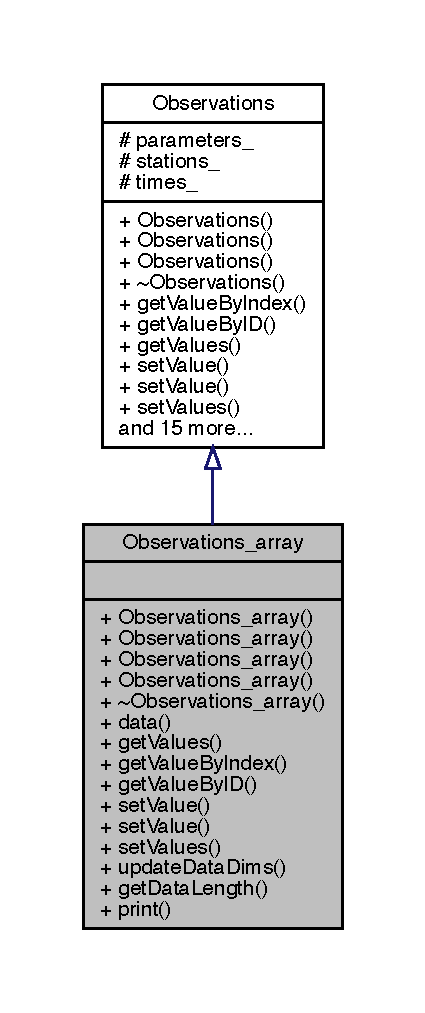
\includegraphics[width=205pt]{class_observations__array__inherit__graph}
\end{center}
\end{figure}


Collaboration diagram for Observations\+\_\+array\+:
\nopagebreak
\begin{figure}[H]
\begin{center}
\leavevmode
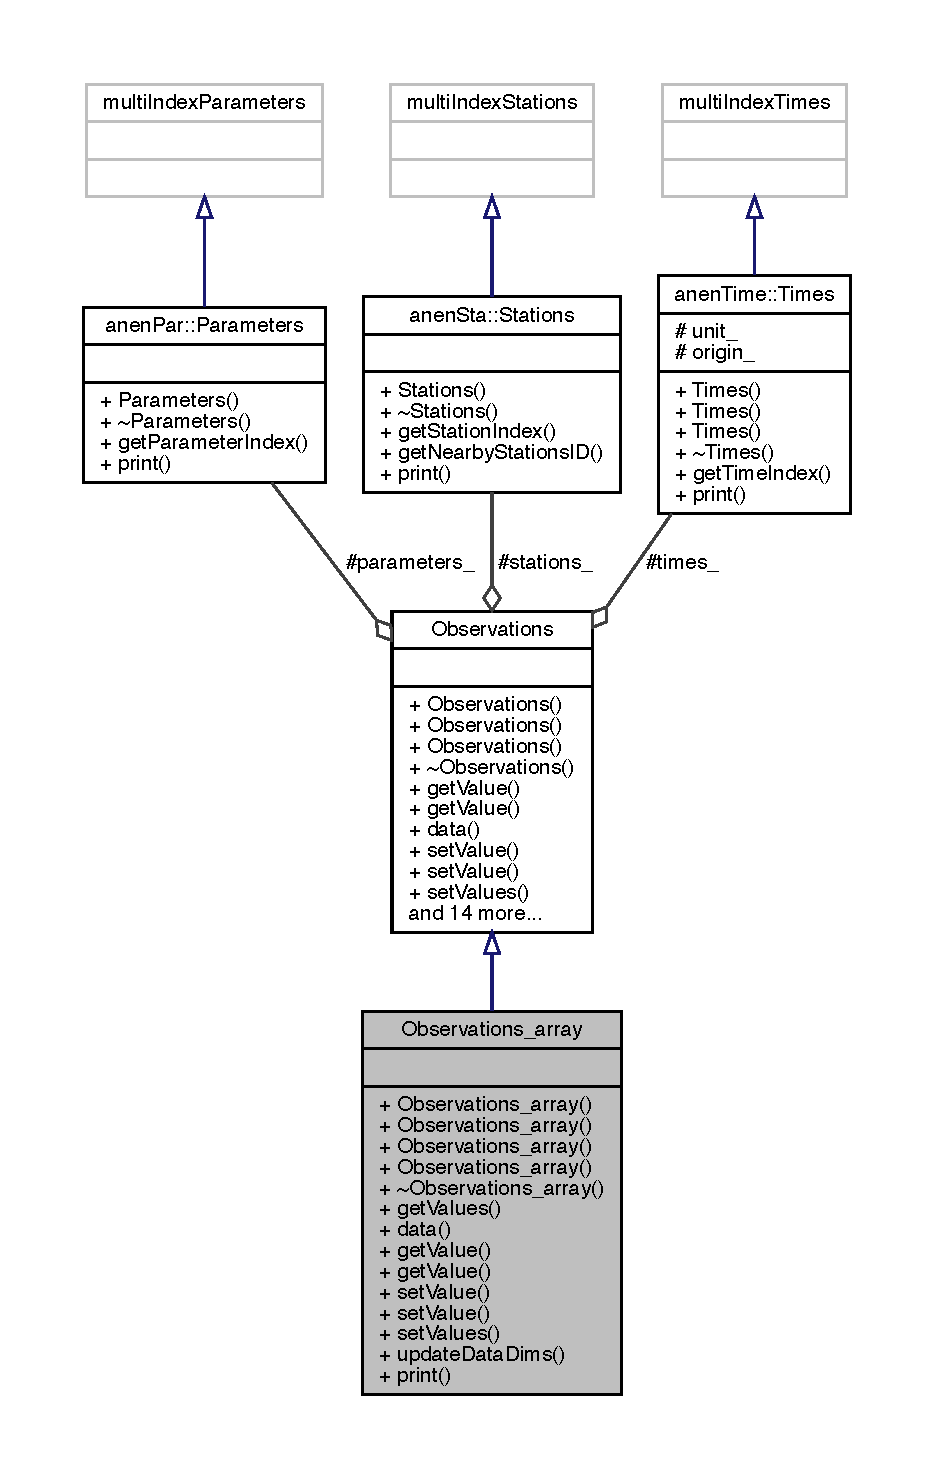
\includegraphics[height=550pt]{class_observations__array__coll__graph}
\end{center}
\end{figure}
\subsection*{Public Member Functions}
\begin{DoxyCompactItemize}
\item 
\mbox{\hyperlink{class_observations__array_a731dad95d0454c5848583a91e064a9cd}{Observations\+\_\+array}} ()=delete
\item 
\mbox{\hyperlink{class_observations__array_aa448781dd6c9c75fd3fa8ebf0e41e86d}{Observations\+\_\+array}} (const \mbox{\hyperlink{class_observations__array}{Observations\+\_\+array}} \&orig)=delete
\item 
\mbox{\hyperlink{class_observations__array_a33b9edf2cac9cfc23ba555c9362a2fc7}{Observations\+\_\+array}} (\mbox{\hyperlink{class_parameters}{Parameters}}, \mbox{\hyperlink{class_stations}{Stations}}, \mbox{\hyperlink{class_times}{Times}})
\item 
virtual \mbox{\hyperlink{class_observations__array_a3124448be571f561a2bd2e8b44c95a2e}{$\sim$\+Observations\+\_\+array}} ()
\item 
double \mbox{\hyperlink{class_observations__array_a33f2154b3fed9d488e06e8c92eecc4db}{get\+Value}} (std\+::size\+\_\+t parameter\+\_\+\+ID, std\+::size\+\_\+t station\+\_\+\+ID, double timestamp) const override
\item 
bool \mbox{\hyperlink{class_observations__array_a1708fe12a750cb68bb60782ab184605b}{set\+Value}} (double, std\+::size\+\_\+t parameter\+\_\+\+ID, std\+::size\+\_\+t station\+\_\+\+ID, double timestamp) override
\item 
bool \mbox{\hyperlink{class_observations__array_a59ee8d2a6b0d0158a3efa7c200c8ff43}{set\+Values}} (const std\+::vector$<$ double $>$ \&vals) override
\item 
void \mbox{\hyperlink{class_observations__array_a2563545e5a38ec7e3ec09380c0b38855}{print}} (std\+::ostream \&) const override
\end{DoxyCompactItemize}
\subsection*{Friends}
\begin{DoxyCompactItemize}
\item 
std\+::ostream \& \mbox{\hyperlink{class_observations__array_affb01c6a2af2ae2b833f7edec435234d}{operator$<$$<$}} (std\+::ostream \&, const \mbox{\hyperlink{class_observations__array}{Observations\+\_\+array}} \&)
\end{DoxyCompactItemize}
\subsection*{Additional Inherited Members}


\subsection{Constructor \& Destructor Documentation}
\mbox{\Hypertarget{class_observations__array_a731dad95d0454c5848583a91e064a9cd}\label{class_observations__array_a731dad95d0454c5848583a91e064a9cd}} 
\index{Observations\+\_\+array@{Observations\+\_\+array}!Observations\+\_\+array@{Observations\+\_\+array}}
\index{Observations\+\_\+array@{Observations\+\_\+array}!Observations\+\_\+array@{Observations\+\_\+array}}
\subsubsection{\texorpdfstring{Observations\+\_\+array()}{Observations\_array()}\hspace{0.1cm}{\footnotesize\ttfamily [1/3]}}
{\footnotesize\ttfamily Observations\+\_\+array\+::\+Observations\+\_\+array (\begin{DoxyParamCaption}{ }\end{DoxyParamCaption})\hspace{0.3cm}{\ttfamily [delete]}}

\mbox{\Hypertarget{class_observations__array_aa448781dd6c9c75fd3fa8ebf0e41e86d}\label{class_observations__array_aa448781dd6c9c75fd3fa8ebf0e41e86d}} 
\index{Observations\+\_\+array@{Observations\+\_\+array}!Observations\+\_\+array@{Observations\+\_\+array}}
\index{Observations\+\_\+array@{Observations\+\_\+array}!Observations\+\_\+array@{Observations\+\_\+array}}
\subsubsection{\texorpdfstring{Observations\+\_\+array()}{Observations\_array()}\hspace{0.1cm}{\footnotesize\ttfamily [2/3]}}
{\footnotesize\ttfamily Observations\+\_\+array\+::\+Observations\+\_\+array (\begin{DoxyParamCaption}\item[{const \mbox{\hyperlink{class_observations__array}{Observations\+\_\+array}} \&}]{orig }\end{DoxyParamCaption})\hspace{0.3cm}{\ttfamily [delete]}}

\mbox{\Hypertarget{class_observations__array_a33b9edf2cac9cfc23ba555c9362a2fc7}\label{class_observations__array_a33b9edf2cac9cfc23ba555c9362a2fc7}} 
\index{Observations\+\_\+array@{Observations\+\_\+array}!Observations\+\_\+array@{Observations\+\_\+array}}
\index{Observations\+\_\+array@{Observations\+\_\+array}!Observations\+\_\+array@{Observations\+\_\+array}}
\subsubsection{\texorpdfstring{Observations\+\_\+array()}{Observations\_array()}\hspace{0.1cm}{\footnotesize\ttfamily [3/3]}}
{\footnotesize\ttfamily Observations\+\_\+array\+::\+Observations\+\_\+array (\begin{DoxyParamCaption}\item[{\mbox{\hyperlink{class_parameters}{Parameters}}}]{parameters,  }\item[{\mbox{\hyperlink{class_stations}{Stations}}}]{stations,  }\item[{\mbox{\hyperlink{class_times}{Times}}}]{times }\end{DoxyParamCaption})}

\mbox{\Hypertarget{class_observations__array_a3124448be571f561a2bd2e8b44c95a2e}\label{class_observations__array_a3124448be571f561a2bd2e8b44c95a2e}} 
\index{Observations\+\_\+array@{Observations\+\_\+array}!````~Observations\+\_\+array@{$\sim$\+Observations\+\_\+array}}
\index{````~Observations\+\_\+array@{$\sim$\+Observations\+\_\+array}!Observations\+\_\+array@{Observations\+\_\+array}}
\subsubsection{\texorpdfstring{$\sim$\+Observations\+\_\+array()}{~Observations\_array()}}
{\footnotesize\ttfamily Observations\+\_\+array\+::$\sim$\+Observations\+\_\+array (\begin{DoxyParamCaption}{ }\end{DoxyParamCaption})\hspace{0.3cm}{\ttfamily [virtual]}}



\subsection{Member Function Documentation}
\mbox{\Hypertarget{class_observations__array_a33f2154b3fed9d488e06e8c92eecc4db}\label{class_observations__array_a33f2154b3fed9d488e06e8c92eecc4db}} 
\index{Observations\+\_\+array@{Observations\+\_\+array}!get\+Value@{get\+Value}}
\index{get\+Value@{get\+Value}!Observations\+\_\+array@{Observations\+\_\+array}}
\subsubsection{\texorpdfstring{get\+Value()}{getValue()}}
{\footnotesize\ttfamily double Observations\+\_\+array\+::get\+Value (\begin{DoxyParamCaption}\item[{std\+::size\+\_\+t}]{parameter\+\_\+\+ID,  }\item[{std\+::size\+\_\+t}]{station\+\_\+\+ID,  }\item[{double}]{timestamp }\end{DoxyParamCaption}) const\hspace{0.3cm}{\ttfamily [override]}, {\ttfamily [virtual]}}



Implements \mbox{\hyperlink{class_observations_ac5564bbf13e79d269407d1ecf567cd7f}{Observations}}.

\mbox{\Hypertarget{class_observations__array_a2563545e5a38ec7e3ec09380c0b38855}\label{class_observations__array_a2563545e5a38ec7e3ec09380c0b38855}} 
\index{Observations\+\_\+array@{Observations\+\_\+array}!print@{print}}
\index{print@{print}!Observations\+\_\+array@{Observations\+\_\+array}}
\subsubsection{\texorpdfstring{print()}{print()}}
{\footnotesize\ttfamily void Observations\+\_\+array\+::print (\begin{DoxyParamCaption}\item[{std\+::ostream \&}]{ }\end{DoxyParamCaption}) const\hspace{0.3cm}{\ttfamily [override]}, {\ttfamily [virtual]}}



Reimplemented from \mbox{\hyperlink{class_observations_a523647c5ae644959f0ed583cd7b11aba}{Observations}}.

\mbox{\Hypertarget{class_observations__array_a1708fe12a750cb68bb60782ab184605b}\label{class_observations__array_a1708fe12a750cb68bb60782ab184605b}} 
\index{Observations\+\_\+array@{Observations\+\_\+array}!set\+Value@{set\+Value}}
\index{set\+Value@{set\+Value}!Observations\+\_\+array@{Observations\+\_\+array}}
\subsubsection{\texorpdfstring{set\+Value()}{setValue()}}
{\footnotesize\ttfamily bool Observations\+\_\+array\+::set\+Value (\begin{DoxyParamCaption}\item[{double}]{,  }\item[{std\+::size\+\_\+t}]{parameter\+\_\+\+ID,  }\item[{std\+::size\+\_\+t}]{station\+\_\+\+ID,  }\item[{double}]{timestamp }\end{DoxyParamCaption})\hspace{0.3cm}{\ttfamily [override]}, {\ttfamily [virtual]}}



Implements \mbox{\hyperlink{class_observations_a359b5b8cd97cd43483444ca4fc188dff}{Observations}}.

\mbox{\Hypertarget{class_observations__array_a59ee8d2a6b0d0158a3efa7c200c8ff43}\label{class_observations__array_a59ee8d2a6b0d0158a3efa7c200c8ff43}} 
\index{Observations\+\_\+array@{Observations\+\_\+array}!set\+Values@{set\+Values}}
\index{set\+Values@{set\+Values}!Observations\+\_\+array@{Observations\+\_\+array}}
\subsubsection{\texorpdfstring{set\+Values()}{setValues()}}
{\footnotesize\ttfamily bool Observations\+\_\+array\+::set\+Values (\begin{DoxyParamCaption}\item[{const std\+::vector$<$ double $>$ \&}]{vals }\end{DoxyParamCaption})\hspace{0.3cm}{\ttfamily [override]}, {\ttfamily [virtual]}}

Sets data values from a vector.


\begin{DoxyParams}{Parameters}
{\em vals} & An std\+::vector$<$double$>$ object \\
\hline
\end{DoxyParams}
\begin{DoxyReturn}{Returns}
Returns true if succeed setting values. 
\end{DoxyReturn}


Implements \mbox{\hyperlink{class_observations_a58e9bcf10981845ad5bf89b34cacdbd7}{Observations}}.



\subsection{Friends And Related Function Documentation}
\mbox{\Hypertarget{class_observations__array_affb01c6a2af2ae2b833f7edec435234d}\label{class_observations__array_affb01c6a2af2ae2b833f7edec435234d}} 
\index{Observations\+\_\+array@{Observations\+\_\+array}!operator$<$$<$@{operator$<$$<$}}
\index{operator$<$$<$@{operator$<$$<$}!Observations\+\_\+array@{Observations\+\_\+array}}
\subsubsection{\texorpdfstring{operator$<$$<$}{operator<<}}
{\footnotesize\ttfamily std\+::ostream\& operator$<$$<$ (\begin{DoxyParamCaption}\item[{std\+::ostream \&}]{os,  }\item[{const \mbox{\hyperlink{class_observations__array}{Observations\+\_\+array}} \&}]{obj }\end{DoxyParamCaption})\hspace{0.3cm}{\ttfamily [friend]}}



The documentation for this class was generated from the following files\+:\begin{DoxyCompactItemize}
\item 
\mbox{\hyperlink{_observations_8h}{Observations.\+h}}\item 
\mbox{\hyperlink{_observations_8cpp}{Observations.\+cpp}}\end{DoxyCompactItemize}

\hypertarget{class_parameter}{}\section{Parameter Class Reference}
\label{class_parameter}\index{Parameter@{Parameter}}


Collaboration diagram for Parameter\+:
\nopagebreak
\begin{figure}[H]
\begin{center}
\leavevmode
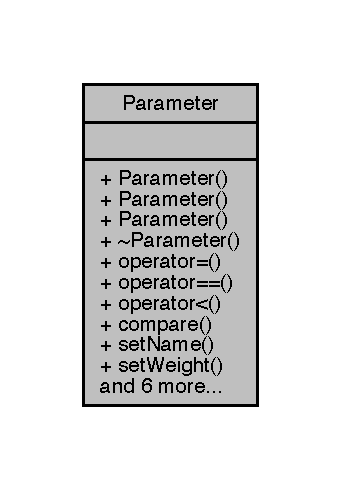
\includegraphics[width=143pt]{class_parameter__coll__graph}
\end{center}
\end{figure}


The documentation for this class was generated from the following file\+:\begin{DoxyCompactItemize}
\item 
\mbox{\hyperlink{_an_en_8cpp}{An\+En.\+cpp}}\end{DoxyCompactItemize}

\hypertarget{class_parameters}{}\section{Parameters Class Reference}
\label{class_parameters}\index{Parameters@{Parameters}}


Collaboration diagram for Parameters\+:
\nopagebreak
\begin{figure}[H]
\begin{center}
\leavevmode
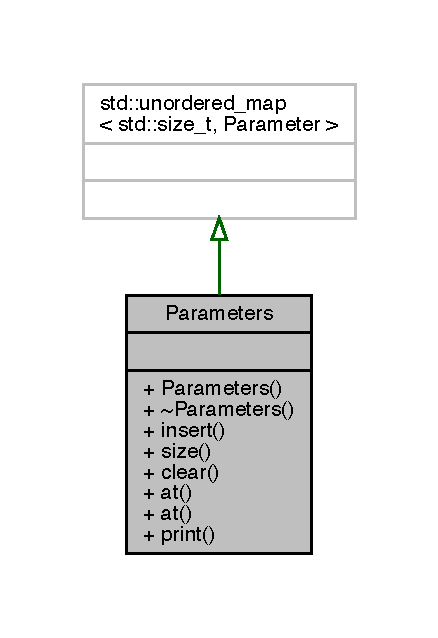
\includegraphics[width=148pt]{class_parameters__coll__graph}
\end{center}
\end{figure}


The documentation for this class was generated from the following file\+:\begin{DoxyCompactItemize}
\item 
\mbox{\hyperlink{_an_en_8cpp}{An\+En.\+cpp}}\end{DoxyCompactItemize}

\hypertarget{class_station}{}\section{Station Class Reference}
\label{class_station}\index{Station@{Station}}


{\ttfamily \#include $<$Stations.\+h$>$}



Collaboration diagram for Station\+:\nopagebreak
\begin{figure}[H]
\begin{center}
\leavevmode
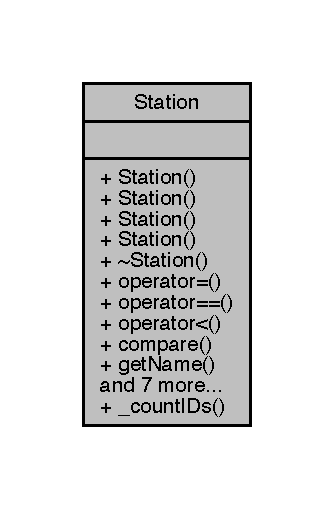
\includegraphics[width=160pt]{class_station__coll__graph}
\end{center}
\end{figure}
\subsection*{Public Member Functions}
\begin{DoxyCompactItemize}
\item 
\mbox{\hyperlink{class_station_a73d335726aad1d844d81cda6d9fd74e6}{Station}} ()
\item 
\mbox{\hyperlink{class_station_aeeba2cddaa328abff85cebfa5898b988}{Station}} (std\+::string)
\item 
\mbox{\hyperlink{class_station_a93320869206d6fdb35c6b314b03b9dd6}{Station}} (std\+::string, double, double)
\item 
\mbox{\hyperlink{class_station_aadb65bfb700ad2aee7dd4e7f62e40613}{Station}} (\mbox{\hyperlink{class_station}{Station}} const \&)
\item 
virtual \mbox{\hyperlink{class_station_a00434e79e8ee7f4ebd6d3b631dde5ac0}{$\sim$\+Station}} ()
\item 
\mbox{\hyperlink{class_station}{Station}} \& \mbox{\hyperlink{class_station_abaf887b87628c2bcd7e0af8626a4a1a4}{operator=}} (const \mbox{\hyperlink{class_station}{Station}} \&)
\item 
bool \mbox{\hyperlink{class_station_adae415f0267986c0056899ff4104cd5e}{operator==}} (const \mbox{\hyperlink{class_station}{Station}} \&) const
\item 
bool \mbox{\hyperlink{class_station_ad49b12012cb13c9f806587d9aa4c6fc9}{operator$<$}} (const \mbox{\hyperlink{class_station}{Station}} \&) const
\item 
bool \mbox{\hyperlink{class_station_a92f492a4766127e6ffbe993f0873708c}{compare}} (const \mbox{\hyperlink{class_station}{Station}} \&) const
\item 
std\+::string \mbox{\hyperlink{class_station_ac823ae175ec0e2baff462ed9612c7bae}{get\+Name}} () const
\item 
std\+::size\+\_\+t \mbox{\hyperlink{class_station_a69be6c90e4613e4166651ff6e67cfba2}{get\+ID}} () const
\item 
double \mbox{\hyperlink{class_station_aadddb2db193456d14bae16dbf2b8259f}{getY}} () const
\item 
double \mbox{\hyperlink{class_station_aa954dcd5d8f77ac9b91021b1e9c07735}{getX}} () const
\item 
void \mbox{\hyperlink{class_station_ad06d1756f0034a3f73ee1fe2993f87b9}{set\+Name}} (std\+::string name)
\item 
void \mbox{\hyperlink{class_station_ac9a83dadcfdcb36f477fed3c4586ff13}{setX}} (double x)
\item 
void \mbox{\hyperlink{class_station_a65a1d9f1121dc20515585594505e3a2e}{setY}} (double y)
\item 
void \mbox{\hyperlink{class_station_a1dfee264d3f636388b032675acb1302a}{print}} (std\+::ostream \&) const
\end{DoxyCompactItemize}
\subsection*{Static Public Member Functions}
\begin{DoxyCompactItemize}
\item 
static std\+::size\+\_\+t \mbox{\hyperlink{class_station_a0507e4875711fa10696ab05ec8cbc215}{\+\_\+count\+I\+Ds}} ()
\end{DoxyCompactItemize}
\subsection*{Friends}
\begin{DoxyCompactItemize}
\item 
std\+::ostream \& \mbox{\hyperlink{class_station_a98b2219804f7e593b080d3c8dec80f0b}{operator$<$$<$}} (std\+::ostream \&, \mbox{\hyperlink{class_station}{Station}} const \&)
\end{DoxyCompactItemize}


\subsection{Constructor \& Destructor Documentation}
\mbox{\Hypertarget{class_station_a73d335726aad1d844d81cda6d9fd74e6}\label{class_station_a73d335726aad1d844d81cda6d9fd74e6}} 
\index{Station@{Station}!Station@{Station}}
\index{Station@{Station}!Station@{Station}}
\subsubsection{\texorpdfstring{Station()}{Station()}\hspace{0.1cm}{\footnotesize\ttfamily [1/4]}}
{\footnotesize\ttfamily Station\+::\+Station (\begin{DoxyParamCaption}{ }\end{DoxyParamCaption})}

\mbox{\Hypertarget{class_station_aeeba2cddaa328abff85cebfa5898b988}\label{class_station_aeeba2cddaa328abff85cebfa5898b988}} 
\index{Station@{Station}!Station@{Station}}
\index{Station@{Station}!Station@{Station}}
\subsubsection{\texorpdfstring{Station()}{Station()}\hspace{0.1cm}{\footnotesize\ttfamily [2/4]}}
{\footnotesize\ttfamily Station\+::\+Station (\begin{DoxyParamCaption}\item[{std\+::string}]{name }\end{DoxyParamCaption})}

\mbox{\Hypertarget{class_station_a93320869206d6fdb35c6b314b03b9dd6}\label{class_station_a93320869206d6fdb35c6b314b03b9dd6}} 
\index{Station@{Station}!Station@{Station}}
\index{Station@{Station}!Station@{Station}}
\subsubsection{\texorpdfstring{Station()}{Station()}\hspace{0.1cm}{\footnotesize\ttfamily [3/4]}}
{\footnotesize\ttfamily Station\+::\+Station (\begin{DoxyParamCaption}\item[{std\+::string}]{,  }\item[{double}]{,  }\item[{double}]{ }\end{DoxyParamCaption})}

\mbox{\Hypertarget{class_station_aadb65bfb700ad2aee7dd4e7f62e40613}\label{class_station_aadb65bfb700ad2aee7dd4e7f62e40613}} 
\index{Station@{Station}!Station@{Station}}
\index{Station@{Station}!Station@{Station}}
\subsubsection{\texorpdfstring{Station()}{Station()}\hspace{0.1cm}{\footnotesize\ttfamily [4/4]}}
{\footnotesize\ttfamily Station\+::\+Station (\begin{DoxyParamCaption}\item[{\mbox{\hyperlink{class_station}{Station}} const \&}]{rhs }\end{DoxyParamCaption})}

\mbox{\Hypertarget{class_station_a00434e79e8ee7f4ebd6d3b631dde5ac0}\label{class_station_a00434e79e8ee7f4ebd6d3b631dde5ac0}} 
\index{Station@{Station}!````~Station@{$\sim$\+Station}}
\index{````~Station@{$\sim$\+Station}!Station@{Station}}
\subsubsection{\texorpdfstring{$\sim$\+Station()}{~Station()}}
{\footnotesize\ttfamily Station\+::$\sim$\+Station (\begin{DoxyParamCaption}{ }\end{DoxyParamCaption})\hspace{0.3cm}{\ttfamily [virtual]}}



\subsection{Member Function Documentation}
\mbox{\Hypertarget{class_station_a0507e4875711fa10696ab05ec8cbc215}\label{class_station_a0507e4875711fa10696ab05ec8cbc215}} 
\index{Station@{Station}!\+\_\+count\+I\+Ds@{\+\_\+count\+I\+Ds}}
\index{\+\_\+count\+I\+Ds@{\+\_\+count\+I\+Ds}!Station@{Station}}
\subsubsection{\texorpdfstring{\+\_\+count\+I\+Ds()}{\_countIDs()}}
{\footnotesize\ttfamily static std\+::size\+\_\+t Station\+::\+\_\+count\+I\+Ds (\begin{DoxyParamCaption}{ }\end{DoxyParamCaption})\hspace{0.3cm}{\ttfamily [inline]}, {\ttfamily [static]}}

\mbox{\Hypertarget{class_station_a92f492a4766127e6ffbe993f0873708c}\label{class_station_a92f492a4766127e6ffbe993f0873708c}} 
\index{Station@{Station}!compare@{compare}}
\index{compare@{compare}!Station@{Station}}
\subsubsection{\texorpdfstring{compare()}{compare()}}
{\footnotesize\ttfamily bool Station\+::compare (\begin{DoxyParamCaption}\item[{const \mbox{\hyperlink{class_station}{Station}} \&}]{rhs }\end{DoxyParamCaption}) const}

\mbox{\Hypertarget{class_station_a69be6c90e4613e4166651ff6e67cfba2}\label{class_station_a69be6c90e4613e4166651ff6e67cfba2}} 
\index{Station@{Station}!get\+ID@{get\+ID}}
\index{get\+ID@{get\+ID}!Station@{Station}}
\subsubsection{\texorpdfstring{get\+I\+D()}{getID()}}
{\footnotesize\ttfamily size\+\_\+t Station\+::get\+ID (\begin{DoxyParamCaption}{ }\end{DoxyParamCaption}) const}

\mbox{\Hypertarget{class_station_ac823ae175ec0e2baff462ed9612c7bae}\label{class_station_ac823ae175ec0e2baff462ed9612c7bae}} 
\index{Station@{Station}!get\+Name@{get\+Name}}
\index{get\+Name@{get\+Name}!Station@{Station}}
\subsubsection{\texorpdfstring{get\+Name()}{getName()}}
{\footnotesize\ttfamily string Station\+::get\+Name (\begin{DoxyParamCaption}{ }\end{DoxyParamCaption}) const}

\mbox{\Hypertarget{class_station_aa954dcd5d8f77ac9b91021b1e9c07735}\label{class_station_aa954dcd5d8f77ac9b91021b1e9c07735}} 
\index{Station@{Station}!getX@{getX}}
\index{getX@{getX}!Station@{Station}}
\subsubsection{\texorpdfstring{get\+X()}{getX()}}
{\footnotesize\ttfamily double Station\+::getX (\begin{DoxyParamCaption}{ }\end{DoxyParamCaption}) const}

\mbox{\Hypertarget{class_station_aadddb2db193456d14bae16dbf2b8259f}\label{class_station_aadddb2db193456d14bae16dbf2b8259f}} 
\index{Station@{Station}!getY@{getY}}
\index{getY@{getY}!Station@{Station}}
\subsubsection{\texorpdfstring{get\+Y()}{getY()}}
{\footnotesize\ttfamily double Station\+::getY (\begin{DoxyParamCaption}{ }\end{DoxyParamCaption}) const}

\mbox{\Hypertarget{class_station_ad49b12012cb13c9f806587d9aa4c6fc9}\label{class_station_ad49b12012cb13c9f806587d9aa4c6fc9}} 
\index{Station@{Station}!operator$<$@{operator$<$}}
\index{operator$<$@{operator$<$}!Station@{Station}}
\subsubsection{\texorpdfstring{operator$<$()}{operator<()}}
{\footnotesize\ttfamily bool Station\+::operator$<$ (\begin{DoxyParamCaption}\item[{const \mbox{\hyperlink{class_station}{Station}} \&}]{rhs }\end{DoxyParamCaption}) const}

\mbox{\Hypertarget{class_station_abaf887b87628c2bcd7e0af8626a4a1a4}\label{class_station_abaf887b87628c2bcd7e0af8626a4a1a4}} 
\index{Station@{Station}!operator=@{operator=}}
\index{operator=@{operator=}!Station@{Station}}
\subsubsection{\texorpdfstring{operator=()}{operator=()}}
{\footnotesize\ttfamily \mbox{\hyperlink{class_station}{Station}} \& Station\+::operator= (\begin{DoxyParamCaption}\item[{const \mbox{\hyperlink{class_station}{Station}} \&}]{rhs }\end{DoxyParamCaption})}

\mbox{\Hypertarget{class_station_adae415f0267986c0056899ff4104cd5e}\label{class_station_adae415f0267986c0056899ff4104cd5e}} 
\index{Station@{Station}!operator==@{operator==}}
\index{operator==@{operator==}!Station@{Station}}
\subsubsection{\texorpdfstring{operator==()}{operator==()}}
{\footnotesize\ttfamily bool Station\+::operator== (\begin{DoxyParamCaption}\item[{const \mbox{\hyperlink{class_station}{Station}} \&}]{rhs }\end{DoxyParamCaption}) const}

\mbox{\Hypertarget{class_station_a1dfee264d3f636388b032675acb1302a}\label{class_station_a1dfee264d3f636388b032675acb1302a}} 
\index{Station@{Station}!print@{print}}
\index{print@{print}!Station@{Station}}
\subsubsection{\texorpdfstring{print()}{print()}}
{\footnotesize\ttfamily void Station\+::print (\begin{DoxyParamCaption}\item[{std\+::ostream \&}]{ }\end{DoxyParamCaption}) const}

\mbox{\Hypertarget{class_station_ad06d1756f0034a3f73ee1fe2993f87b9}\label{class_station_ad06d1756f0034a3f73ee1fe2993f87b9}} 
\index{Station@{Station}!set\+Name@{set\+Name}}
\index{set\+Name@{set\+Name}!Station@{Station}}
\subsubsection{\texorpdfstring{set\+Name()}{setName()}}
{\footnotesize\ttfamily void Station\+::set\+Name (\begin{DoxyParamCaption}\item[{std\+::string}]{name }\end{DoxyParamCaption})}

\mbox{\Hypertarget{class_station_ac9a83dadcfdcb36f477fed3c4586ff13}\label{class_station_ac9a83dadcfdcb36f477fed3c4586ff13}} 
\index{Station@{Station}!setX@{setX}}
\index{setX@{setX}!Station@{Station}}
\subsubsection{\texorpdfstring{set\+X()}{setX()}}
{\footnotesize\ttfamily void Station\+::setX (\begin{DoxyParamCaption}\item[{double}]{x }\end{DoxyParamCaption})}

\mbox{\Hypertarget{class_station_a65a1d9f1121dc20515585594505e3a2e}\label{class_station_a65a1d9f1121dc20515585594505e3a2e}} 
\index{Station@{Station}!setY@{setY}}
\index{setY@{setY}!Station@{Station}}
\subsubsection{\texorpdfstring{set\+Y()}{setY()}}
{\footnotesize\ttfamily void Station\+::setY (\begin{DoxyParamCaption}\item[{double}]{y }\end{DoxyParamCaption})}



\subsection{Friends And Related Function Documentation}
\mbox{\Hypertarget{class_station_a98b2219804f7e593b080d3c8dec80f0b}\label{class_station_a98b2219804f7e593b080d3c8dec80f0b}} 
\index{Station@{Station}!operator$<$$<$@{operator$<$$<$}}
\index{operator$<$$<$@{operator$<$$<$}!Station@{Station}}
\subsubsection{\texorpdfstring{operator$<$$<$}{operator<<}}
{\footnotesize\ttfamily std\+::ostream\& operator$<$$<$ (\begin{DoxyParamCaption}\item[{std\+::ostream \&}]{,  }\item[{\mbox{\hyperlink{class_station}{Station}} const \&}]{ }\end{DoxyParamCaption})\hspace{0.3cm}{\ttfamily [friend]}}



The documentation for this class was generated from the following files\+:\begin{DoxyCompactItemize}
\item 
\mbox{\hyperlink{_stations_8h}{Stations.\+h}}\item 
\mbox{\hyperlink{_stations_8cpp}{Stations.\+cpp}}\end{DoxyCompactItemize}

\hypertarget{class_stations}{}\section{Stations Class Reference}
\label{class_stations}\index{Stations@{Stations}}


{\ttfamily \#include $<$Stations.\+h$>$}



Inheritance diagram for Stations\+:
\nopagebreak
\begin{figure}[H]
\begin{center}
\leavevmode
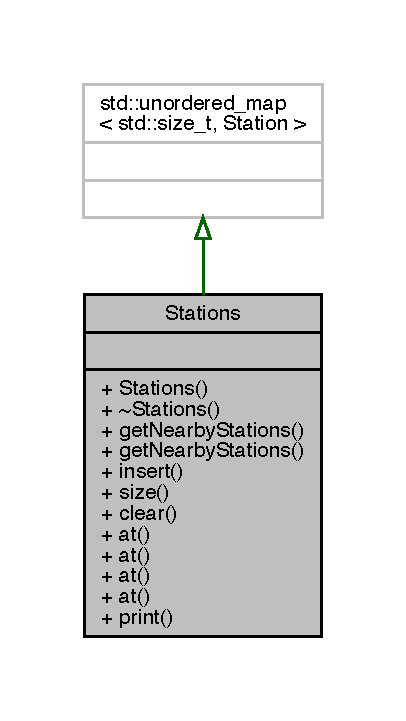
\includegraphics[width=195pt]{class_stations__inherit__graph}
\end{center}
\end{figure}


Collaboration diagram for Stations\+:
\nopagebreak
\begin{figure}[H]
\begin{center}
\leavevmode
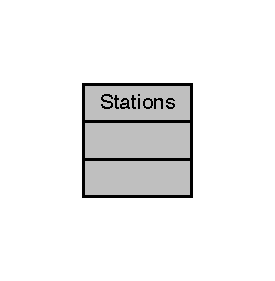
\includegraphics[width=195pt]{class_stations__coll__graph}
\end{center}
\end{figure}
\subsection*{Public Member Functions}
\begin{DoxyCompactItemize}
\item 
\mbox{\hyperlink{class_stations_a4e0f8fc4709bd680154b7be896ca2350}{Stations}} ()
\item 
virtual \mbox{\hyperlink{class_stations_a9d17c76f77babd7e88adf95112825b1d}{$\sim$\+Stations}} ()
\item 
std\+::vector$<$ std\+::size\+\_\+t $>$ \mbox{\hyperlink{class_stations_ac0438c6c8639d209dfc3937cfd993723}{get\+Nearby\+Stations}} (const \mbox{\hyperlink{class_station}{Station}} \&) const
\item 
std\+::vector$<$ std\+::size\+\_\+t $>$ \mbox{\hyperlink{class_stations_afebcca23df46c02b2d4dfe53da2f03d1}{get\+Nearby\+Stations}} (const std\+::size\+\_\+t \&) const
\item 
std\+::pair$<$ iterator, bool $>$ \mbox{\hyperlink{class_stations_abe1318af7b69c4eb586b099af6a1f6b8}{insert}} (const \mbox{\hyperlink{class_station}{Station}} \&station)
\item 
size\+\_\+t \mbox{\hyperlink{class_stations_ab6e3d3635fffe60f813b1fa7c28e4d8c}{size}} () const \+\_\+\+N\+O\+E\+X\+C\+E\+PT
\item 
void \mbox{\hyperlink{class_stations_ae75fd812e17138fec710fd1e75032239}{clear}} () \+\_\+\+N\+O\+E\+X\+C\+E\+PT
\item 
\mbox{\hyperlink{class_station}{Station}} \& \mbox{\hyperlink{class_stations_a1d2abb378db9aa8deb9f7b54aefac2dd}{at}} (const size\+\_\+t \&key)
\item 
\mbox{\hyperlink{class_station}{Station}} \& \mbox{\hyperlink{class_stations_a0db00fc62fdeebde93f2624477074087}{at}} (const \mbox{\hyperlink{class_station}{Station}} \&station)
\item 
const \mbox{\hyperlink{class_station}{Station}} \& \mbox{\hyperlink{class_stations_ab785e4995153a682ac3fd739b99e8db3}{at}} (const size\+\_\+t \&key) const
\item 
const \mbox{\hyperlink{class_station}{Station}} \& \mbox{\hyperlink{class_stations_a76175b88bafb7de42fae0a5d7518aac9}{at}} (const \mbox{\hyperlink{class_station}{Station}} \&station) const
\item 
void \mbox{\hyperlink{class_stations_ae62b158dedf5f15c385671d15b950dc5}{print}} (std\+::ostream \&) const
\end{DoxyCompactItemize}
\subsection*{Friends}
\begin{DoxyCompactItemize}
\item 
std\+::ostream \& \mbox{\hyperlink{class_stations_a6c2ba44849c083fa6d206d4573ea523e}{operator$<$$<$}} (std\+::ostream \&, \mbox{\hyperlink{class_stations}{Stations}} const \&)
\end{DoxyCompactItemize}


\subsection{Detailed Description}
\mbox{\hyperlink{class_stations}{Stations}} is a protected inheritance from std\+::unordered\+\_\+map$<$std\+::size\+\_\+t, Station$>$ because certain functions, like the insert function, have different behaviors. 

\subsection{Constructor \& Destructor Documentation}
\mbox{\Hypertarget{class_stations_a4e0f8fc4709bd680154b7be896ca2350}\label{class_stations_a4e0f8fc4709bd680154b7be896ca2350}} 
\index{Stations@{Stations}!Stations@{Stations}}
\index{Stations@{Stations}!Stations@{Stations}}
\subsubsection{\texorpdfstring{Stations()}{Stations()}}
{\footnotesize\ttfamily Stations\+::\+Stations (\begin{DoxyParamCaption}{ }\end{DoxyParamCaption})}

\mbox{\Hypertarget{class_stations_a9d17c76f77babd7e88adf95112825b1d}\label{class_stations_a9d17c76f77babd7e88adf95112825b1d}} 
\index{Stations@{Stations}!````~Stations@{$\sim$\+Stations}}
\index{````~Stations@{$\sim$\+Stations}!Stations@{Stations}}
\subsubsection{\texorpdfstring{$\sim$\+Stations()}{~Stations()}}
{\footnotesize\ttfamily Stations\+::$\sim$\+Stations (\begin{DoxyParamCaption}{ }\end{DoxyParamCaption})\hspace{0.3cm}{\ttfamily [virtual]}}



\subsection{Member Function Documentation}
\mbox{\Hypertarget{class_stations_a1d2abb378db9aa8deb9f7b54aefac2dd}\label{class_stations_a1d2abb378db9aa8deb9f7b54aefac2dd}} 
\index{Stations@{Stations}!at@{at}}
\index{at@{at}!Stations@{Stations}}
\subsubsection{\texorpdfstring{at()}{at()}\hspace{0.1cm}{\footnotesize\ttfamily [1/4]}}
{\footnotesize\ttfamily \mbox{\hyperlink{class_station}{Station}} \& Stations\+::at (\begin{DoxyParamCaption}\item[{const size\+\_\+t \&}]{key }\end{DoxyParamCaption})}

Gets the reference to the \mbox{\hyperlink{class_station}{Station}} based on the ID. If no such element exists, an exception of type std\+::out\+\_\+of\+\_\+range is thrown.


\begin{DoxyParams}{Parameters}
{\em key} & An size\+\_\+t key. \\
\hline
\end{DoxyParams}
\begin{DoxyReturn}{Returns}
A reference to \mbox{\hyperlink{class_station}{Station}} object. 
\end{DoxyReturn}
\mbox{\Hypertarget{class_stations_a0db00fc62fdeebde93f2624477074087}\label{class_stations_a0db00fc62fdeebde93f2624477074087}} 
\index{Stations@{Stations}!at@{at}}
\index{at@{at}!Stations@{Stations}}
\subsubsection{\texorpdfstring{at()}{at()}\hspace{0.1cm}{\footnotesize\ttfamily [2/4]}}
{\footnotesize\ttfamily \mbox{\hyperlink{class_station}{Station}} \& Stations\+::at (\begin{DoxyParamCaption}\item[{const \mbox{\hyperlink{class_station}{Station}} \&}]{station }\end{DoxyParamCaption})}

\mbox{\Hypertarget{class_stations_ab785e4995153a682ac3fd739b99e8db3}\label{class_stations_ab785e4995153a682ac3fd739b99e8db3}} 
\index{Stations@{Stations}!at@{at}}
\index{at@{at}!Stations@{Stations}}
\subsubsection{\texorpdfstring{at()}{at()}\hspace{0.1cm}{\footnotesize\ttfamily [3/4]}}
{\footnotesize\ttfamily const \mbox{\hyperlink{class_station}{Station}} \& Stations\+::at (\begin{DoxyParamCaption}\item[{const size\+\_\+t \&}]{key }\end{DoxyParamCaption}) const}

\mbox{\Hypertarget{class_stations_a76175b88bafb7de42fae0a5d7518aac9}\label{class_stations_a76175b88bafb7de42fae0a5d7518aac9}} 
\index{Stations@{Stations}!at@{at}}
\index{at@{at}!Stations@{Stations}}
\subsubsection{\texorpdfstring{at()}{at()}\hspace{0.1cm}{\footnotesize\ttfamily [4/4]}}
{\footnotesize\ttfamily const \mbox{\hyperlink{class_station}{Station}} \& Stations\+::at (\begin{DoxyParamCaption}\item[{const \mbox{\hyperlink{class_station}{Station}} \&}]{station }\end{DoxyParamCaption}) const}

\mbox{\Hypertarget{class_stations_ae75fd812e17138fec710fd1e75032239}\label{class_stations_ae75fd812e17138fec710fd1e75032239}} 
\index{Stations@{Stations}!clear@{clear}}
\index{clear@{clear}!Stations@{Stations}}
\subsubsection{\texorpdfstring{clear()}{clear()}}
{\footnotesize\ttfamily void Stations\+::clear (\begin{DoxyParamCaption}{ }\end{DoxyParamCaption})}

\mbox{\Hypertarget{class_stations_ac0438c6c8639d209dfc3937cfd993723}\label{class_stations_ac0438c6c8639d209dfc3937cfd993723}} 
\index{Stations@{Stations}!get\+Nearby\+Stations@{get\+Nearby\+Stations}}
\index{get\+Nearby\+Stations@{get\+Nearby\+Stations}!Stations@{Stations}}
\subsubsection{\texorpdfstring{get\+Nearby\+Stations()}{getNearbyStations()}\hspace{0.1cm}{\footnotesize\ttfamily [1/2]}}
{\footnotesize\ttfamily vector$<$ size\+\_\+t $>$ Stations\+::get\+Nearby\+Stations (\begin{DoxyParamCaption}\item[{const \mbox{\hyperlink{class_station}{Station}} \&}]{station }\end{DoxyParamCaption}) const}

\mbox{\Hypertarget{class_stations_afebcca23df46c02b2d4dfe53da2f03d1}\label{class_stations_afebcca23df46c02b2d4dfe53da2f03d1}} 
\index{Stations@{Stations}!get\+Nearby\+Stations@{get\+Nearby\+Stations}}
\index{get\+Nearby\+Stations@{get\+Nearby\+Stations}!Stations@{Stations}}
\subsubsection{\texorpdfstring{get\+Nearby\+Stations()}{getNearbyStations()}\hspace{0.1cm}{\footnotesize\ttfamily [2/2]}}
{\footnotesize\ttfamily std\+::vector$<$std\+::size\+\_\+t$>$ Stations\+::get\+Nearby\+Stations (\begin{DoxyParamCaption}\item[{const std\+::size\+\_\+t \&}]{ }\end{DoxyParamCaption}) const}

\mbox{\Hypertarget{class_stations_abe1318af7b69c4eb586b099af6a1f6b8}\label{class_stations_abe1318af7b69c4eb586b099af6a1f6b8}} 
\index{Stations@{Stations}!insert@{insert}}
\index{insert@{insert}!Stations@{Stations}}
\subsubsection{\texorpdfstring{insert()}{insert()}}
{\footnotesize\ttfamily std\+::pair$<$iterator, bool$>$ Stations\+::insert (\begin{DoxyParamCaption}\item[{const \mbox{\hyperlink{class_station}{Station}} \&}]{station }\end{DoxyParamCaption})\hspace{0.3cm}{\ttfamily [inline]}}

Inserts a station into the map with the key set to its ID. By this way, it is ensured that stations are unique in the map with their ID as the key.


\begin{DoxyParams}{Parameters}
{\em station} & \mbox{\hyperlink{class_station}{Station}} object. \\
\hline
\end{DoxyParams}
\begin{DoxyReturn}{Returns}
std\+::pair$<$iterator, bool$>$ object consisting of an iterator to the inserted element (or to the element that prevented the insertion) and a bool denoting whether the insertion took place. 
\end{DoxyReturn}
\mbox{\Hypertarget{class_stations_ae62b158dedf5f15c385671d15b950dc5}\label{class_stations_ae62b158dedf5f15c385671d15b950dc5}} 
\index{Stations@{Stations}!print@{print}}
\index{print@{print}!Stations@{Stations}}
\subsubsection{\texorpdfstring{print()}{print()}}
{\footnotesize\ttfamily void Stations\+::print (\begin{DoxyParamCaption}\item[{std\+::ostream \&}]{ }\end{DoxyParamCaption}) const}

\mbox{\Hypertarget{class_stations_ab6e3d3635fffe60f813b1fa7c28e4d8c}\label{class_stations_ab6e3d3635fffe60f813b1fa7c28e4d8c}} 
\index{Stations@{Stations}!size@{size}}
\index{size@{size}!Stations@{Stations}}
\subsubsection{\texorpdfstring{size()}{size()}}
{\footnotesize\ttfamily size\+\_\+t Stations\+::size (\begin{DoxyParamCaption}{ }\end{DoxyParamCaption}) const}



\subsection{Friends And Related Function Documentation}
\mbox{\Hypertarget{class_stations_a6c2ba44849c083fa6d206d4573ea523e}\label{class_stations_a6c2ba44849c083fa6d206d4573ea523e}} 
\index{Stations@{Stations}!operator$<$$<$@{operator$<$$<$}}
\index{operator$<$$<$@{operator$<$$<$}!Stations@{Stations}}
\subsubsection{\texorpdfstring{operator$<$$<$}{operator<<}}
{\footnotesize\ttfamily std\+::ostream\& operator$<$$<$ (\begin{DoxyParamCaption}\item[{std\+::ostream \&}]{,  }\item[{\mbox{\hyperlink{class_stations}{Stations}} const \&}]{ }\end{DoxyParamCaption})\hspace{0.3cm}{\ttfamily [friend]}}



The documentation for this class was generated from the following files\+:\begin{DoxyCompactItemize}
\item 
\mbox{\hyperlink{_stations_8h}{Stations.\+h}}\item 
\mbox{\hyperlink{_stations_8cpp}{Stations.\+cpp}}\end{DoxyCompactItemize}

\hypertarget{class_times}{}\section{Times Class Reference}
\label{class_times}\index{Times@{Times}}


\mbox{\hyperlink{class_times}{Times}} class is used to store time information for predictions.  




{\ttfamily \#include $<$Times.\+h$>$}



Inheritance diagram for Times\+:
\nopagebreak
\begin{figure}[H]
\begin{center}
\leavevmode
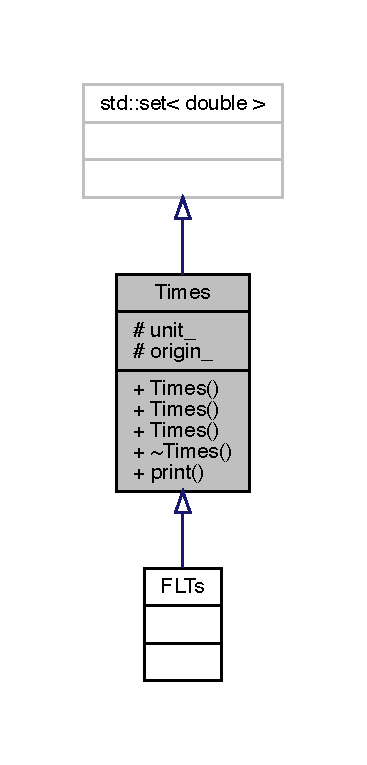
\includegraphics[width=176pt]{class_times__inherit__graph}
\end{center}
\end{figure}


Collaboration diagram for Times\+:\nopagebreak
\begin{figure}[H]
\begin{center}
\leavevmode
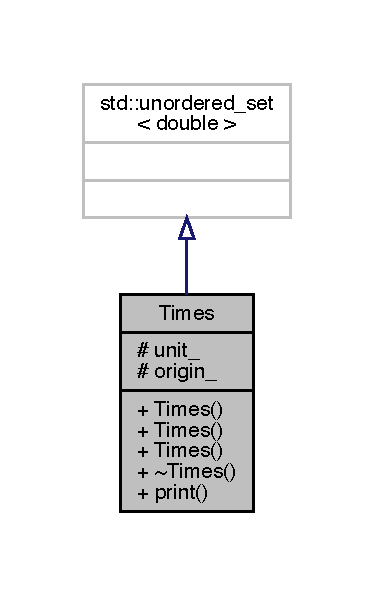
\includegraphics[width=176pt]{class_times__coll__graph}
\end{center}
\end{figure}
\subsection*{Public Member Functions}
\begin{DoxyCompactItemize}
\item 
\mbox{\hyperlink{class_times_a8ba246100f3c12f80abeb3beb93446f6}{Times}} ()
\item 
\mbox{\hyperlink{class_times_a49de9639125c133a6b0e4351eaa422b5}{Times}} (std\+::string unit)
\item 
\mbox{\hyperlink{class_times_aec85fed5d7741b4ea2445874b3ecadfe}{Times}} (std\+::string unit, std\+::string origin)
\item 
virtual \mbox{\hyperlink{class_times_a7989831a284e9d10e3ae96ceb2349a3c}{$\sim$\+Times}} ()
\item 
void \mbox{\hyperlink{class_times_acdfa95279c544d2cee2f33415fe4909c}{print}} (std\+::ostream \&os) const
\end{DoxyCompactItemize}
\subsection*{Protected Attributes}
\begin{DoxyCompactItemize}
\item 
std\+::string \mbox{\hyperlink{class_times_a32130156e076d5511c44fc71ee68a980}{unit\+\_\+}} = \char`\"{}seconds\char`\"{}
\item 
std\+::string \mbox{\hyperlink{class_times_a7609195d9216105cad01df13230abfa9}{origin\+\_\+}}
\end{DoxyCompactItemize}
\subsection*{Friends}
\begin{DoxyCompactItemize}
\item 
std\+::ostream \& \mbox{\hyperlink{class_times_a0c37c7d9833e9b02d1a219555f55fe34}{operator$<$$<$}} (std\+::ostream \&os, \mbox{\hyperlink{class_times}{Times}} const \&obj)
\end{DoxyCompactItemize}


\subsection{Detailed Description}
\mbox{\hyperlink{class_times}{Times}} class is used to store time information for predictions. 

\mbox{\hyperlink{class_times}{Times}} class supports the following features\+:
\begin{DoxyEnumerate}
\item Timestamps are unique in \mbox{\hyperlink{class_times}{Times}};
\item Timestamps are kept in sequence of insertion, and accessible through random access; 
\end{DoxyEnumerate}

\subsection{Constructor \& Destructor Documentation}
\mbox{\Hypertarget{class_times_a8ba246100f3c12f80abeb3beb93446f6}\label{class_times_a8ba246100f3c12f80abeb3beb93446f6}} 
\index{Times@{Times}!Times@{Times}}
\index{Times@{Times}!Times@{Times}}
\subsubsection{\texorpdfstring{Times()}{Times()}\hspace{0.1cm}{\footnotesize\ttfamily [1/3]}}
{\footnotesize\ttfamily Times\+::\+Times (\begin{DoxyParamCaption}{ }\end{DoxyParamCaption})}

\mbox{\Hypertarget{class_times_a49de9639125c133a6b0e4351eaa422b5}\label{class_times_a49de9639125c133a6b0e4351eaa422b5}} 
\index{Times@{Times}!Times@{Times}}
\index{Times@{Times}!Times@{Times}}
\subsubsection{\texorpdfstring{Times()}{Times()}\hspace{0.1cm}{\footnotesize\ttfamily [2/3]}}
{\footnotesize\ttfamily Times\+::\+Times (\begin{DoxyParamCaption}\item[{std\+::string}]{unit }\end{DoxyParamCaption})}

\mbox{\Hypertarget{class_times_aec85fed5d7741b4ea2445874b3ecadfe}\label{class_times_aec85fed5d7741b4ea2445874b3ecadfe}} 
\index{Times@{Times}!Times@{Times}}
\index{Times@{Times}!Times@{Times}}
\subsubsection{\texorpdfstring{Times()}{Times()}\hspace{0.1cm}{\footnotesize\ttfamily [3/3]}}
{\footnotesize\ttfamily Times\+::\+Times (\begin{DoxyParamCaption}\item[{std\+::string}]{unit,  }\item[{std\+::string}]{origin }\end{DoxyParamCaption})}

\mbox{\Hypertarget{class_times_a7989831a284e9d10e3ae96ceb2349a3c}\label{class_times_a7989831a284e9d10e3ae96ceb2349a3c}} 
\index{Times@{Times}!````~Times@{$\sim$\+Times}}
\index{````~Times@{$\sim$\+Times}!Times@{Times}}
\subsubsection{\texorpdfstring{$\sim$\+Times()}{~Times()}}
{\footnotesize\ttfamily Times\+::$\sim$\+Times (\begin{DoxyParamCaption}{ }\end{DoxyParamCaption})\hspace{0.3cm}{\ttfamily [virtual]}}



\subsection{Member Function Documentation}
\mbox{\Hypertarget{class_times_acdfa95279c544d2cee2f33415fe4909c}\label{class_times_acdfa95279c544d2cee2f33415fe4909c}} 
\index{Times@{Times}!print@{print}}
\index{print@{print}!Times@{Times}}
\subsubsection{\texorpdfstring{print()}{print()}}
{\footnotesize\ttfamily void Times\+::print (\begin{DoxyParamCaption}\item[{std\+::ostream \&}]{os }\end{DoxyParamCaption}) const}



\subsection{Friends And Related Function Documentation}
\mbox{\Hypertarget{class_times_a0c37c7d9833e9b02d1a219555f55fe34}\label{class_times_a0c37c7d9833e9b02d1a219555f55fe34}} 
\index{Times@{Times}!operator$<$$<$@{operator$<$$<$}}
\index{operator$<$$<$@{operator$<$$<$}!Times@{Times}}
\subsubsection{\texorpdfstring{operator$<$$<$}{operator<<}}
{\footnotesize\ttfamily std\+::ostream\& operator$<$$<$ (\begin{DoxyParamCaption}\item[{std\+::ostream \&}]{os,  }\item[{\mbox{\hyperlink{class_times}{Times}} const \&}]{obj }\end{DoxyParamCaption})\hspace{0.3cm}{\ttfamily [friend]}}



\subsection{Member Data Documentation}
\mbox{\Hypertarget{class_times_a7609195d9216105cad01df13230abfa9}\label{class_times_a7609195d9216105cad01df13230abfa9}} 
\index{Times@{Times}!origin\+\_\+@{origin\+\_\+}}
\index{origin\+\_\+@{origin\+\_\+}!Times@{Times}}
\subsubsection{\texorpdfstring{origin\+\_\+}{origin\_}}
{\footnotesize\ttfamily std\+::string Times\+::origin\+\_\+\hspace{0.3cm}{\ttfamily [protected]}}

\mbox{\Hypertarget{class_times_a32130156e076d5511c44fc71ee68a980}\label{class_times_a32130156e076d5511c44fc71ee68a980}} 
\index{Times@{Times}!unit\+\_\+@{unit\+\_\+}}
\index{unit\+\_\+@{unit\+\_\+}!Times@{Times}}
\subsubsection{\texorpdfstring{unit\+\_\+}{unit\_}}
{\footnotesize\ttfamily std\+::string Times\+::unit\+\_\+ = \char`\"{}seconds\char`\"{}\hspace{0.3cm}{\ttfamily [protected]}}



The documentation for this class was generated from the following files\+:\begin{DoxyCompactItemize}
\item 
\mbox{\hyperlink{_times_8h}{Times.\+h}}\item 
\mbox{\hyperlink{_times_8cpp}{Times.\+cpp}}\end{DoxyCompactItemize}

\chapter{File Documentation}
\hypertarget{_8dep_8inc}{}\section{.dep.\+inc File Reference}
\label{_8dep_8inc}\index{.\+dep.\+inc@{.\+dep.\+inc}}

\hypertarget{_an_en_i_o_8cpp}{}\section{An\+En\+I\+O.\+cpp File Reference}
\label{_an_en_i_o_8cpp}\index{An\+En\+I\+O.\+cpp@{An\+En\+I\+O.\+cpp}}
{\ttfamily \#include \char`\"{}An\+En\+I\+O.\+h\char`\"{}}\newline
{\ttfamily \#include $<$boost/filesystem.\+hpp$>$}\newline
{\ttfamily \#include $<$algorithm$>$}\newline
{\ttfamily \#include $<$exception$>$}\newline
{\ttfamily \#include $<$sstream$>$}\newline
{\ttfamily \#include $<$set$>$}\newline
{\ttfamily \#include $<$map$>$}\newline
Include dependency graph for An\+En\+I\+O.\+cpp\+:
\nopagebreak
\begin{figure}[H]
\begin{center}
\leavevmode
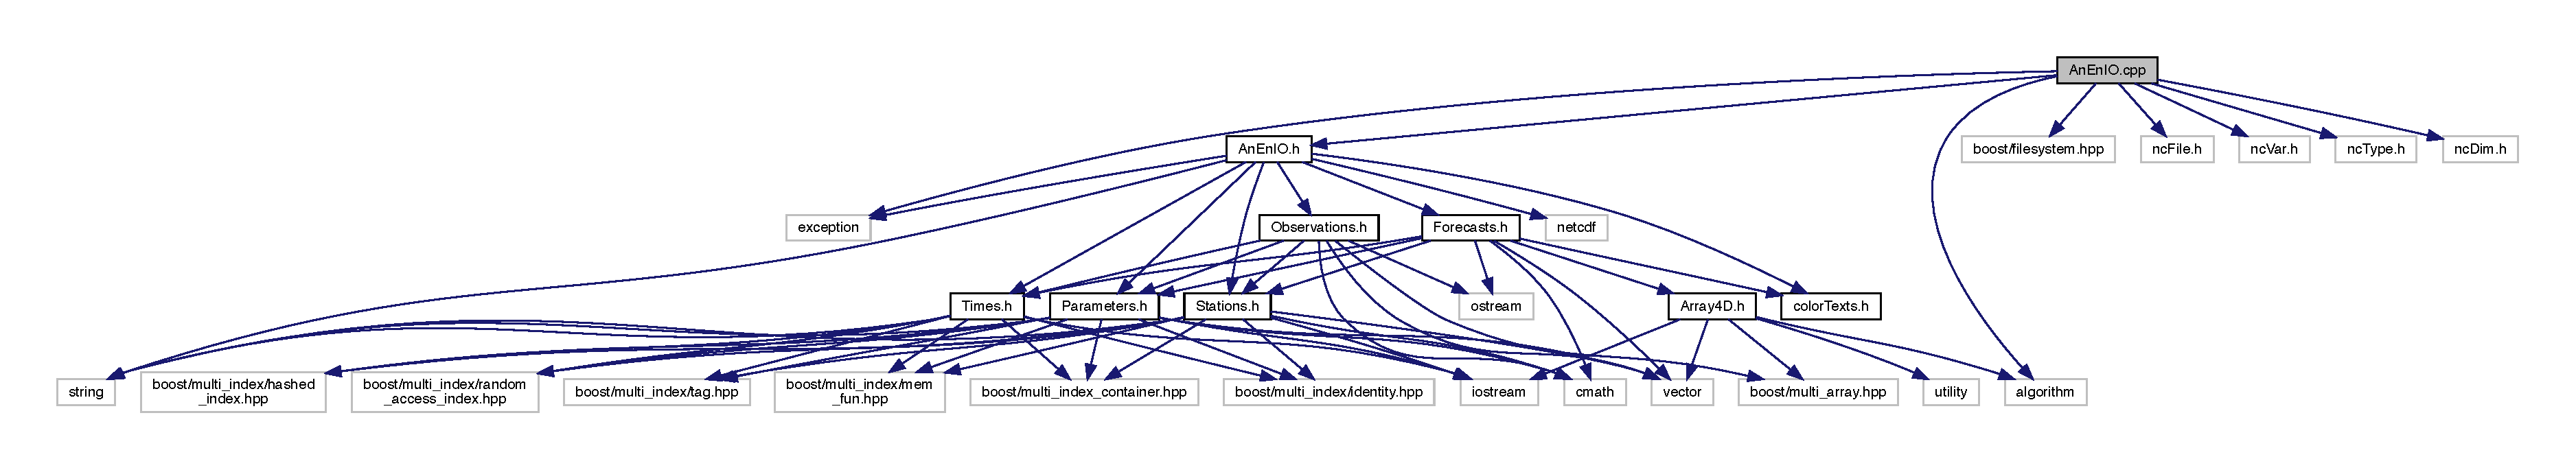
\includegraphics[width=350pt]{_an_en_i_o_8cpp__incl}
\end{center}
\end{figure}
\subsection*{Typedefs}
\begin{DoxyCompactItemize}
\item 
using \mbox{\hyperlink{_an_en_i_o_8cpp_a457b88f1b202c1655ec9a66ab3b4b5e0}{error\+Type}} = \mbox{\hyperlink{class_an_en_i_o_aa56bc1ec6610b86db4349bce20f9ead0}{An\+En\+I\+O\+::error\+Type}}
\end{DoxyCompactItemize}
\subsection*{Variables}
\begin{DoxyCompactItemize}
\item 
size\+\_\+t \mbox{\hyperlink{_an_en_i_o_8cpp_a4239c701053b7ba33c9d94270c2c7028}{\+\_\+max\+\_\+chars}} = 50
\end{DoxyCompactItemize}


\subsection{Typedef Documentation}
\mbox{\Hypertarget{_an_en_i_o_8cpp_a457b88f1b202c1655ec9a66ab3b4b5e0}\label{_an_en_i_o_8cpp_a457b88f1b202c1655ec9a66ab3b4b5e0}} 
\index{An\+En\+I\+O.\+cpp@{An\+En\+I\+O.\+cpp}!error\+Type@{error\+Type}}
\index{error\+Type@{error\+Type}!An\+En\+I\+O.\+cpp@{An\+En\+I\+O.\+cpp}}
\subsubsection{\texorpdfstring{error\+Type}{errorType}}
{\footnotesize\ttfamily using \mbox{\hyperlink{class_an_en_a0e256eb89d102d318a47d936b02242bf}{error\+Type}} =  \mbox{\hyperlink{class_an_en_i_o_aa56bc1ec6610b86db4349bce20f9ead0}{An\+En\+I\+O\+::error\+Type}}}



\subsection{Variable Documentation}
\mbox{\Hypertarget{_an_en_i_o_8cpp_a4239c701053b7ba33c9d94270c2c7028}\label{_an_en_i_o_8cpp_a4239c701053b7ba33c9d94270c2c7028}} 
\index{An\+En\+I\+O.\+cpp@{An\+En\+I\+O.\+cpp}!\+\_\+max\+\_\+chars@{\+\_\+max\+\_\+chars}}
\index{\+\_\+max\+\_\+chars@{\+\_\+max\+\_\+chars}!An\+En\+I\+O.\+cpp@{An\+En\+I\+O.\+cpp}}
\subsubsection{\texorpdfstring{\+\_\+max\+\_\+chars}{\_max\_chars}}
{\footnotesize\ttfamily size\+\_\+t \+\_\+max\+\_\+chars = 50}


\hypertarget{_an_en_i_o_8h}{}\section{An\+En\+I\+O.\+h File Reference}
\label{_an_en_i_o_8h}\index{An\+En\+I\+O.\+h@{An\+En\+I\+O.\+h}}
{\ttfamily \#include $<$netcdf$>$}\newline
{\ttfamily \#include $<$string$>$}\newline
{\ttfamily \#include $<$exception$>$}\newline
{\ttfamily \#include \char`\"{}Times.\+h\char`\"{}}\newline
{\ttfamily \#include \char`\"{}Stations.\+h\char`\"{}}\newline
{\ttfamily \#include \char`\"{}Parameters.\+h\char`\"{}}\newline
{\ttfamily \#include \char`\"{}Forecasts.\+h\char`\"{}}\newline
{\ttfamily \#include \char`\"{}Observations.\+h\char`\"{}}\newline
{\ttfamily \#include \char`\"{}color\+Texts.\+h\char`\"{}}\newline
Include dependency graph for An\+En\+I\+O.\+h\+:
\nopagebreak
\begin{figure}[H]
\begin{center}
\leavevmode
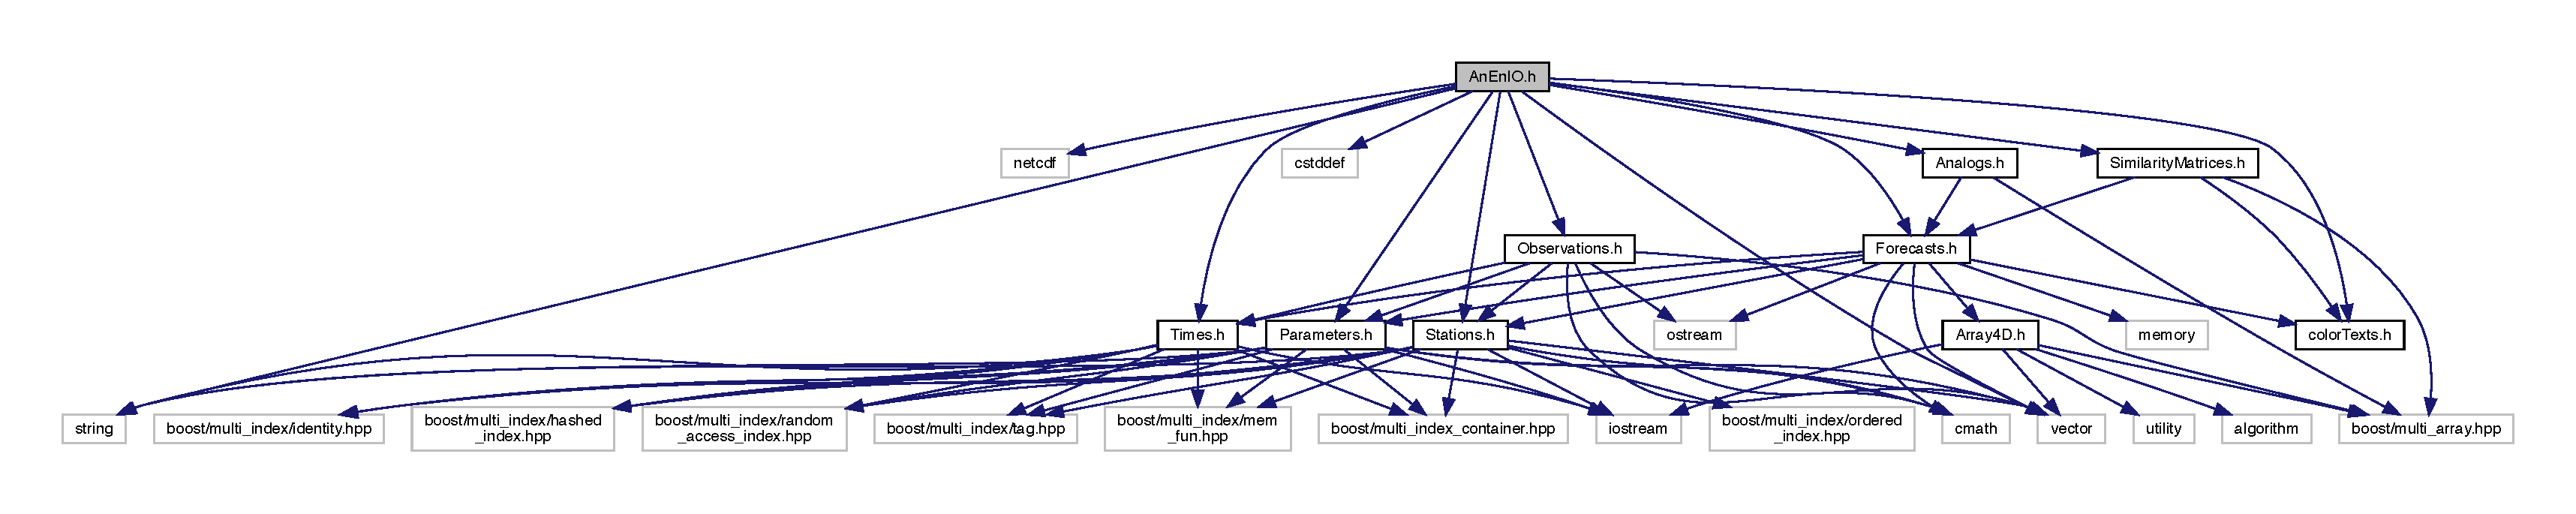
\includegraphics[width=350pt]{_an_en_i_o_8h__incl}
\end{center}
\end{figure}
This graph shows which files directly or indirectly include this file\+:
\nopagebreak
\begin{figure}[H]
\begin{center}
\leavevmode
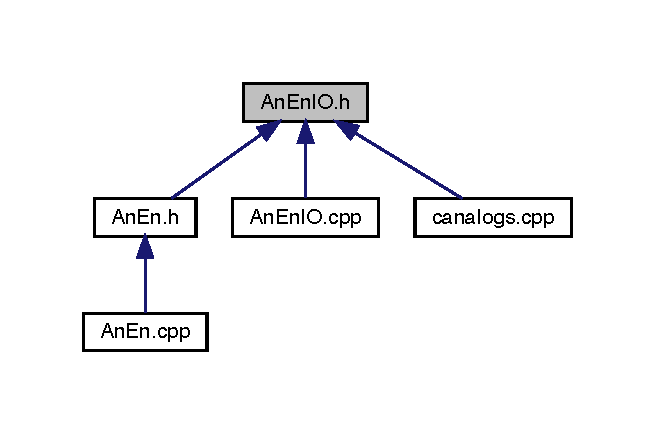
\includegraphics[width=314pt]{_an_en_i_o_8h__dep__incl}
\end{center}
\end{figure}
\subsection*{Classes}
\begin{DoxyCompactItemize}
\item 
class \mbox{\hyperlink{class_an_en_i_o}{An\+En\+IO}}
\begin{DoxyCompactList}\small\item\em \mbox{\hyperlink{class_an_en_i_o}{An\+En\+IO}} class provides interfaces for reading and writing Net\+C\+DF files in forecast, observation, and prediction format. These formats are predefined for generating predictions. \end{DoxyCompactList}\end{DoxyCompactItemize}

\hypertarget{_array4_d_8cpp}{}\section{Array4\+D.\+cpp File Reference}
\label{_array4_d_8cpp}\index{Array4\+D.\+cpp@{Array4\+D.\+cpp}}
{\ttfamily \#include $<$fstream$>$}\newline
{\ttfamily \#include $<$iostream$>$}\newline
{\ttfamily \#include $<$algorithm$>$}\newline
{\ttfamily \#include $<$iterator$>$}\newline
{\ttfamily \#include $<$cstdlib$>$}\newline
{\ttfamily \#include $<$ctime$>$}\newline
{\ttfamily \#include $<$vector$>$}\newline
{\ttfamily \#include \char`\"{}Array4\+D.\+h\char`\"{}}\newline
Include dependency graph for Array4\+D.\+cpp\+:
\nopagebreak
\begin{figure}[H]
\begin{center}
\leavevmode
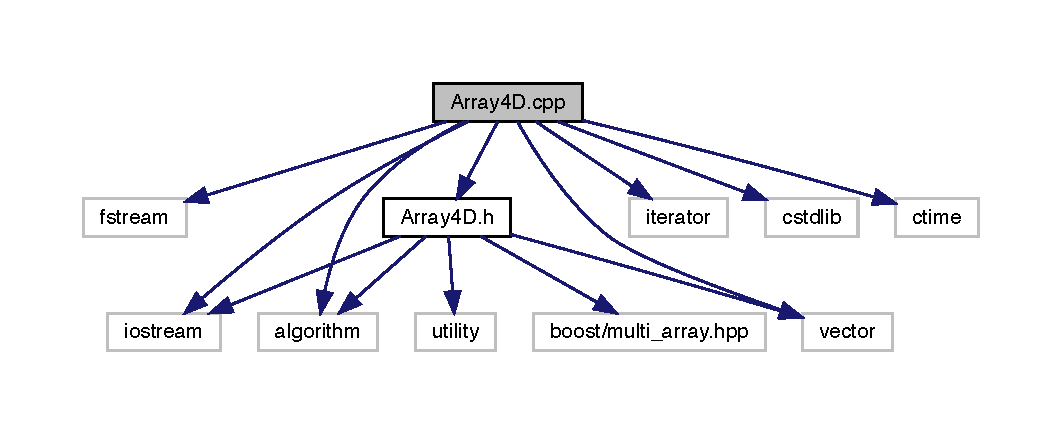
\includegraphics[width=350pt]{_array4_d_8cpp__incl}
\end{center}
\end{figure}
\subsection*{Functions}
\begin{DoxyCompactItemize}
\item 
ostream \& \mbox{\hyperlink{_array4_d_8cpp_aeebfb332d403a9310e7c68f01abff472}{operator$<$$<$}} (ostream \&os, \mbox{\hyperlink{class_array4_d}{Array4D}} const \&bv)
\end{DoxyCompactItemize}


\subsection{Function Documentation}
\mbox{\Hypertarget{_array4_d_8cpp_aeebfb332d403a9310e7c68f01abff472}\label{_array4_d_8cpp_aeebfb332d403a9310e7c68f01abff472}} 
\index{Array4\+D.\+cpp@{Array4\+D.\+cpp}!operator$<$$<$@{operator$<$$<$}}
\index{operator$<$$<$@{operator$<$$<$}!Array4\+D.\+cpp@{Array4\+D.\+cpp}}
\subsubsection{\texorpdfstring{operator$<$$<$()}{operator<<()}}
{\footnotesize\ttfamily ostream\& operator$<$$<$ (\begin{DoxyParamCaption}\item[{ostream \&}]{os,  }\item[{\mbox{\hyperlink{class_array4_d}{Array4D}} const \&}]{bv }\end{DoxyParamCaption})}


\hypertarget{_array4_d_8h}{}\section{Array4\+D.\+h File Reference}
\label{_array4_d_8h}\index{Array4\+D.\+h@{Array4\+D.\+h}}
{\ttfamily \#include \char`\"{}boost/multi\+\_\+array.\+hpp\char`\"{}}\newline
{\ttfamily \#include $<$iostream$>$}\newline
{\ttfamily \#include $<$vector$>$}\newline
{\ttfamily \#include $<$utility$>$}\newline
{\ttfamily \#include $<$algorithm$>$}\newline
Include dependency graph for Array4\+D.\+h\+:\nopagebreak
\begin{figure}[H]
\begin{center}
\leavevmode
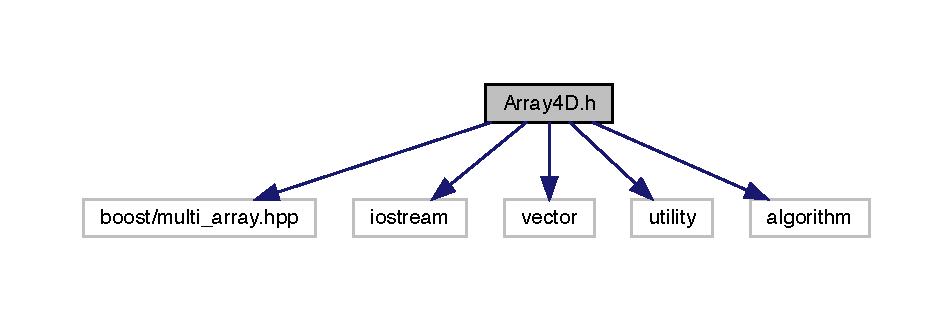
\includegraphics[width=350pt]{_array4_d_8h__incl}
\end{center}
\end{figure}
This graph shows which files directly or indirectly include this file\+:
\nopagebreak
\begin{figure}[H]
\begin{center}
\leavevmode
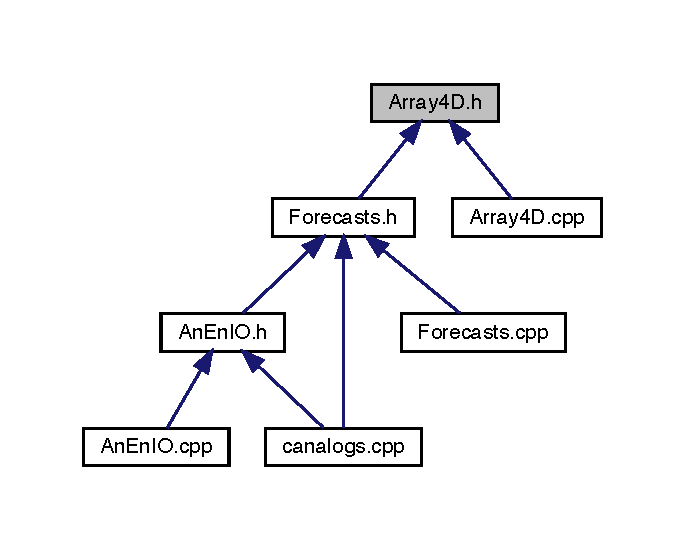
\includegraphics[width=350pt]{_array4_d_8h__dep__incl}
\end{center}
\end{figure}
\subsection*{Classes}
\begin{DoxyCompactItemize}
\item 
class \mbox{\hyperlink{class_array4_d}{Array4D}}
\end{DoxyCompactItemize}

\hypertarget{canalogs_8cpp}{}\section{canalogs.\+cpp File Reference}
\label{canalogs_8cpp}\index{canalogs.\+cpp@{canalogs.\+cpp}}
{\ttfamily \#include $<$cstdlib$>$}\newline
{\ttfamily \#include $<$string$>$}\newline
{\ttfamily \#include \char`\"{}Stations.\+h\char`\"{}}\newline
{\ttfamily \#include \char`\"{}Parameters.\+h\char`\"{}}\newline
{\ttfamily \#include \char`\"{}Times.\+h\char`\"{}}\newline
{\ttfamily \#include \char`\"{}Forecasts.\+h\char`\"{}}\newline
{\ttfamily \#include \char`\"{}An\+En\+I\+O.\+h\char`\"{}}\newline
Include dependency graph for canalogs.\+cpp\+:
\nopagebreak
\begin{figure}[H]
\begin{center}
\leavevmode
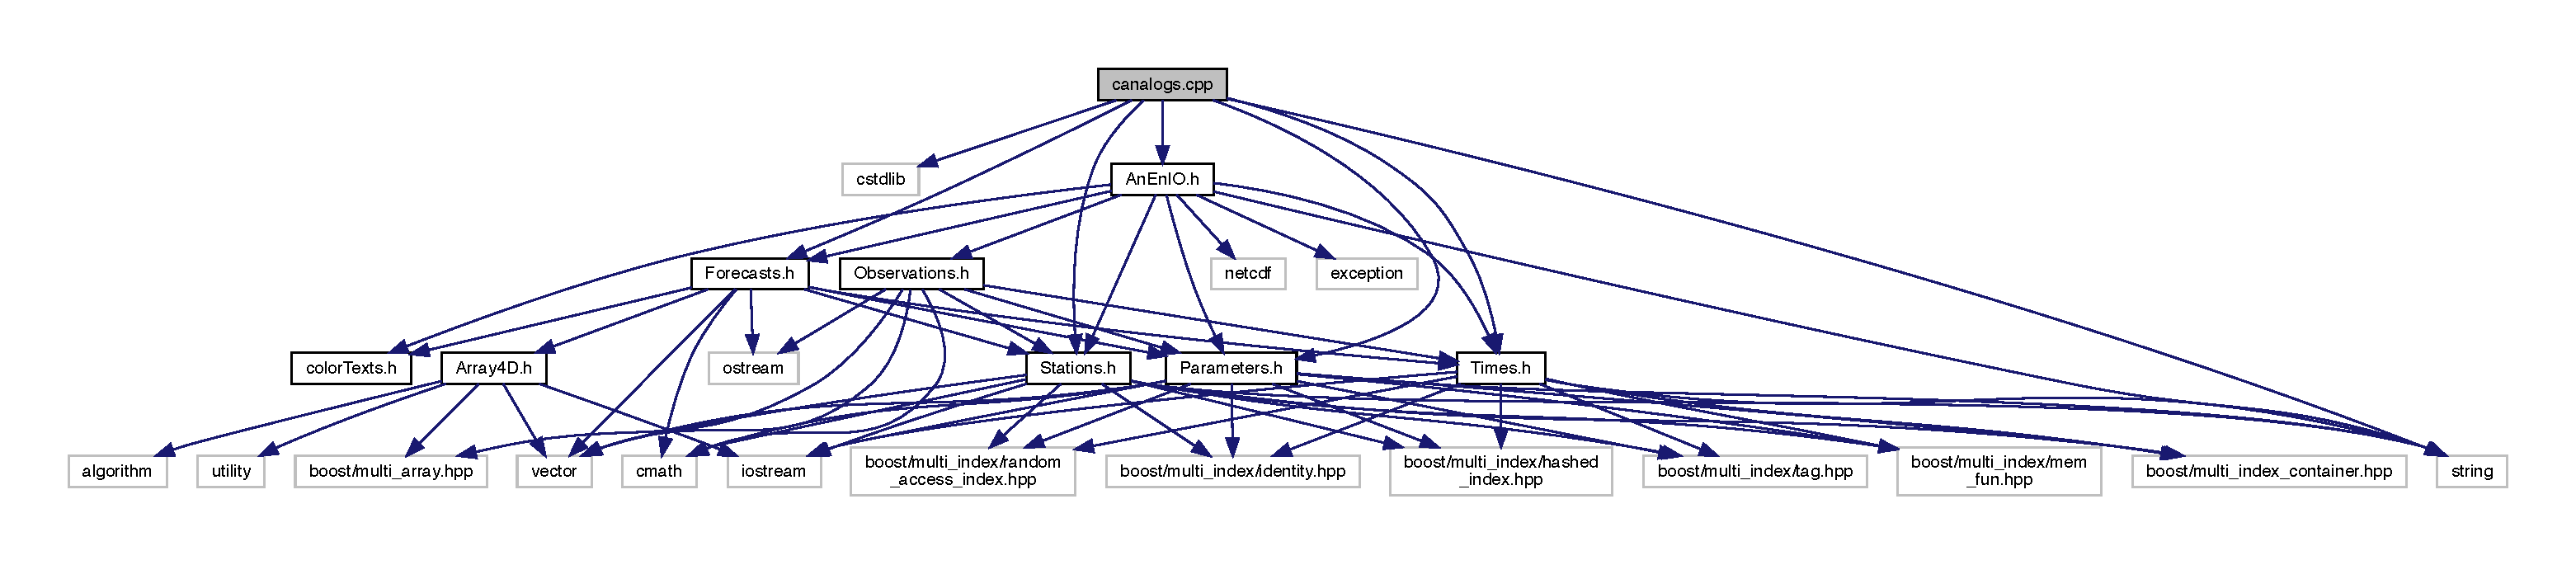
\includegraphics[width=350pt]{canalogs_8cpp__incl}
\end{center}
\end{figure}
\subsection*{Functions}
\begin{DoxyCompactItemize}
\item 
int \mbox{\hyperlink{canalogs_8cpp_a3c04138a5bfe5d72780bb7e82a18e627}{main}} (int argc, char $\ast$$\ast$argv)
\end{DoxyCompactItemize}


\subsection{Function Documentation}
\mbox{\Hypertarget{canalogs_8cpp_a3c04138a5bfe5d72780bb7e82a18e627}\label{canalogs_8cpp_a3c04138a5bfe5d72780bb7e82a18e627}} 
\index{canalogs.\+cpp@{canalogs.\+cpp}!main@{main}}
\index{main@{main}!canalogs.\+cpp@{canalogs.\+cpp}}
\subsubsection{\texorpdfstring{main()}{main()}}
{\footnotesize\ttfamily int main (\begin{DoxyParamCaption}\item[{int}]{argc,  }\item[{char $\ast$$\ast$}]{argv }\end{DoxyParamCaption})}


\hypertarget{color_texts_8h}{}\section{color\+Texts.\+h File Reference}
\label{color_texts_8h}\index{color\+Texts.\+h@{color\+Texts.\+h}}
This graph shows which files directly or indirectly include this file\+:
\nopagebreak
\begin{figure}[H]
\begin{center}
\leavevmode
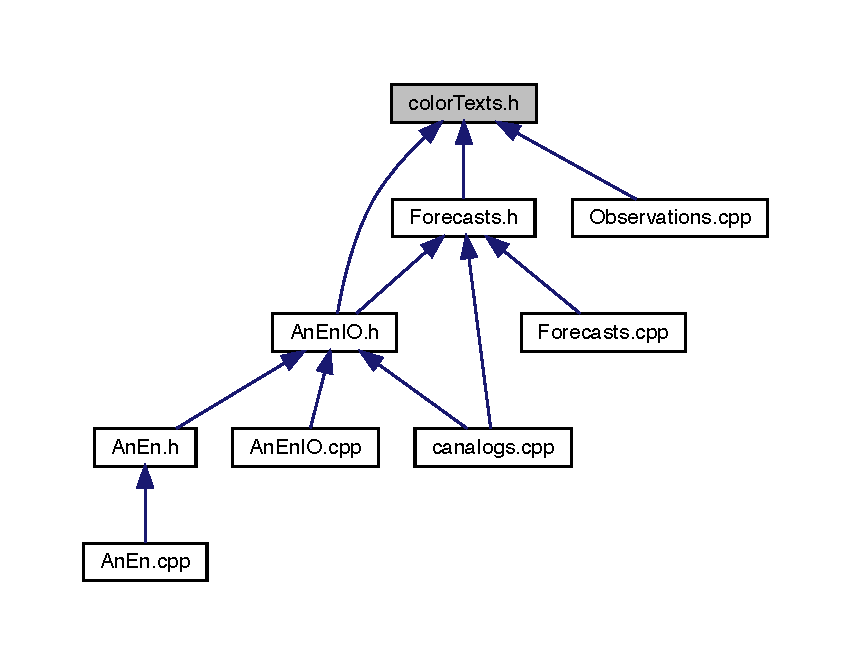
\includegraphics[width=242pt]{color_texts_8h__dep__incl}
\end{center}
\end{figure}
\subsection*{Macros}
\begin{DoxyCompactItemize}
\item 
\#define \mbox{\hyperlink{color_texts_8h_ab702106cf3b3e96750b6845ded4e0299}{R\+E\+S\+ET}}~\char`\"{}\textbackslash{}033\mbox{[}0m\char`\"{}
\item 
\#define \mbox{\hyperlink{color_texts_8h_ab912d02c7998c3d47d05f87be4e2c920}{B\+O\+L\+D\+R\+ED}}~\char`\"{}\textbackslash{}033\mbox{[}1m\textbackslash{}033\mbox{[}31m\char`\"{}
\item 
\#define \mbox{\hyperlink{color_texts_8h_a4a6c893a1703c33ede7d702fe5f97c91}{B\+O\+L\+D\+G\+R\+E\+EN}}~\char`\"{}\textbackslash{}033\mbox{[}1m\textbackslash{}033\mbox{[}32m\char`\"{}
\item 
\#define \mbox{\hyperlink{color_texts_8h_a8d23feea868a983c8c2b661e1e16972f}{R\+ED}}~\char`\"{}\textbackslash{}033\mbox{[}31m\char`\"{}
\item 
\#define \mbox{\hyperlink{color_texts_8h_acfbc006ea433ad708fdee3e82996e721}{G\+R\+E\+EN}}~\char`\"{}\textbackslash{}033\mbox{[}32m\char`\"{}
\end{DoxyCompactItemize}


\subsection{Macro Definition Documentation}
\mbox{\Hypertarget{color_texts_8h_a4a6c893a1703c33ede7d702fe5f97c91}\label{color_texts_8h_a4a6c893a1703c33ede7d702fe5f97c91}} 
\index{color\+Texts.\+h@{color\+Texts.\+h}!B\+O\+L\+D\+G\+R\+E\+EN@{B\+O\+L\+D\+G\+R\+E\+EN}}
\index{B\+O\+L\+D\+G\+R\+E\+EN@{B\+O\+L\+D\+G\+R\+E\+EN}!color\+Texts.\+h@{color\+Texts.\+h}}
\subsubsection{\texorpdfstring{B\+O\+L\+D\+G\+R\+E\+EN}{BOLDGREEN}}
{\footnotesize\ttfamily \#define B\+O\+L\+D\+G\+R\+E\+EN~\char`\"{}\textbackslash{}033\mbox{[}1m\textbackslash{}033\mbox{[}32m\char`\"{}}

\mbox{\Hypertarget{color_texts_8h_ab912d02c7998c3d47d05f87be4e2c920}\label{color_texts_8h_ab912d02c7998c3d47d05f87be4e2c920}} 
\index{color\+Texts.\+h@{color\+Texts.\+h}!B\+O\+L\+D\+R\+ED@{B\+O\+L\+D\+R\+ED}}
\index{B\+O\+L\+D\+R\+ED@{B\+O\+L\+D\+R\+ED}!color\+Texts.\+h@{color\+Texts.\+h}}
\subsubsection{\texorpdfstring{B\+O\+L\+D\+R\+ED}{BOLDRED}}
{\footnotesize\ttfamily \#define B\+O\+L\+D\+R\+ED~\char`\"{}\textbackslash{}033\mbox{[}1m\textbackslash{}033\mbox{[}31m\char`\"{}}

\mbox{\Hypertarget{color_texts_8h_acfbc006ea433ad708fdee3e82996e721}\label{color_texts_8h_acfbc006ea433ad708fdee3e82996e721}} 
\index{color\+Texts.\+h@{color\+Texts.\+h}!G\+R\+E\+EN@{G\+R\+E\+EN}}
\index{G\+R\+E\+EN@{G\+R\+E\+EN}!color\+Texts.\+h@{color\+Texts.\+h}}
\subsubsection{\texorpdfstring{G\+R\+E\+EN}{GREEN}}
{\footnotesize\ttfamily \#define G\+R\+E\+EN~\char`\"{}\textbackslash{}033\mbox{[}32m\char`\"{}}

\mbox{\Hypertarget{color_texts_8h_a8d23feea868a983c8c2b661e1e16972f}\label{color_texts_8h_a8d23feea868a983c8c2b661e1e16972f}} 
\index{color\+Texts.\+h@{color\+Texts.\+h}!R\+ED@{R\+ED}}
\index{R\+ED@{R\+ED}!color\+Texts.\+h@{color\+Texts.\+h}}
\subsubsection{\texorpdfstring{R\+ED}{RED}}
{\footnotesize\ttfamily \#define R\+ED~\char`\"{}\textbackslash{}033\mbox{[}31m\char`\"{}}

\mbox{\Hypertarget{color_texts_8h_ab702106cf3b3e96750b6845ded4e0299}\label{color_texts_8h_ab702106cf3b3e96750b6845ded4e0299}} 
\index{color\+Texts.\+h@{color\+Texts.\+h}!R\+E\+S\+ET@{R\+E\+S\+ET}}
\index{R\+E\+S\+ET@{R\+E\+S\+ET}!color\+Texts.\+h@{color\+Texts.\+h}}
\subsubsection{\texorpdfstring{R\+E\+S\+ET}{RESET}}
{\footnotesize\ttfamily \#define R\+E\+S\+ET~\char`\"{}\textbackslash{}033\mbox{[}0m\char`\"{}}


\hypertarget{_forecasts_8cpp}{}\section{Forecasts.\+cpp File Reference}
\label{_forecasts_8cpp}\index{Forecasts.\+cpp@{Forecasts.\+cpp}}
{\ttfamily \#include \char`\"{}Forecasts.\+h\char`\"{}}\newline
Include dependency graph for Forecasts.\+cpp\+:
\nopagebreak
\begin{figure}[H]
\begin{center}
\leavevmode
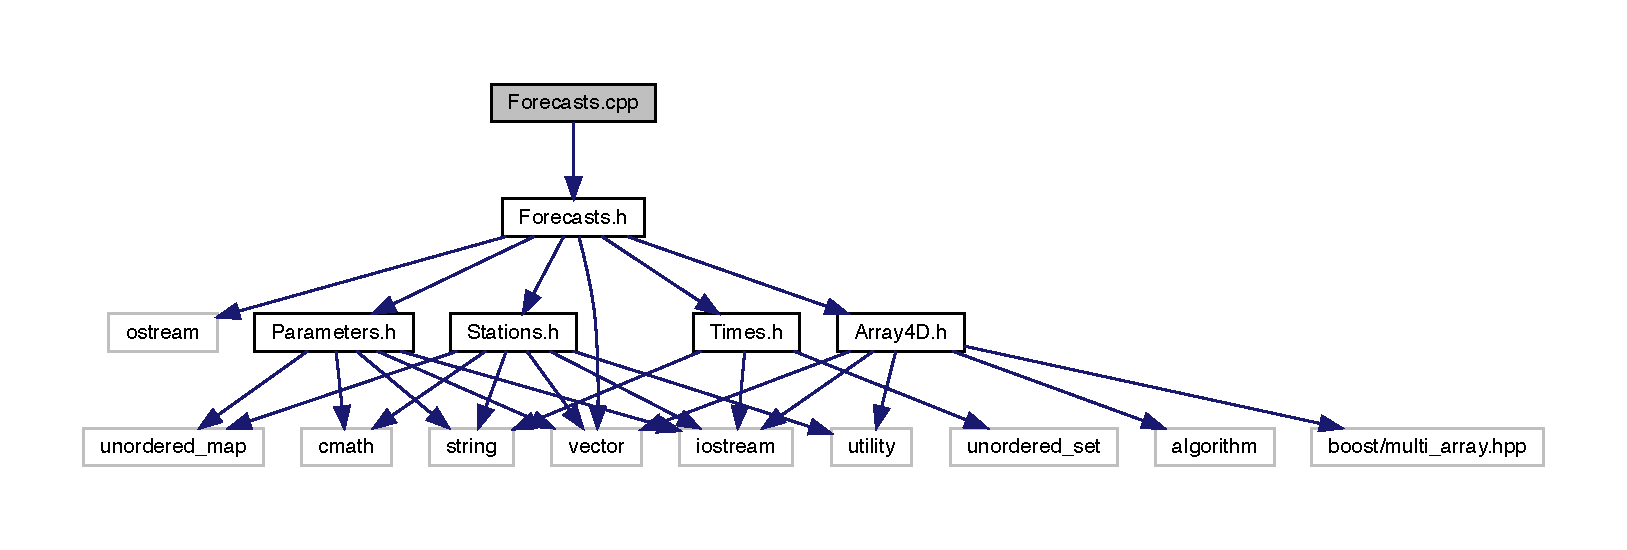
\includegraphics[width=350pt]{_forecasts_8cpp__incl}
\end{center}
\end{figure}
\subsection*{Functions}
\begin{DoxyCompactItemize}
\item 
ostream \& \mbox{\hyperlink{_forecasts_8cpp_a89762c07ae9b9c571f0382716163b4be}{operator$<$$<$}} (ostream \&os, \mbox{\hyperlink{class_forecasts}{Forecasts}} const \&obj)
\item 
ostream \& \mbox{\hyperlink{_forecasts_8cpp_abd4473b173972ce91b5f624750179d6b}{operator$<$$<$}} (ostream \&os, const \mbox{\hyperlink{class_forecasts__array}{Forecasts\+\_\+array}} \&obj)
\end{DoxyCompactItemize}


\subsection{Function Documentation}
\mbox{\Hypertarget{_forecasts_8cpp_a89762c07ae9b9c571f0382716163b4be}\label{_forecasts_8cpp_a89762c07ae9b9c571f0382716163b4be}} 
\index{Forecasts.\+cpp@{Forecasts.\+cpp}!operator$<$$<$@{operator$<$$<$}}
\index{operator$<$$<$@{operator$<$$<$}!Forecasts.\+cpp@{Forecasts.\+cpp}}
\subsubsection{\texorpdfstring{operator$<$$<$()}{operator<<()}\hspace{0.1cm}{\footnotesize\ttfamily [1/2]}}
{\footnotesize\ttfamily ostream\& operator$<$$<$ (\begin{DoxyParamCaption}\item[{ostream \&}]{os,  }\item[{\mbox{\hyperlink{class_forecasts}{Forecasts}} const \&}]{obj }\end{DoxyParamCaption})}

\mbox{\Hypertarget{_forecasts_8cpp_abd4473b173972ce91b5f624750179d6b}\label{_forecasts_8cpp_abd4473b173972ce91b5f624750179d6b}} 
\index{Forecasts.\+cpp@{Forecasts.\+cpp}!operator$<$$<$@{operator$<$$<$}}
\index{operator$<$$<$@{operator$<$$<$}!Forecasts.\+cpp@{Forecasts.\+cpp}}
\subsubsection{\texorpdfstring{operator$<$$<$()}{operator<<()}\hspace{0.1cm}{\footnotesize\ttfamily [2/2]}}
{\footnotesize\ttfamily ostream\& operator$<$$<$ (\begin{DoxyParamCaption}\item[{ostream \&}]{os,  }\item[{const \mbox{\hyperlink{class_forecasts__array}{Forecasts\+\_\+array}} \&}]{obj }\end{DoxyParamCaption})}


\hypertarget{_forecasts_8h}{}\section{Forecasts.\+h File Reference}
\label{_forecasts_8h}\index{Forecasts.\+h@{Forecasts.\+h}}
{\ttfamily \#include $<$ostream$>$}\newline
{\ttfamily \#include $<$cmath$>$}\newline
{\ttfamily \#include $<$vector$>$}\newline
{\ttfamily \#include \char`\"{}Stations.\+h\char`\"{}}\newline
{\ttfamily \#include \char`\"{}Parameters.\+h\char`\"{}}\newline
{\ttfamily \#include \char`\"{}Times.\+h\char`\"{}}\newline
{\ttfamily \#include \char`\"{}Array4\+D.\+h\char`\"{}}\newline
Include dependency graph for Forecasts.\+h\+:\nopagebreak
\begin{figure}[H]
\begin{center}
\leavevmode
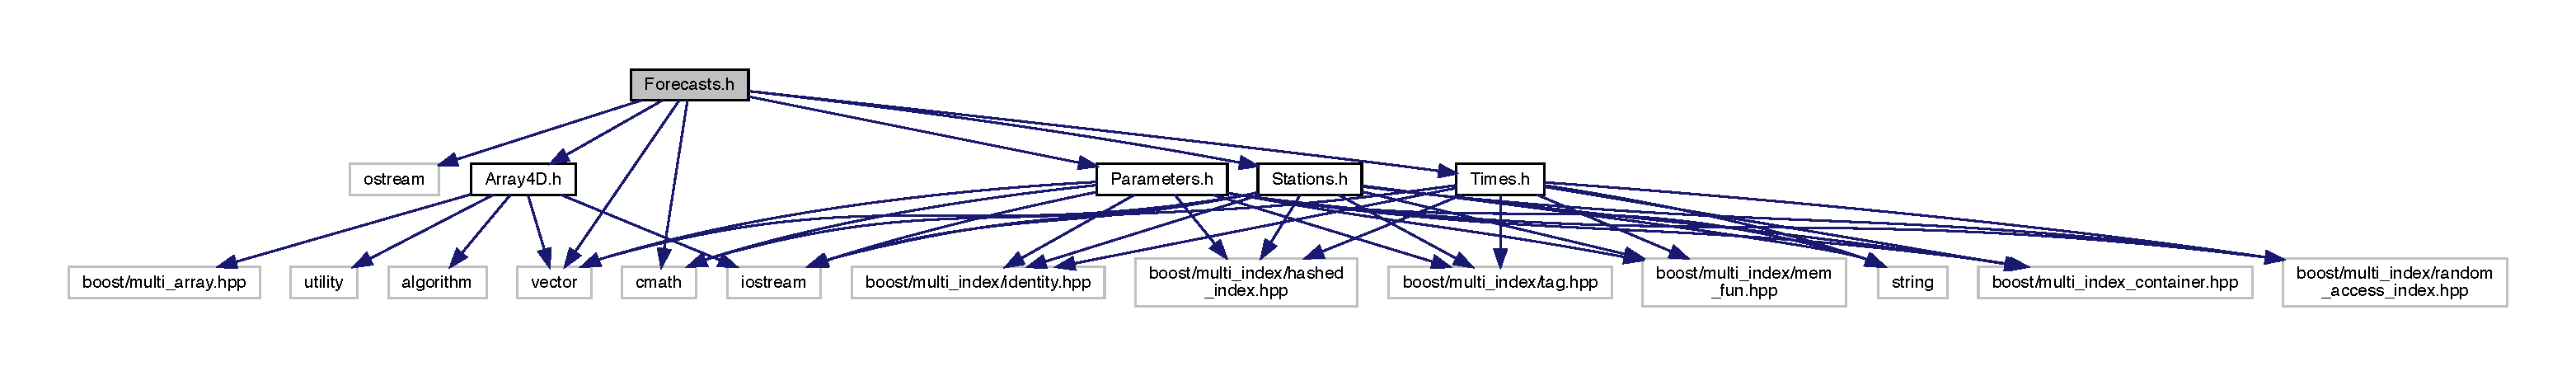
\includegraphics[width=350pt]{_forecasts_8h__incl}
\end{center}
\end{figure}
This graph shows which files directly or indirectly include this file\+:\nopagebreak
\begin{figure}[H]
\begin{center}
\leavevmode
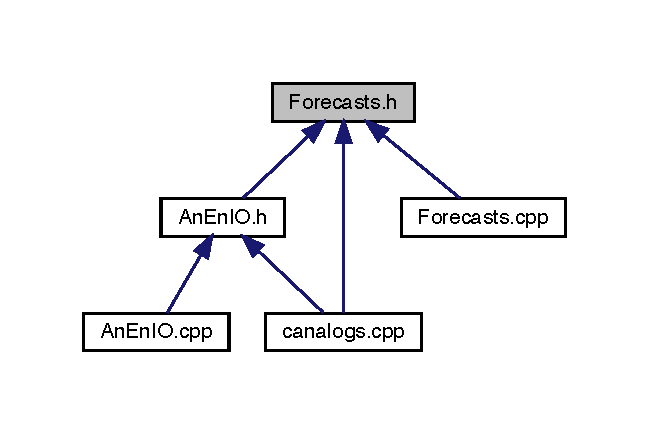
\includegraphics[width=311pt]{_forecasts_8h__dep__incl}
\end{center}
\end{figure}
\subsection*{Classes}
\begin{DoxyCompactItemize}
\item 
class \mbox{\hyperlink{class_forecasts}{Forecasts}}
\begin{DoxyCompactList}\small\item\em \mbox{\hyperlink{class_forecasts}{Forecasts}} class provides interface for reading and writing forecast data from and to a Net\+C\+DF file. It also supports data indexing and searching. \end{DoxyCompactList}\item 
class \mbox{\hyperlink{class_forecasts__array}{Forecasts\+\_\+array}}
\begin{DoxyCompactList}\small\item\em \mbox{\hyperlink{class_forecasts__array}{Forecasts\+\_\+array}} class is an implementation of class \mbox{\hyperlink{class_forecasts}{Forecasts}}. Data are stored using the \mbox{\hyperlink{class_array4_d}{Array4D}} class. \end{DoxyCompactList}\end{DoxyCompactItemize}

\hypertarget{_observations_8cpp}{}\section{Observations.\+cpp File Reference}
\label{_observations_8cpp}\index{Observations.\+cpp@{Observations.\+cpp}}
{\ttfamily \#include \char`\"{}Observations.\+h\char`\"{}}\newline
{\ttfamily \#include $<$stdexcept$>$}\newline
{\ttfamily \#include $<$algorithm$>$}\newline
Include dependency graph for Observations.\+cpp\+:\nopagebreak
\begin{figure}[H]
\begin{center}
\leavevmode
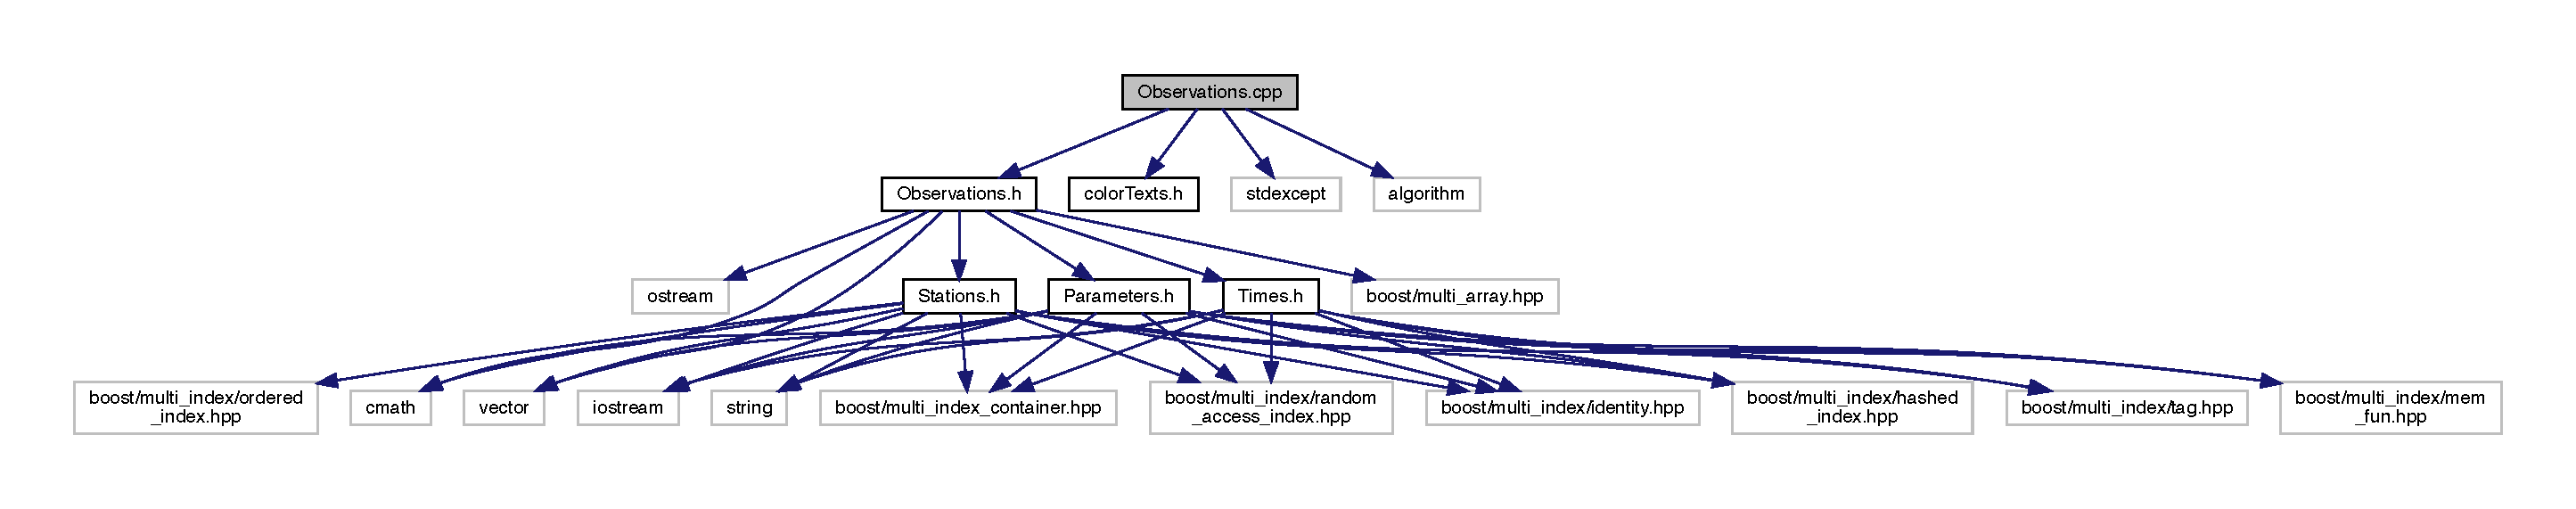
\includegraphics[width=350pt]{_observations_8cpp__incl}
\end{center}
\end{figure}
\subsection*{Functions}
\begin{DoxyCompactItemize}
\item 
ostream \& \mbox{\hyperlink{_observations_8cpp_a91ccfa64dbd9051fc34bc6bf3da6926f}{operator$<$$<$}} (ostream \&os, const \mbox{\hyperlink{class_observations}{Observations}} \&obj)
\item 
ostream \& \mbox{\hyperlink{_observations_8cpp_adca8c38e40482680b9e43ab256cad034}{operator$<$$<$}} (ostream \&os, const \mbox{\hyperlink{class_observations__array}{Observations\+\_\+array}} \&obj)
\end{DoxyCompactItemize}


\subsection{Function Documentation}
\mbox{\Hypertarget{_observations_8cpp_a91ccfa64dbd9051fc34bc6bf3da6926f}\label{_observations_8cpp_a91ccfa64dbd9051fc34bc6bf3da6926f}} 
\index{Observations.\+cpp@{Observations.\+cpp}!operator$<$$<$@{operator$<$$<$}}
\index{operator$<$$<$@{operator$<$$<$}!Observations.\+cpp@{Observations.\+cpp}}
\subsubsection{\texorpdfstring{operator$<$$<$()}{operator<<()}\hspace{0.1cm}{\footnotesize\ttfamily [1/2]}}
{\footnotesize\ttfamily ostream\& operator$<$$<$ (\begin{DoxyParamCaption}\item[{ostream \&}]{os,  }\item[{const \mbox{\hyperlink{class_observations}{Observations}} \&}]{obj }\end{DoxyParamCaption})}

\mbox{\Hypertarget{_observations_8cpp_adca8c38e40482680b9e43ab256cad034}\label{_observations_8cpp_adca8c38e40482680b9e43ab256cad034}} 
\index{Observations.\+cpp@{Observations.\+cpp}!operator$<$$<$@{operator$<$$<$}}
\index{operator$<$$<$@{operator$<$$<$}!Observations.\+cpp@{Observations.\+cpp}}
\subsubsection{\texorpdfstring{operator$<$$<$()}{operator<<()}\hspace{0.1cm}{\footnotesize\ttfamily [2/2]}}
{\footnotesize\ttfamily ostream\& operator$<$$<$ (\begin{DoxyParamCaption}\item[{ostream \&}]{os,  }\item[{const \mbox{\hyperlink{class_observations__array}{Observations\+\_\+array}} \&}]{obj }\end{DoxyParamCaption})}


\hypertarget{_observations_8h}{}\section{Observations.\+h File Reference}
\label{_observations_8h}\index{Observations.\+h@{Observations.\+h}}
{\ttfamily \#include $<$ostream$>$}\newline
{\ttfamily \#include $<$vector$>$}\newline
{\ttfamily \#include \char`\"{}Parameters.\+h\char`\"{}}\newline
{\ttfamily \#include \char`\"{}Stations.\+h\char`\"{}}\newline
{\ttfamily \#include \char`\"{}Times.\+h\char`\"{}}\newline
{\ttfamily \#include $<$boost/multi\+\_\+array.\+hpp$>$}\newline
Include dependency graph for Observations.\+h\+:
\nopagebreak
\begin{figure}[H]
\begin{center}
\leavevmode
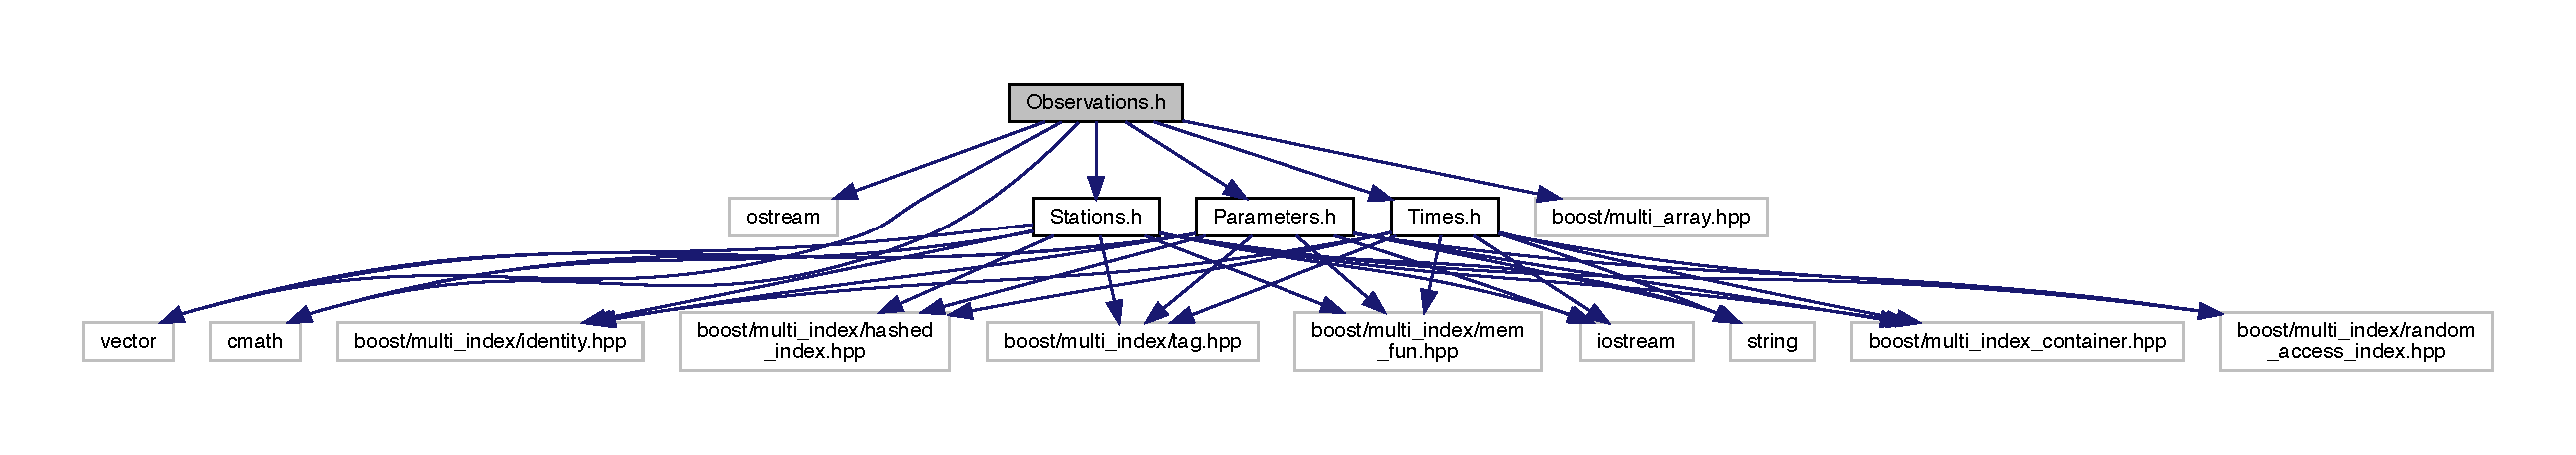
\includegraphics[width=350pt]{_observations_8h__incl}
\end{center}
\end{figure}
This graph shows which files directly or indirectly include this file\+:
\nopagebreak
\begin{figure}[H]
\begin{center}
\leavevmode
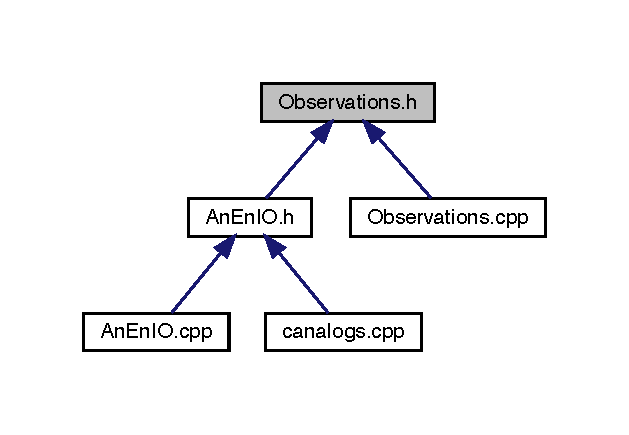
\includegraphics[width=302pt]{_observations_8h__dep__incl}
\end{center}
\end{figure}
\subsection*{Classes}
\begin{DoxyCompactItemize}
\item 
class \mbox{\hyperlink{class_observations}{Observations}}
\item 
class \mbox{\hyperlink{class_observations__array}{Observations\+\_\+array}}
\end{DoxyCompactItemize}

\hypertarget{_parameters_8cpp}{}\section{Parameters.\+cpp File Reference}
\label{_parameters_8cpp}\index{Parameters.\+cpp@{Parameters.\+cpp}}
{\ttfamily \#include \char`\"{}Parameters.\+h\char`\"{}}\newline
{\ttfamily \#include $<$iterator$>$}\newline
Include dependency graph for Parameters.\+cpp\+:\nopagebreak
\begin{figure}[H]
\begin{center}
\leavevmode
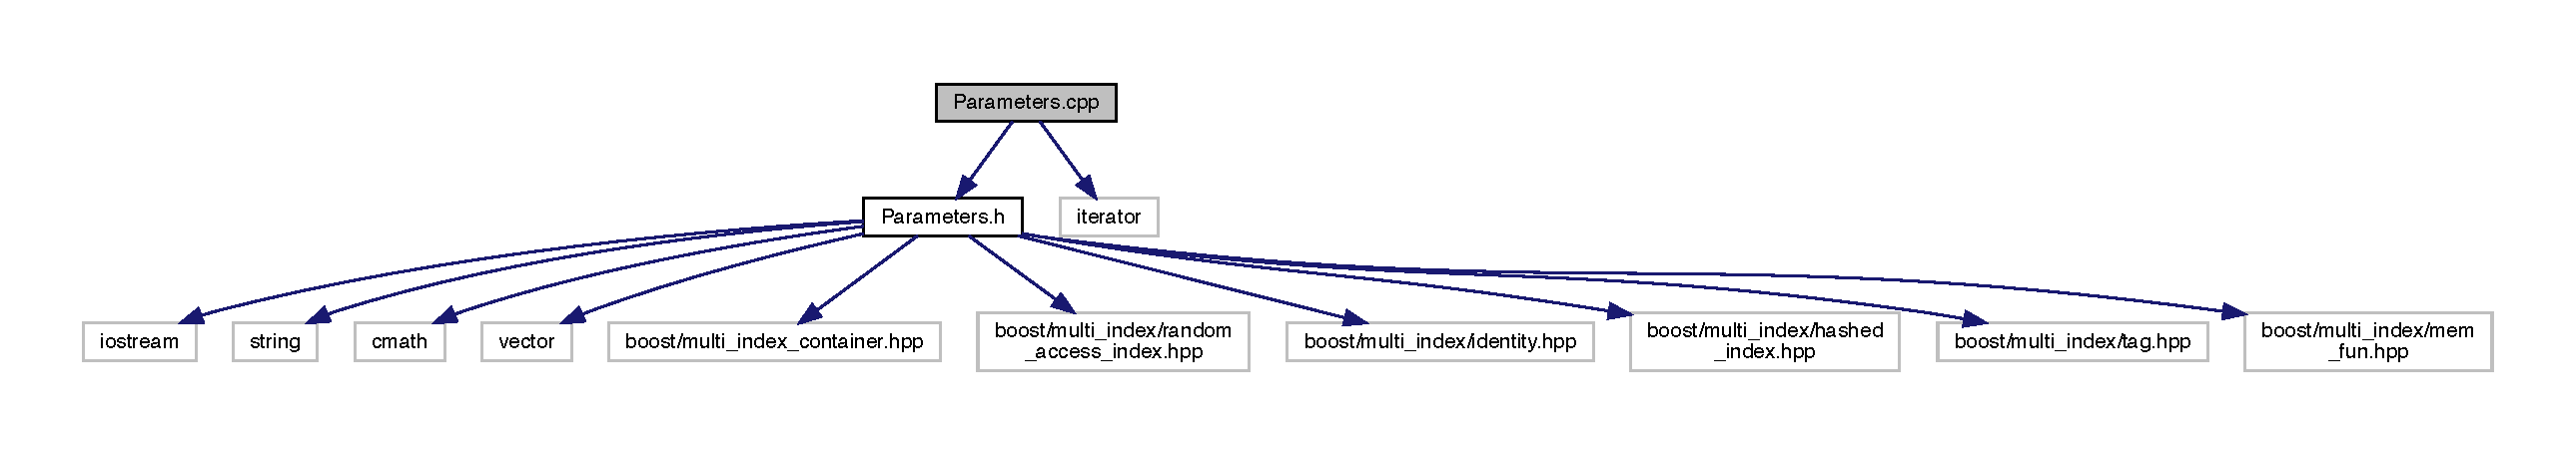
\includegraphics[width=350pt]{_parameters_8cpp__incl}
\end{center}
\end{figure}
\subsection*{Namespaces}
\begin{DoxyCompactItemize}
\item 
 \mbox{\hyperlink{namespaceanen_par}{anen\+Par}}
\end{DoxyCompactItemize}
\subsection*{Functions}
\begin{DoxyCompactItemize}
\item 
ostream \& \mbox{\hyperlink{namespaceanen_par_a52a5a22e980d0d41a493b6cb3f5b0bb4}{anen\+Par\+::operator$<$$<$}} (ostream \&os, Parameter const \&obj)
\item 
ostream \& \mbox{\hyperlink{namespaceanen_par_a670cbfb557a503e08dd170516c81b075}{anen\+Par\+::operator$<$$<$}} (ostream \&os, Parameters const \&obj)
\end{DoxyCompactItemize}

\hypertarget{_parameters_8h}{}\section{Parameters.\+h File Reference}
\label{_parameters_8h}\index{Parameters.\+h@{Parameters.\+h}}
{\ttfamily \#include $<$iostream$>$}\newline
{\ttfamily \#include $<$string$>$}\newline
{\ttfamily \#include $<$cmath$>$}\newline
{\ttfamily \#include $<$vector$>$}\newline
{\ttfamily \#include $<$boost/multi\+\_\+index\+\_\+container.\+hpp$>$}\newline
{\ttfamily \#include $<$boost/multi\+\_\+index/random\+\_\+access\+\_\+index.\+hpp$>$}\newline
{\ttfamily \#include $<$boost/multi\+\_\+index/identity.\+hpp$>$}\newline
{\ttfamily \#include $<$boost/multi\+\_\+index/hashed\+\_\+index.\+hpp$>$}\newline
{\ttfamily \#include $<$boost/multi\+\_\+index/tag.\+hpp$>$}\newline
{\ttfamily \#include $<$boost/multi\+\_\+index/mem\+\_\+fun.\+hpp$>$}\newline
Include dependency graph for Parameters.\+h\+:\nopagebreak
\begin{figure}[H]
\begin{center}
\leavevmode
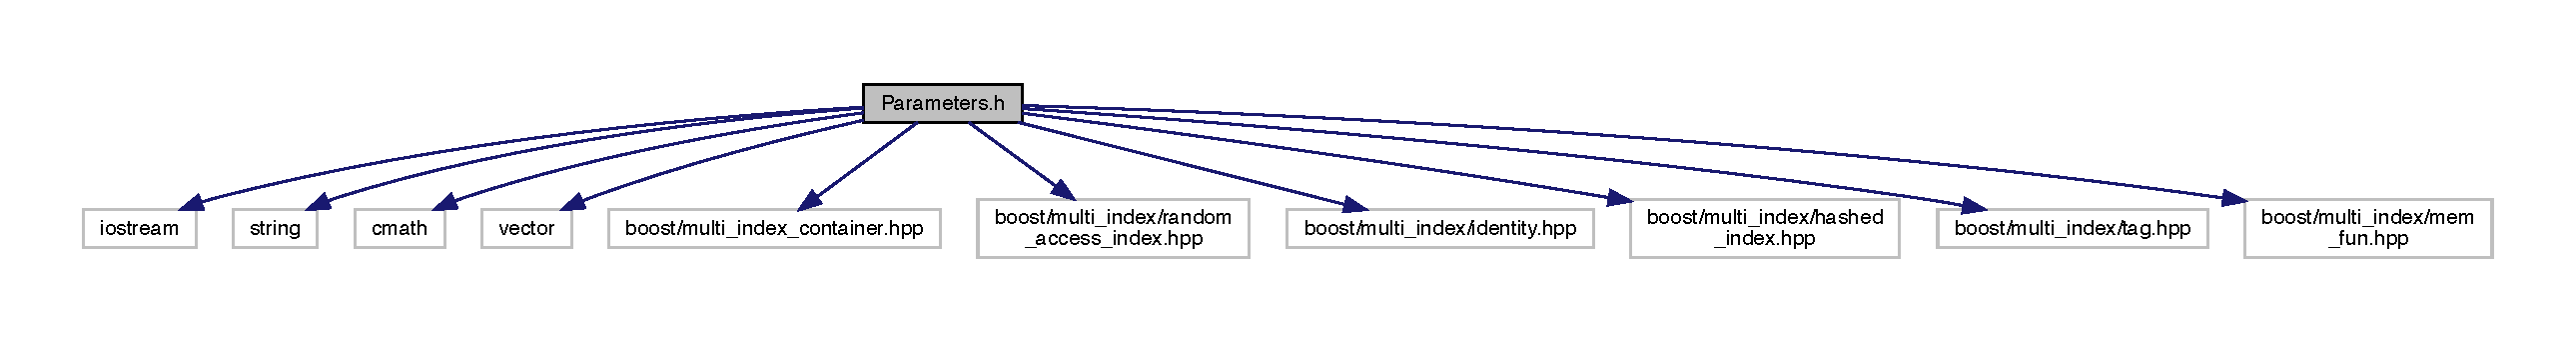
\includegraphics[width=350pt]{_parameters_8h__incl}
\end{center}
\end{figure}
This graph shows which files directly or indirectly include this file\+:
\nopagebreak
\begin{figure}[H]
\begin{center}
\leavevmode
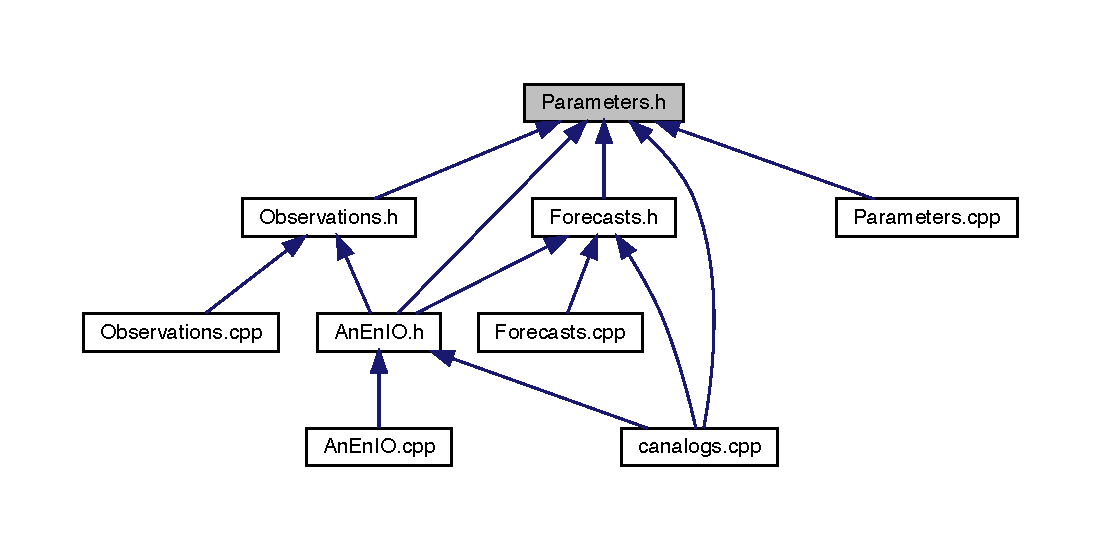
\includegraphics[width=350pt]{_parameters_8h__dep__incl}
\end{center}
\end{figure}
\subsection*{Classes}
\begin{DoxyCompactItemize}
\item 
class \mbox{\hyperlink{classanen_par_1_1_parameter}{anen\+Par\+::\+Parameter}}
\begin{DoxyCompactList}\small\item\em \mbox{\hyperlink{classanen_par_1_1_parameter}{Parameter}} stores parameter information including name, weight, and circular. Each \mbox{\hyperlink{classanen_par_1_1_parameter}{Parameter}} object is assigned with an unique ID. This ID can be useful for parameter retrieval. \end{DoxyCompactList}\item 
struct \mbox{\hyperlink{structanen_par_1_1by__insert}{anen\+Par\+::by\+\_\+insert}}
\item 
struct \mbox{\hyperlink{structanen_par_1_1by___i_d}{anen\+Par\+::by\+\_\+\+ID}}
\item 
class \mbox{\hyperlink{classanen_par_1_1_parameters}{anen\+Par\+::\+Parameters}}
\begin{DoxyCompactList}\small\item\em \mbox{\hyperlink{classanen_par_1_1_parameters}{Parameters}} class stores \mbox{\hyperlink{classanen_par_1_1_parameter}{Parameter}} objects. \end{DoxyCompactList}\end{DoxyCompactItemize}
\subsection*{Namespaces}
\begin{DoxyCompactItemize}
\item 
 \mbox{\hyperlink{namespaceanen_par}{anen\+Par}}
\end{DoxyCompactItemize}
\subsection*{Typedefs}
\begin{DoxyCompactItemize}
\item 
using \mbox{\hyperlink{namespaceanen_par_a80347e56535f3553dead0c9515dbecd6}{anen\+Par\+::multi\+Index\+Parameters}} = boost\+::multi\+\_\+index\+\_\+container$<$ Parameter, boost\+::multi\+\_\+index\+::indexed\+\_\+by$<$ boost\+::multi\+\_\+index\+::random\+\_\+access$<$ boost\+::multi\+\_\+index\+::tag$<$ by\+\_\+insert $>$ $>$, boost\+::multi\+\_\+index\+::hashed\+\_\+unique$<$ boost\+::multi\+\_\+index\+::tag$<$ by\+\_\+\+ID $>$, boost\+::multi\+\_\+index\+::const\+\_\+mem\+\_\+fun$<$ Parameter, std\+::size\+\_\+t, \&Parameter\+::get\+ID $>$ $>$ $>$ $>$
\end{DoxyCompactItemize}

\hypertarget{_r_e_a_d_m_e_8md}{}\section{R\+E\+A\+D\+M\+E.\+md File Reference}
\label{_r_e_a_d_m_e_8md}\index{R\+E\+A\+D\+M\+E.\+md@{R\+E\+A\+D\+M\+E.\+md}}

\hypertarget{_stations_8cpp}{}\section{Stations.\+cpp File Reference}
\label{_stations_8cpp}\index{Stations.\+cpp@{Stations.\+cpp}}
{\ttfamily \#include \char`\"{}Stations.\+h\char`\"{}}\newline
{\ttfamily \#include $<$iterator$>$}\newline
{\ttfamily \#include $<$algorithm$>$}\newline
Include dependency graph for Stations.\+cpp\+:
\nopagebreak
\begin{figure}[H]
\begin{center}
\leavevmode
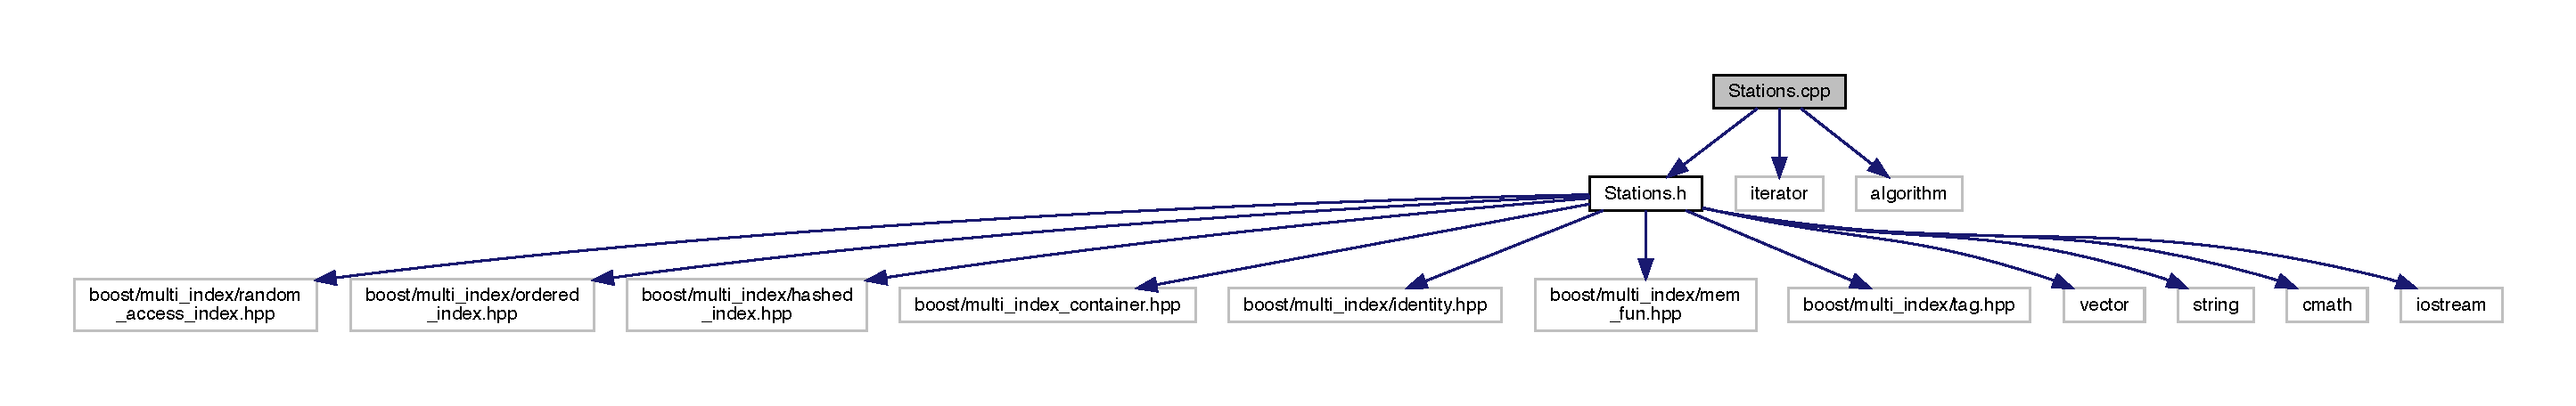
\includegraphics[width=350pt]{_stations_8cpp__incl}
\end{center}
\end{figure}
\subsection*{Functions}
\begin{DoxyCompactItemize}
\item 
ostream \& \mbox{\hyperlink{_stations_8cpp_ab01893ed80c5dcb0b0be727d12596bed}{operator$<$$<$}} (ostream \&os, \mbox{\hyperlink{class_station}{Station}} const \&obj)
\item 
ostream \& \mbox{\hyperlink{_stations_8cpp_a260395e1190ac92b92776902073ef760}{operator$<$$<$}} (ostream \&os, \mbox{\hyperlink{class_stations}{Stations}} const \&obj)
\end{DoxyCompactItemize}


\subsection{Function Documentation}
\mbox{\Hypertarget{_stations_8cpp_ab01893ed80c5dcb0b0be727d12596bed}\label{_stations_8cpp_ab01893ed80c5dcb0b0be727d12596bed}} 
\index{Stations.\+cpp@{Stations.\+cpp}!operator$<$$<$@{operator$<$$<$}}
\index{operator$<$$<$@{operator$<$$<$}!Stations.\+cpp@{Stations.\+cpp}}
\subsubsection{\texorpdfstring{operator$<$$<$()}{operator<<()}\hspace{0.1cm}{\footnotesize\ttfamily [1/2]}}
{\footnotesize\ttfamily ostream\& operator$<$$<$ (\begin{DoxyParamCaption}\item[{ostream \&}]{os,  }\item[{\mbox{\hyperlink{class_station}{Station}} const \&}]{obj }\end{DoxyParamCaption})}

\mbox{\Hypertarget{_stations_8cpp_a260395e1190ac92b92776902073ef760}\label{_stations_8cpp_a260395e1190ac92b92776902073ef760}} 
\index{Stations.\+cpp@{Stations.\+cpp}!operator$<$$<$@{operator$<$$<$}}
\index{operator$<$$<$@{operator$<$$<$}!Stations.\+cpp@{Stations.\+cpp}}
\subsubsection{\texorpdfstring{operator$<$$<$()}{operator<<()}\hspace{0.1cm}{\footnotesize\ttfamily [2/2]}}
{\footnotesize\ttfamily ostream\& operator$<$$<$ (\begin{DoxyParamCaption}\item[{ostream \&}]{os,  }\item[{\mbox{\hyperlink{class_stations}{Stations}} const \&}]{obj }\end{DoxyParamCaption})}


\hypertarget{_stations_8h}{}\section{Stations.\+h File Reference}
\label{_stations_8h}\index{Stations.\+h@{Stations.\+h}}
{\ttfamily \#include $<$vector$>$}\newline
{\ttfamily \#include $<$string$>$}\newline
{\ttfamily \#include $<$cmath$>$}\newline
{\ttfamily \#include $<$iostream$>$}\newline
{\ttfamily \#include $<$unordered\+\_\+map$>$}\newline
{\ttfamily \#include $<$utility$>$}\newline
Include dependency graph for Stations.\+h\+:
\nopagebreak
\begin{figure}[H]
\begin{center}
\leavevmode
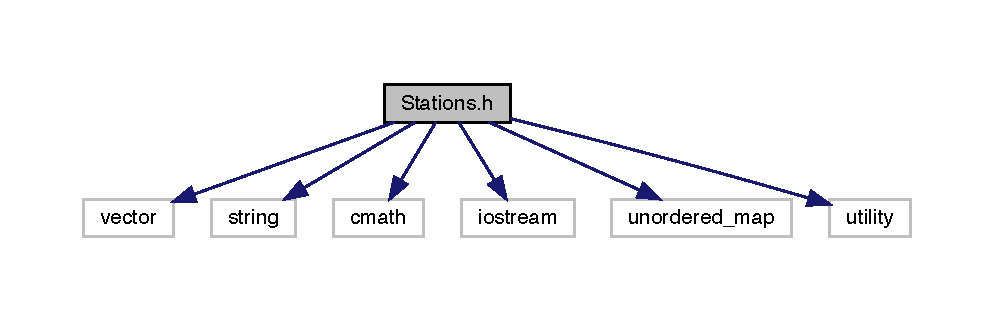
\includegraphics[width=350pt]{_stations_8h__incl}
\end{center}
\end{figure}
This graph shows which files directly or indirectly include this file\+:
\nopagebreak
\begin{figure}[H]
\begin{center}
\leavevmode
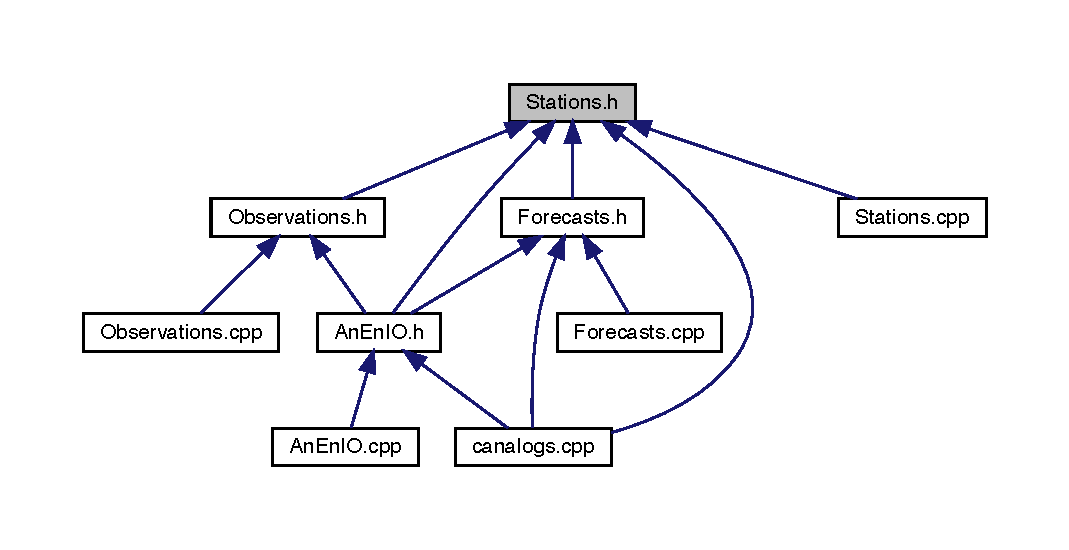
\includegraphics[width=350pt]{_stations_8h__dep__incl}
\end{center}
\end{figure}
\subsection*{Classes}
\begin{DoxyCompactItemize}
\item 
class \mbox{\hyperlink{class_station}{Station}}
\item 
class \mbox{\hyperlink{class_stations}{Stations}}
\end{DoxyCompactItemize}

\hypertarget{_times_8cpp}{}\section{Times.\+cpp File Reference}
\label{_times_8cpp}\index{Times.\+cpp@{Times.\+cpp}}
{\ttfamily \#include \char`\"{}Times.\+h\char`\"{}}\newline
{\ttfamily \#include $<$iterator$>$}\newline
Include dependency graph for Times.\+cpp\+:\nopagebreak
\begin{figure}[H]
\begin{center}
\leavevmode
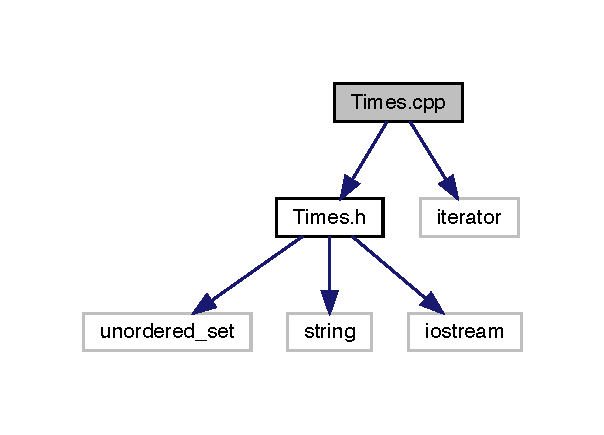
\includegraphics[width=350pt]{_times_8cpp__incl}
\end{center}
\end{figure}
\subsection*{Namespaces}
\begin{DoxyCompactItemize}
\item 
 \mbox{\hyperlink{namespaceanen_time}{anen\+Time}}
\end{DoxyCompactItemize}
\subsection*{Functions}
\begin{DoxyCompactItemize}
\item 
ostream \& \mbox{\hyperlink{namespaceanen_time_ab90a5dd8a6a0a1bd15220276fe8043b7}{anen\+Time\+::operator$<$$<$}} (ostream \&os, Times const \&obj)
\item 
ostream \& \mbox{\hyperlink{namespaceanen_time_a51b4045300f072275ce700d5b3362ca6}{anen\+Time\+::operator$<$$<$}} (ostream \&os, F\+L\+Ts const \&obj)
\end{DoxyCompactItemize}

\hypertarget{_times_8h}{}\section{Times.\+h File Reference}
\label{_times_8h}\index{Times.\+h@{Times.\+h}}
{\ttfamily \#include $<$string$>$}\newline
{\ttfamily \#include $<$iostream$>$}\newline
{\ttfamily \#include $<$boost/multi\+\_\+index/tag.\+hpp$>$}\newline
{\ttfamily \#include $<$boost/multi\+\_\+index/mem\+\_\+fun.\+hpp$>$}\newline
{\ttfamily \#include $<$boost/multi\+\_\+index\+\_\+container.\+hpp$>$}\newline
{\ttfamily \#include $<$boost/multi\+\_\+index/identity.\+hpp$>$}\newline
{\ttfamily \#include $<$boost/multi\+\_\+index/hashed\+\_\+index.\+hpp$>$}\newline
{\ttfamily \#include $<$boost/multi\+\_\+index/random\+\_\+access\+\_\+index.\+hpp$>$}\newline
Include dependency graph for Times.\+h\+:\nopagebreak
\begin{figure}[H]
\begin{center}
\leavevmode
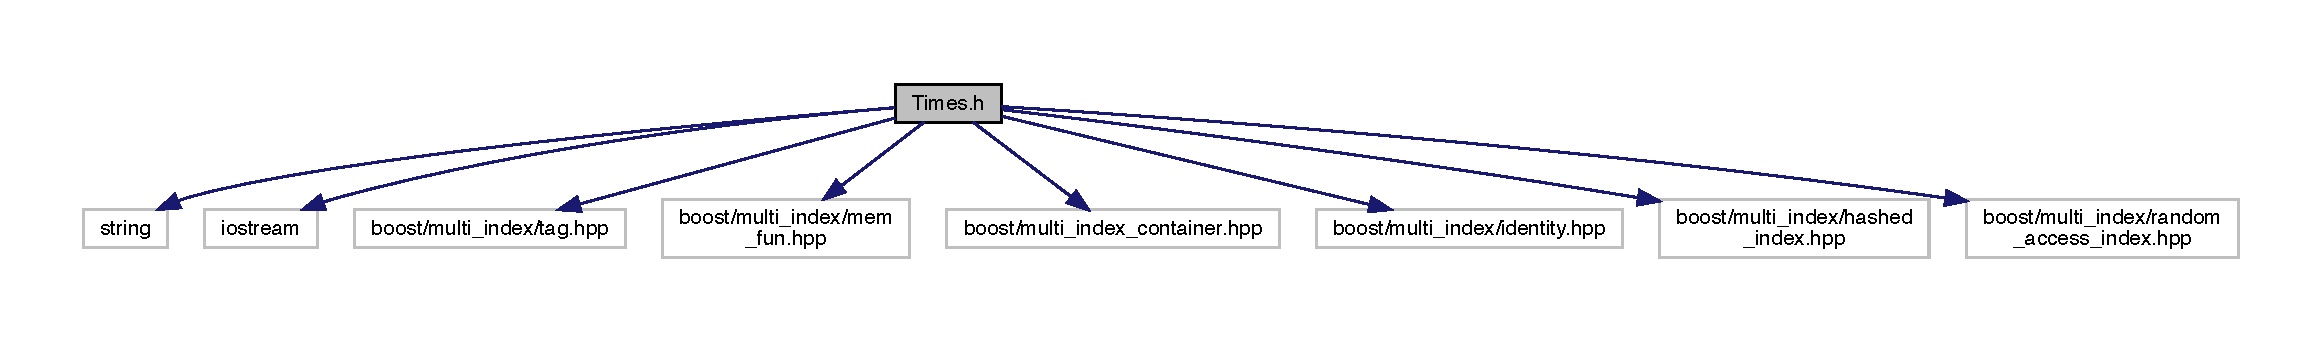
\includegraphics[width=350pt]{_times_8h__incl}
\end{center}
\end{figure}
This graph shows which files directly or indirectly include this file\+:
\nopagebreak
\begin{figure}[H]
\begin{center}
\leavevmode
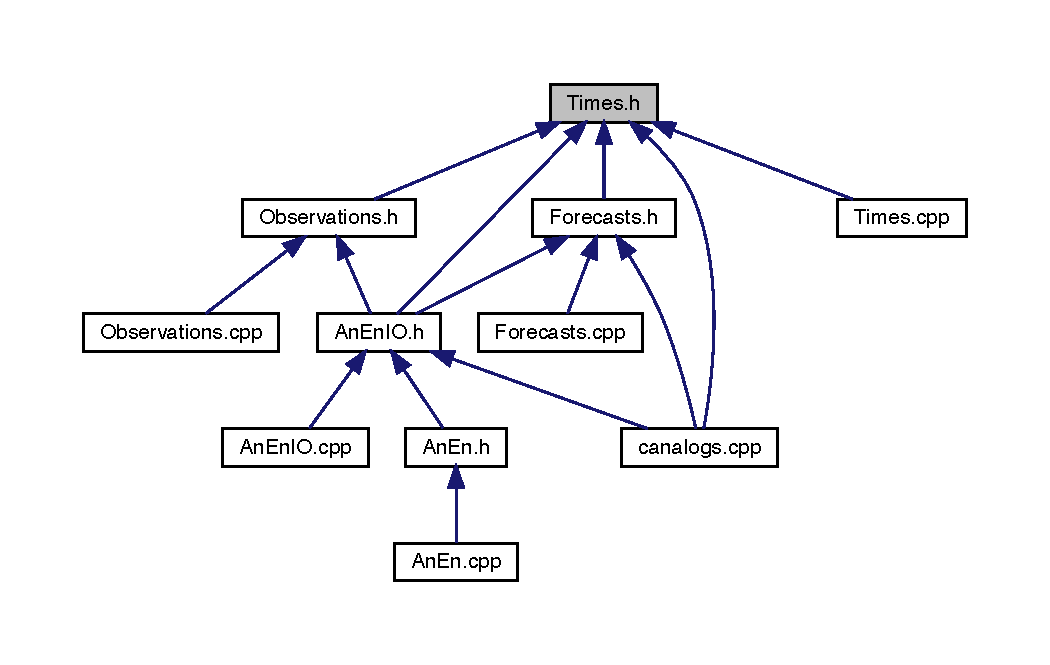
\includegraphics[width=350pt]{_times_8h__dep__incl}
\end{center}
\end{figure}
\subsection*{Classes}
\begin{DoxyCompactItemize}
\item 
struct \mbox{\hyperlink{structanen_time_1_1by__insert}{anen\+Time\+::by\+\_\+insert}}
\item 
struct \mbox{\hyperlink{structanen_time_1_1by__value}{anen\+Time\+::by\+\_\+value}}
\item 
class \mbox{\hyperlink{classanen_time_1_1_times}{anen\+Time\+::\+Times}}
\begin{DoxyCompactList}\small\item\em \mbox{\hyperlink{classanen_time_1_1_times}{Times}} class is used to store time information for predictions. By default this is the number of seconds from the origin January 1st, 1970. This can be customized by changing the default setting of origin and unit. \end{DoxyCompactList}\item 
class \mbox{\hyperlink{classanen_time_1_1_f_l_ts}{anen\+Time\+::\+F\+L\+Ts}}
\begin{DoxyCompactList}\small\item\em \mbox{\hyperlink{classanen_time_1_1_f_l_ts}{F\+L\+Ts}} class is used to store time information for prediction forecast lead times (\mbox{\hyperlink{classanen_time_1_1_f_l_ts}{F\+L\+Ts}}). If a temperature forecast on January 1st, 2028 contains predictions at 00h, 06h, 12h, 18h on that day, this forecast has 4 \mbox{\hyperlink{classanen_time_1_1_f_l_ts}{F\+L\+Ts}}, which are 0, 6, 12, 18. \end{DoxyCompactList}\end{DoxyCompactItemize}
\subsection*{Namespaces}
\begin{DoxyCompactItemize}
\item 
 \mbox{\hyperlink{namespaceanen_time}{anen\+Time}}
\end{DoxyCompactItemize}
\subsection*{Macros}
\begin{DoxyCompactItemize}
\item 
\#define \mbox{\hyperlink{_an_en_8cpp_a1d030df1b814e21fe6ccf3b46bcc12fa}{T\+I\+M\+E\+\_\+H}}
\end{DoxyCompactItemize}
\subsection*{Typedefs}
\begin{DoxyCompactItemize}
\item 
using \mbox{\hyperlink{namespaceanen_time_af2da8a18b50eb82edcc7b36e2a6b6441}{anen\+Time\+::multi\+Index\+Times}} = boost\+::multi\+\_\+index\+\_\+container$<$ double, boost\+::multi\+\_\+index\+::indexed\+\_\+by$<$ boost\+::multi\+\_\+index\+::random\+\_\+access$<$ boost\+::multi\+\_\+index\+::tag$<$ by\+\_\+insert $>$ $>$, boost\+::multi\+\_\+index\+::hashed\+\_\+unique$<$ boost\+::multi\+\_\+index\+::tag$<$ by\+\_\+value $>$, boost\+::multi\+\_\+index\+::identity$<$ std\+::size\+\_\+t $>$ $>$ $>$ $>$
\end{DoxyCompactItemize}


\subsection{Macro Definition Documentation}
\mbox{\Hypertarget{_an_en_8cpp_a1d030df1b814e21fe6ccf3b46bcc12fa}\label{_an_en_8cpp_a1d030df1b814e21fe6ccf3b46bcc12fa}} 
\index{Times.\+h@{Times.\+h}!T\+I\+M\+E\+\_\+H@{T\+I\+M\+E\+\_\+H}}
\index{T\+I\+M\+E\+\_\+H@{T\+I\+M\+E\+\_\+H}!Times.\+h@{Times.\+h}}
\subsubsection{\texorpdfstring{T\+I\+M\+E\+\_\+H}{TIME\_H}}
{\footnotesize\ttfamily \#define T\+I\+M\+E\+\_\+H}


%--- End generated contents ---

% Index
\backmatter
\newpage
\phantomsection
\clearemptydoublepage
\addcontentsline{toc}{chapter}{Index}
\printindex

\end{document}
